%%
% Copyright (c) 2017 - 2021, Pascal Wagler;
% Copyright (c) 2014 - 2021, John MacFarlane
%
% All rights reserved.
%
% Redistribution and use in source and binary forms, with or without
% modification, are permitted provided that the following conditions
% are met:
%
% - Redistributions of source code must retain the above copyright
% notice, this list of conditions and the following disclaimer.
%
% - Redistributions in binary form must reproduce the above copyright
% notice, this list of conditions and the following disclaimer in the
% documentation and/or other materials provided with the distribution.
%
% - Neither the name of John MacFarlane nor the names of other
% contributors may be used to endorse or promote products derived
% from this software without specific prior written permission.
%
% THIS SOFTWARE IS PROVIDED BY THE COPYRIGHT HOLDERS AND CONTRIBUTORS
% "AS IS" AND ANY EXPRESS OR IMPLIED WARRANTIES, INCLUDING, BUT NOT
% LIMITED TO, THE IMPLIED WARRANTIES OF MERCHANTABILITY AND FITNESS
% FOR A PARTICULAR PURPOSE ARE DISCLAIMED. IN NO EVENT SHALL THE
% COPYRIGHT OWNER OR CONTRIBUTORS BE LIABLE FOR ANY DIRECT, INDIRECT,
% INCIDENTAL, SPECIAL, EXEMPLARY, OR CONSEQUENTIAL DAMAGES (INCLUDING,
% BUT NOT LIMITED TO, PROCUREMENT OF SUBSTITUTE GOODS OR SERVICES;
% LOSS OF USE, DATA, OR PROFITS; OR BUSINESS INTERRUPTION) HOWEVER
% CAUSED AND ON ANY THEORY OF LIABILITY, WHETHER IN CONTRACT, STRICT
% LIABILITY, OR TORT (INCLUDING NEGLIGENCE OR OTHERWISE) ARISING IN
% ANY WAY OUT OF THE USE OF THIS SOFTWARE, EVEN IF ADVISED OF THE
% POSSIBILITY OF SUCH DAMAGE.
%%

%%
% This is the Eisvogel pandoc LaTeX template.
%
% For usage information and examples visit the official GitHub page:
% https://github.com/Wandmalfarbe/pandoc-latex-template
%%

% Options for packages loaded elsewhere
\PassOptionsToPackage{unicode}{hyperref}
\PassOptionsToPackage{hyphens}{url}
\PassOptionsToPackage{dvipsnames,svgnames,x11names,table}{xcolor}
%
\documentclass[
  a4paperpaper,
  ,captions=tableheading
]{scrbook}
\usepackage{amsmath,amssymb}
\usepackage{lmodern}
\usepackage{setspace}
\setstretch{1.2}
\usepackage{iftex}
\ifPDFTeX
  \usepackage[T1]{fontenc}
  \usepackage[utf8]{inputenc}
  \usepackage{textcomp} % provide euro and other symbols
\else % if luatex or xetex
  \usepackage{unicode-math}
  \defaultfontfeatures{Scale=MatchLowercase}
  \defaultfontfeatures[\rmfamily]{Ligatures=TeX,Scale=1}
\fi
% Use upquote if available, for straight quotes in verbatim environments
\IfFileExists{upquote.sty}{\usepackage{upquote}}{}
\IfFileExists{microtype.sty}{% use microtype if available
  \usepackage[]{microtype}
  \UseMicrotypeSet[protrusion]{basicmath} % disable protrusion for tt fonts
}{}
\makeatletter
\@ifundefined{KOMAClassName}{% if non-KOMA class
  \IfFileExists{parskip.sty}{%
    \usepackage{parskip}
  }{% else
    \setlength{\parindent}{0pt}
    \setlength{\parskip}{6pt plus 2pt minus 1pt}}
}{% if KOMA class
  \KOMAoptions{parskip=half}}
\makeatother
\usepackage{xcolor}
\definecolor{default-linkcolor}{HTML}{A50000}
\definecolor{default-filecolor}{HTML}{A50000}
\definecolor{default-citecolor}{HTML}{4077C0}
\definecolor{default-urlcolor}{HTML}{4077C0}
\IfFileExists{xurl.sty}{\usepackage{xurl}}{} % add URL line breaks if available
\IfFileExists{bookmark.sty}{\usepackage{bookmark}}{\usepackage{hyperref}}
\hypersetup{
  pdftitle={Music Memes},
  pdfauthor={Fabian C. Moss},
  colorlinks=true,
  linkcolor={blue},
  filecolor={default-filecolor},
  citecolor={default-citecolor},
  urlcolor={default-urlcolor},
  breaklinks=true,
  pdfcreator={LaTeX via pandoc with the Eisvogel template}}
\urlstyle{same} % disable monospaced font for URLs
\usepackage[margin=2.5cm,includehead=true,includefoot=true,centering,]{geometry}
\usepackage{color}
\usepackage{fancyvrb}
\newcommand{\VerbBar}{|}
\newcommand{\VERB}{\Verb[commandchars=\\\{\}]}
\DefineVerbatimEnvironment{Highlighting}{Verbatim}{commandchars=\\\{\}}
% Add ',fontsize=\small' for more characters per line
\usepackage{framed}
\definecolor{shadecolor}{RGB}{241,243,245}
\newenvironment{Shaded}{\begin{snugshade}}{\end{snugshade}}
\newcommand{\AlertTok}[1]{\textcolor[rgb]{0.68,0.00,0.00}{#1}}
\newcommand{\AnnotationTok}[1]{\textcolor[rgb]{0.37,0.37,0.37}{#1}}
\newcommand{\AttributeTok}[1]{\textcolor[rgb]{0.40,0.45,0.13}{#1}}
\newcommand{\BaseNTok}[1]{\textcolor[rgb]{0.68,0.00,0.00}{#1}}
\newcommand{\BuiltInTok}[1]{\textcolor[rgb]{0.00,0.23,0.31}{#1}}
\newcommand{\CharTok}[1]{\textcolor[rgb]{0.13,0.47,0.30}{#1}}
\newcommand{\CommentTok}[1]{\textcolor[rgb]{0.37,0.37,0.37}{#1}}
\newcommand{\CommentVarTok}[1]{\textcolor[rgb]{0.37,0.37,0.37}{\textit{#1}}}
\newcommand{\ConstantTok}[1]{\textcolor[rgb]{0.56,0.35,0.01}{#1}}
\newcommand{\ControlFlowTok}[1]{\textcolor[rgb]{0.00,0.23,0.31}{#1}}
\newcommand{\DataTypeTok}[1]{\textcolor[rgb]{0.68,0.00,0.00}{#1}}
\newcommand{\DecValTok}[1]{\textcolor[rgb]{0.68,0.00,0.00}{#1}}
\newcommand{\DocumentationTok}[1]{\textcolor[rgb]{0.37,0.37,0.37}{\textit{#1}}}
\newcommand{\ErrorTok}[1]{\textcolor[rgb]{0.68,0.00,0.00}{#1}}
\newcommand{\ExtensionTok}[1]{\textcolor[rgb]{0.00,0.23,0.31}{#1}}
\newcommand{\FloatTok}[1]{\textcolor[rgb]{0.68,0.00,0.00}{#1}}
\newcommand{\FunctionTok}[1]{\textcolor[rgb]{0.28,0.35,0.67}{#1}}
\newcommand{\ImportTok}[1]{\textcolor[rgb]{0.00,0.46,0.62}{#1}}
\newcommand{\InformationTok}[1]{\textcolor[rgb]{0.37,0.37,0.37}{#1}}
\newcommand{\KeywordTok}[1]{\textcolor[rgb]{0.00,0.23,0.31}{#1}}
\newcommand{\NormalTok}[1]{\textcolor[rgb]{0.00,0.23,0.31}{#1}}
\newcommand{\OperatorTok}[1]{\textcolor[rgb]{0.37,0.37,0.37}{#1}}
\newcommand{\OtherTok}[1]{\textcolor[rgb]{0.00,0.23,0.31}{#1}}
\newcommand{\PreprocessorTok}[1]{\textcolor[rgb]{0.68,0.00,0.00}{#1}}
\newcommand{\RegionMarkerTok}[1]{\textcolor[rgb]{0.00,0.23,0.31}{#1}}
\newcommand{\SpecialCharTok}[1]{\textcolor[rgb]{0.37,0.37,0.37}{#1}}
\newcommand{\SpecialStringTok}[1]{\textcolor[rgb]{0.13,0.47,0.30}{#1}}
\newcommand{\StringTok}[1]{\textcolor[rgb]{0.13,0.47,0.30}{#1}}
\newcommand{\VariableTok}[1]{\textcolor[rgb]{0.07,0.07,0.07}{#1}}
\newcommand{\VerbatimStringTok}[1]{\textcolor[rgb]{0.13,0.47,0.30}{#1}}
\newcommand{\WarningTok}[1]{\textcolor[rgb]{0.37,0.37,0.37}{\textit{#1}}}

% Workaround/bugfix from jannick0.
% See https://github.com/jgm/pandoc/issues/4302#issuecomment-360669013)
% or https://github.com/Wandmalfarbe/pandoc-latex-template/issues/2
%
% Redefine the verbatim environment 'Highlighting' to break long lines (with
% the help of fvextra). Redefinition is necessary because it is unlikely that
% pandoc includes fvextra in the default template.
\usepackage{fvextra}
\DefineVerbatimEnvironment{Highlighting}{Verbatim}{breaklines,fontsize=\small,commandchars=\\\{\}}

\usepackage{longtable,booktabs,array}
\usepackage{calc} % for calculating minipage widths
% Correct order of tables after \paragraph or \subparagraph
\usepackage{etoolbox}
\makeatletter
\patchcmd\longtable{\par}{\if@noskipsec\mbox{}\fi\par}{}{}
\makeatother
% Allow footnotes in longtable head/foot
\IfFileExists{footnotehyper.sty}{\usepackage{footnotehyper}}{\usepackage{footnote}}
\makesavenoteenv{longtable}
% add backlinks to footnote references, cf. https://tex.stackexchange.com/questions/302266/make-footnote-clickable-both-ways
\usepackage{footnotebackref}
\usepackage{graphicx}
\makeatletter
\def\maxwidth{\ifdim\Gin@nat@width>\linewidth\linewidth\else\Gin@nat@width\fi}
\def\maxheight{\ifdim\Gin@nat@height>\textheight\textheight\else\Gin@nat@height\fi}
\makeatother
% Scale images if necessary, so that they will not overflow the page
% margins by default, and it is still possible to overwrite the defaults
% using explicit options in \includegraphics[width, height, ...]{}
\setkeys{Gin}{width=\maxwidth,height=\maxheight,keepaspectratio}
% Set default figure placement to htbp
\makeatletter
\def\fps@figure{htbp}
\makeatother
\setlength{\emergencystretch}{3em} % prevent overfull lines
\providecommand{\tightlist}{%
  \setlength{\itemsep}{0pt}\setlength{\parskip}{0pt}}
\setcounter{secnumdepth}{5}
% Make \paragraph and \subparagraph free-standing
\ifx\paragraph\undefined\else
  \let\oldparagraph\paragraph
  \renewcommand{\paragraph}[1]{\oldparagraph{#1}\mbox{}}
\fi
\ifx\subparagraph\undefined\else
  \let\oldsubparagraph\subparagraph
  \renewcommand{\subparagraph}[1]{\oldsubparagraph{#1}\mbox{}}
\fi
\newlength{\cslhangindent}
\setlength{\cslhangindent}{1.5em}
\newlength{\csllabelwidth}
\setlength{\csllabelwidth}{3em}
\newlength{\cslentryspacingunit} % times entry-spacing
\setlength{\cslentryspacingunit}{\parskip}
\newenvironment{CSLReferences}[2] % #1 hanging-ident, #2 entry spacing
 {% don't indent paragraphs
  \setlength{\parindent}{0pt}
  % turn on hanging indent if param 1 is 1
  \ifodd #1
  \let\oldpar\par
  \def\par{\hangindent=\cslhangindent\oldpar}
  \fi
  % set entry spacing
  \setlength{\parskip}{#2\cslentryspacingunit}
 }%
 {}
\usepackage{calc}
\newcommand{\CSLBlock}[1]{#1\hfill\break}
\newcommand{\CSLLeftMargin}[1]{\parbox[t]{\csllabelwidth}{#1}}
\newcommand{\CSLRightInline}[1]{\parbox[t]{\linewidth - \csllabelwidth}{#1}\break}
\newcommand{\CSLIndent}[1]{\hspace{\cslhangindent}#1}
\makeatletter
\@ifpackageloaded{tcolorbox}{}{\usepackage[skins,breakable]{tcolorbox}}
\@ifpackageloaded{fontawesome5}{}{\usepackage{fontawesome5}}
\definecolor{quarto-callout-color}{HTML}{909090}
\definecolor{quarto-callout-note-color}{HTML}{0758E5}
\definecolor{quarto-callout-important-color}{HTML}{CC1914}
\definecolor{quarto-callout-warning-color}{HTML}{EB9113}
\definecolor{quarto-callout-tip-color}{HTML}{00A047}
\definecolor{quarto-callout-caution-color}{HTML}{FC5300}
\definecolor{quarto-callout-color-frame}{HTML}{acacac}
\definecolor{quarto-callout-note-color-frame}{HTML}{4582ec}
\definecolor{quarto-callout-important-color-frame}{HTML}{d9534f}
\definecolor{quarto-callout-warning-color-frame}{HTML}{f0ad4e}
\definecolor{quarto-callout-tip-color-frame}{HTML}{02b875}
\definecolor{quarto-callout-caution-color-frame}{HTML}{fd7e14}
\makeatother
\makeatletter
\makeatother
\makeatletter
\@ifpackageloaded{bookmark}{}{\usepackage{bookmark}}
\makeatother
\makeatletter
\@ifpackageloaded{caption}{}{\usepackage{caption}}
\AtBeginDocument{%
\ifdefined\contentsname
  \renewcommand*\contentsname{Table of contents}
\else
  \newcommand\contentsname{Table of contents}
\fi
\ifdefined\listfigurename
  \renewcommand*\listfigurename{List of Figures}
\else
  \newcommand\listfigurename{List of Figures}
\fi
\ifdefined\listtablename
  \renewcommand*\listtablename{List of Tables}
\else
  \newcommand\listtablename{List of Tables}
\fi
\ifdefined\figurename
  \renewcommand*\figurename{Figure}
\else
  \newcommand\figurename{Figure}
\fi
\ifdefined\tablename
  \renewcommand*\tablename{Table}
\else
  \newcommand\tablename{Table}
\fi
}
\@ifpackageloaded{float}{}{\usepackage{float}}
\floatstyle{ruled}
\@ifundefined{c@chapter}{\newfloat{codelisting}{h}{lop}}{\newfloat{codelisting}{h}{lop}[chapter]}
\floatname{codelisting}{Listing}
\newcommand*\listoflistings{\listof{codelisting}{List of Listings}}
\makeatother
\makeatletter
\@ifpackageloaded{caption}{}{\usepackage{caption}}
\@ifpackageloaded{subcaption}{}{\usepackage{subcaption}}
\makeatother
\makeatletter
\@ifpackageloaded{tcolorbox}{}{\usepackage[skins,breakable]{tcolorbox}}
\makeatother
\makeatletter
\@ifundefined{shadecolor}{\definecolor{shadecolor}{rgb}{.97, .97, .97}}
\makeatother
\makeatletter
\@ifundefined{codebgcolor}{\definecolor{codebgcolor}{HTML}{f5f5f5}}
\makeatother
\makeatletter
\makeatother
\ifLuaTeX
  \usepackage{selnolig}  % disable illegal ligatures
\fi

\title{Music Memes}
\usepackage{etoolbox}
\makeatletter
\providecommand{\subtitle}[1]{% add subtitle to \maketitle
  \apptocmd{\@title}{\par {\large #1 \par}}{}{}
}
\makeatother
\subtitle{Understanding music transmission processes through cultural
evolution modeling}
\author{Fabian C. Moss}
\date{2023-02-14}



%%
%% added
%%


%
% for the background color of the title page
%
\usepackage{pagecolor}
\usepackage{afterpage}
\usepackage{tikz}
\usepackage[margin=2.5cm,includehead=true,includefoot=true,centering]{geometry}

%
% break urls
%
\PassOptionsToPackage{hyphens}{url}

%
% When using babel or polyglossia with biblatex, loading csquotes is recommended
% to ensure that quoted texts are typeset according to the rules of your main language.
%
\usepackage{csquotes}

%
% captions
%
\definecolor{caption-color}{HTML}{777777}
\usepackage[font={stretch=1.2}, textfont={color=caption-color}, position=top, skip=4mm, labelfont=bf, singlelinecheck=false, justification=raggedright]{caption}
\setcapindent{0em}

%
% blockquote
%
\definecolor{blockquote-border}{RGB}{221,221,221}
\definecolor{blockquote-text}{RGB}{119,119,119}
\usepackage{mdframed}
\newmdenv[rightline=false,bottomline=false,topline=false,linewidth=3pt,linecolor=blockquote-border,skipabove=\parskip]{customblockquote}
\renewenvironment{quote}{\begin{customblockquote}\list{}{\rightmargin=0em\leftmargin=0em}%
\item\relax\color{blockquote-text}\ignorespaces}{\unskip\unskip\endlist\end{customblockquote}}

%
% Source Sans Pro as the de­fault font fam­ily
% Source Code Pro for monospace text
%
% 'default' option sets the default
% font family to Source Sans Pro, not \sfdefault.
%
\ifnum 0\ifxetex 1\fi\ifluatex 1\fi=0 % if pdftex
    \usepackage[default]{sourcesanspro}
  \usepackage{sourcecodepro}
  \else % if not pdftex
    \usepackage[default]{sourcesanspro}
  \usepackage{sourcecodepro}

  % XeLaTeX specific adjustments for straight quotes: https://tex.stackexchange.com/a/354887
  % This issue is already fixed (see https://github.com/silkeh/latex-sourcecodepro/pull/5) but the
  % fix is still unreleased.
  % TODO: Remove this workaround when the new version of sourcecodepro is released on CTAN.
  \ifxetex
    \makeatletter
    \defaultfontfeatures[\ttfamily]
      { Numbers   = \sourcecodepro@figurestyle,
        Scale     = \SourceCodePro@scale,
        Extension = .otf }
    \setmonofont
      [ UprightFont    = *-\sourcecodepro@regstyle,
        ItalicFont     = *-\sourcecodepro@regstyle It,
        BoldFont       = *-\sourcecodepro@boldstyle,
        BoldItalicFont = *-\sourcecodepro@boldstyle It ]
      {SourceCodePro}
    \makeatother
  \fi
  \fi

%
% heading color
%
\definecolor{heading-color}{RGB}{40,40,40}
\addtokomafont{section}{\color{heading-color}}
% When using the classes report, scrreprt, book,
% scrbook or memoir, uncomment the following line.
%\addtokomafont{chapter}{\color{heading-color}}

%
% variables for title, author and date
%
\usepackage{titling}
\title{Music Memes}
\author{Fabian C. Moss}
\date{2023-02-14}

%
% tables
%

\definecolor{table-row-color}{HTML}{F5F5F5}
\definecolor{table-rule-color}{HTML}{999999}

%\arrayrulecolor{black!40}
\arrayrulecolor{table-rule-color}     % color of \toprule, \midrule, \bottomrule
\setlength\heavyrulewidth{0.3ex}      % thickness of \toprule, \bottomrule
\renewcommand{\arraystretch}{1.3}     % spacing (padding)


%
% remove paragraph indention
%
\setlength{\parindent}{0pt}
\setlength{\parskip}{6pt plus 2pt minus 1pt}
\setlength{\emergencystretch}{3em}  % prevent overfull lines

%
%
% Listings
%
%


%
% header and footer
%
\usepackage[headsepline,footsepline]{scrlayer-scrpage}

\newpairofpagestyles{eisvogel-header-footer}{
  \clearpairofpagestyles
  \ihead*{Music Memes}
  \chead*{}
  \ohead*{2023-02-14}
  \ifoot*{Fabian C. Moss}
  \cfoot*{}
  \ofoot*{\thepage}
  \addtokomafont{pageheadfoot}{\upshape}
}
\pagestyle{eisvogel-header-footer}

\deftripstyle{ChapterStyle}{}{}{}{}{\pagemark}{}
\renewcommand*{\chapterpagestyle}{ChapterStyle}


%%
%% end added
%%

\begin{document}

%%
%% begin titlepage
%%
\begin{titlepage}
\newgeometry{top=2cm, right=4cm, bottom=3cm, left=4cm}
\tikz[remember picture,overlay] \node[inner sep=0pt] at (current page.center){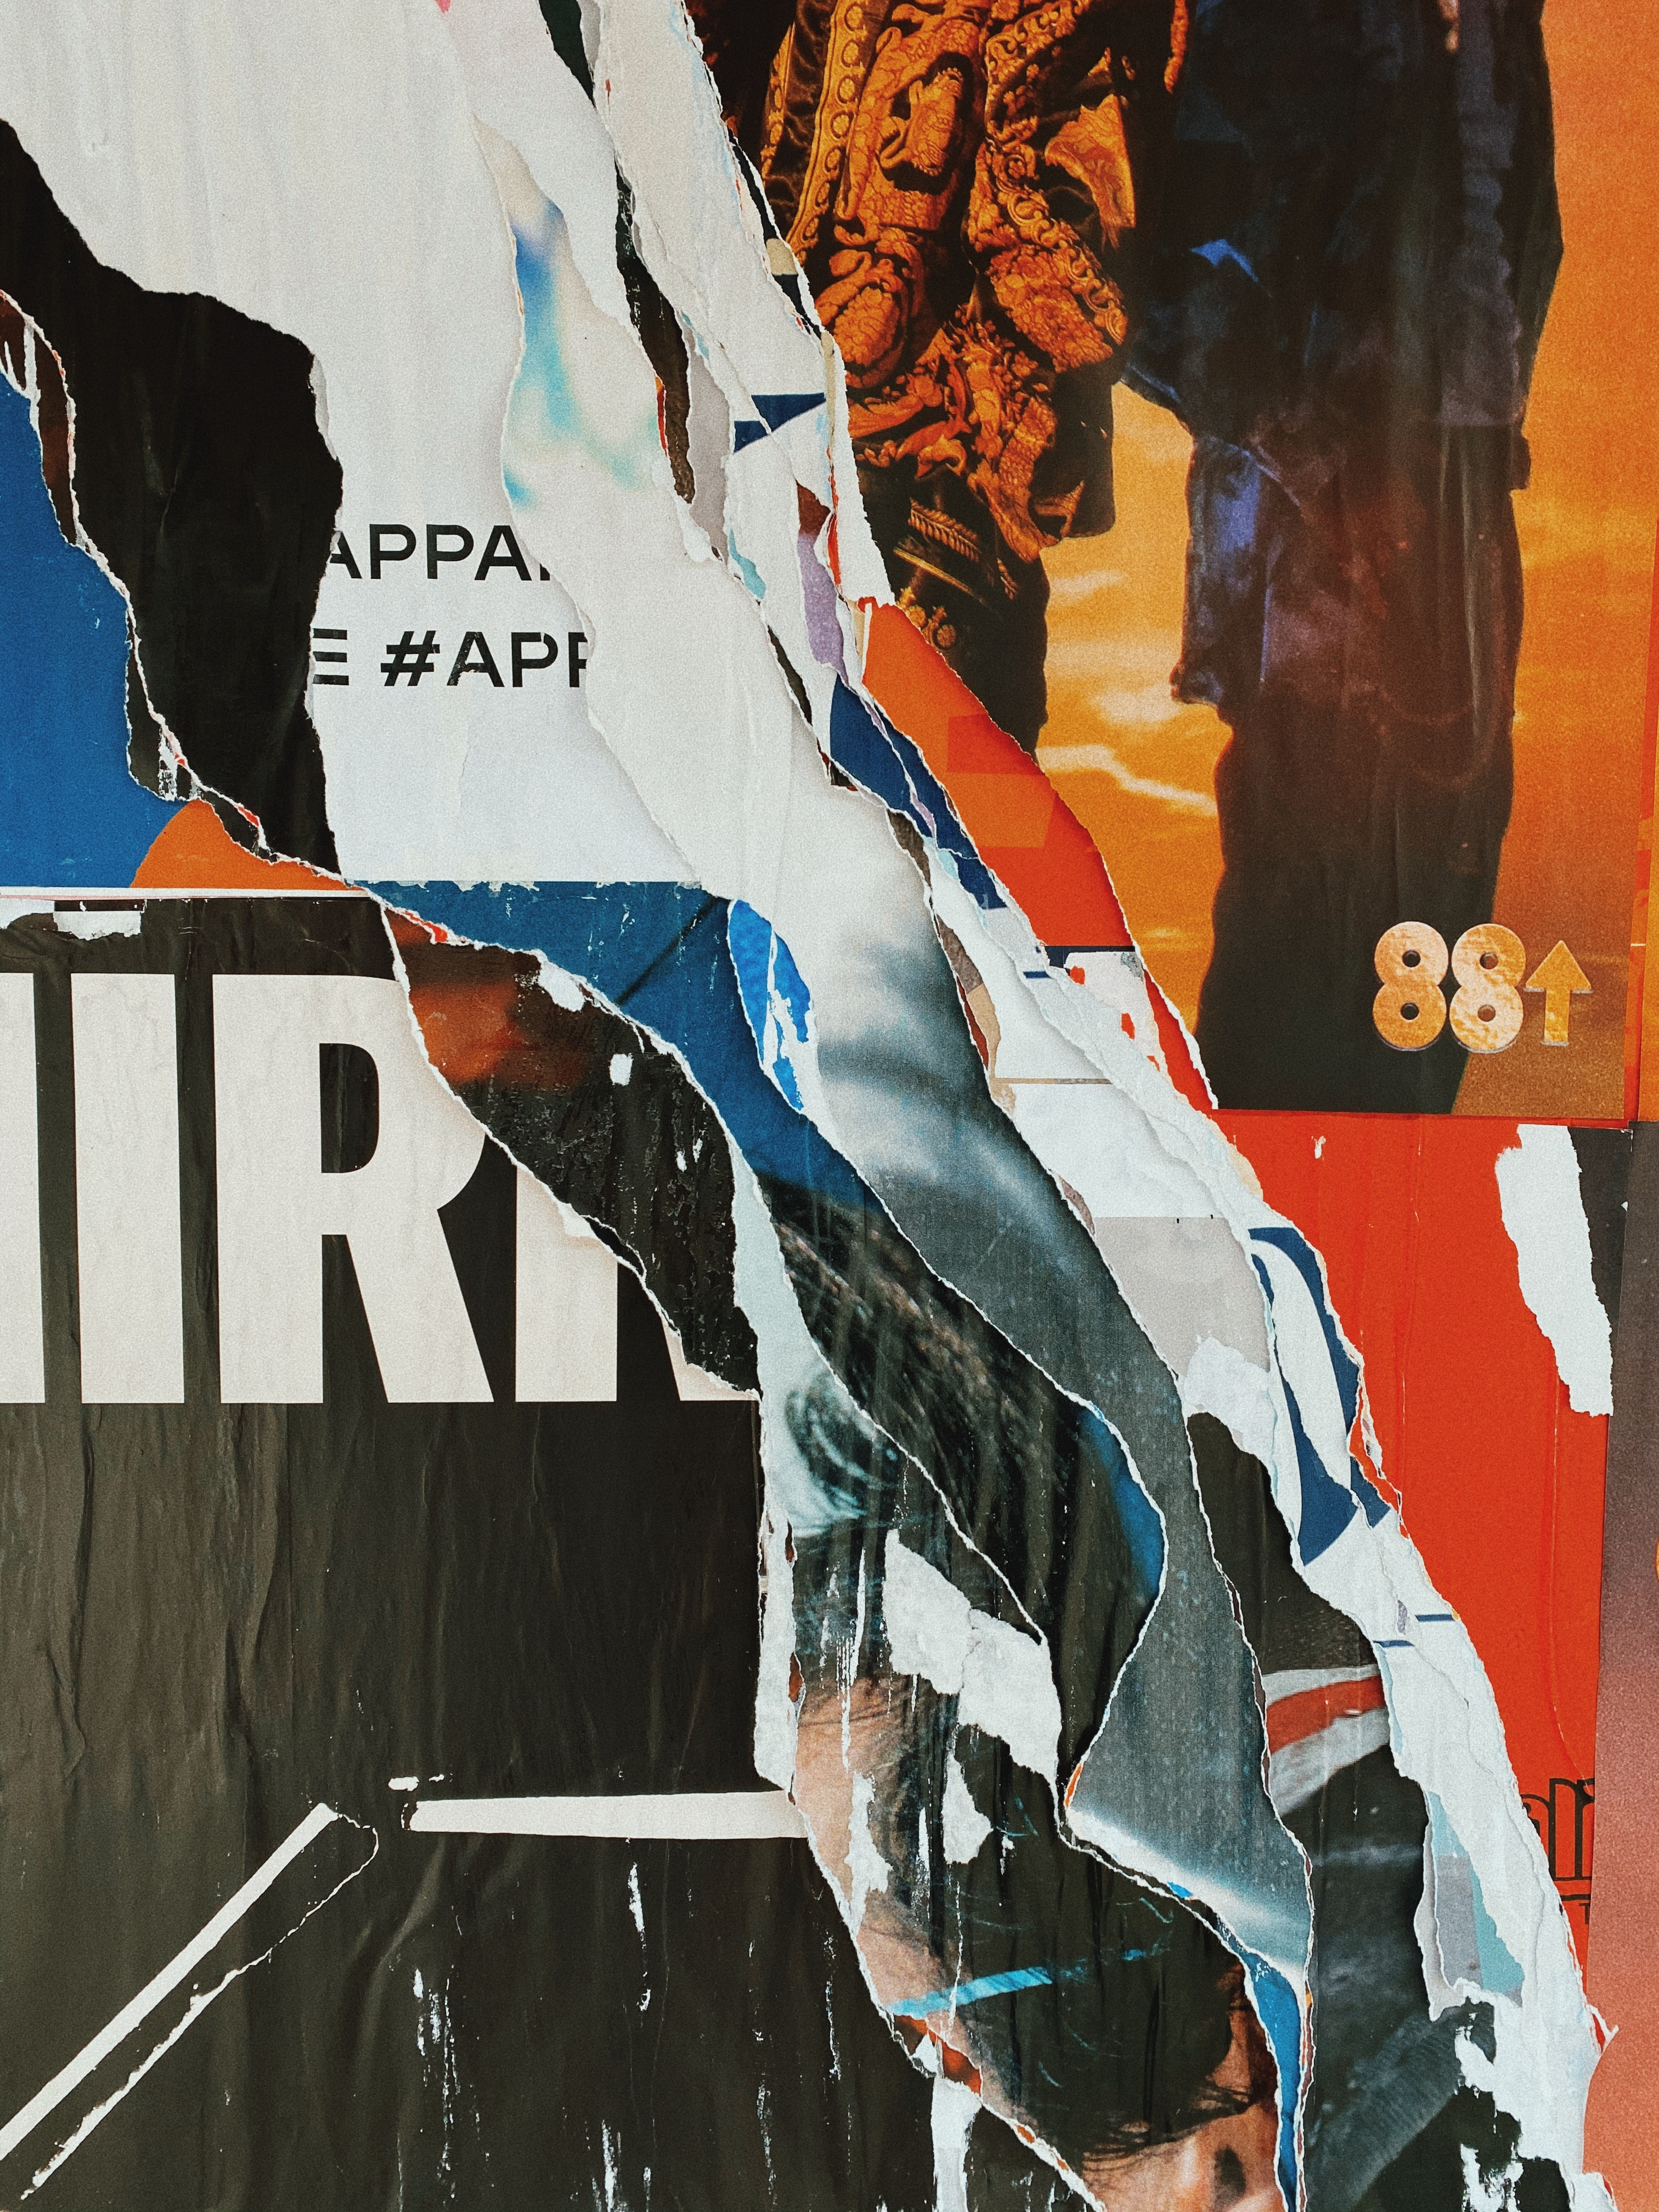
\includegraphics[width=\paperwidth,height=\paperheight]{texture.jpg}};
\newcommand{\colorRule}[3][black]{\textcolor[HTML]{#1}{\rule{#2}{#3}}}
\begin{flushleft}
\noindent
\\[-1em]
\color[HTML]{ffffff}
\makebox[0pt][l]{\colorRule[435488]{1.3\textwidth}{4pt}}
\par
\noindent

% The titlepage with a background image has other text spacing and text size
{
  \setstretch{2}
  \vfill
  \vskip -8em
  \noindent {\huge \textbf{\textsf{Music Memes}}}
    \vskip 1em
  {\Large \textsf{Understanding music transmission processes through
cultural evolution modeling}}
    \vskip 2em
  \noindent {\Large \textsf{Fabian C.
Moss} \vskip 0.6em \textsf{2023-02-14}}
  \vfill
}


\end{flushleft}
\end{titlepage}
\restoregeometry
\pagenumbering{arabic} 

%%
%% end titlepage
%%



\ifdefined\Shaded\renewenvironment{Shaded}{\begin{tcolorbox}[sharp corners, frame hidden, boxrule=0pt, breakable, enhanced, borderline west={3pt}{0pt}{shadecolor}, colback={codebgcolor}]}{\end{tcolorbox}}\fi

\renewcommand*\contentsname{Table of contents}
{
\hypersetup{linkcolor=}
\setcounter{tocdepth}{2}
\tableofcontents
}
\bookmarksetup{startatroot}

\hypertarget{welcome}{%
\chapter*{Welcome}\label{welcome}}
\addcontentsline{toc}{chapter}{Welcome}

\markboth{Welcome}{Welcome}

On these pages you will learn about cultural evolution and music. The
overall aim is to attain a basic understanding of formal models in
cultural evolution and learn about several recent approaches that apply
them to the domain of music.

We start with a minimal introduction to the
\href{https://www.python.org/}{Python} programming language that covers
the necessary basic skills in order to follow the remainder of the book.
Then, we summarize some general ideas about music and cultural
evolution.

Subsequently, we follow the excellent learning path for computational
models in cultural evolution provided by the book
\href{https://acerbialberto.com/IBM-cultevo/}{\emph{Individual-based
models of cultural evolution: A step-by-step guide using R}} (Acerbi et
al., 2022). These pages comprise a translation of this resource to
Python. Finally, we will review and discuss a number of recent
publications on music and cultural evolution in the advanced topics
section at the end.

\begin{tcolorbox}[enhanced jigsaw, arc=.35mm, left=2mm, colback=white, leftrule=.75mm, breakable, toprule=.15mm, opacityback=0, bottomrule=.15mm, rightrule=.15mm]

If you want to refer to this resource, please cite it as appropriately,
e.g.:

Moss, F. C. (2023). \emph{Music memes: Understanding music transmission
processes through cultural evolution modeling}.
\url{https://fabianmoss.github.io/musicmemes}

\end{tcolorbox}

\begin{tcolorbox}[enhanced jigsaw, arc=.35mm, colbacktitle=quarto-callout-important-color!10!white, colback=white, breakable, toprule=.15mm, title=\textcolor{quarto-callout-important-color}{\faExclamation}\hspace{0.5em}{Important}, left=2mm, bottomtitle=1mm, toptitle=1mm, leftrule=.75mm, opacitybacktitle=0.6, titlerule=0mm, opacityback=0, rightrule=.15mm, bottomrule=.15mm, coltitle=black, colframe=quarto-callout-important-color-frame]

The material on this page has been adapted and designed for my
musicology research seminar ``Music Memes: quantitative approaches and
theories of cultural transmission of music'' at
\href{https://uni-wuerzburg.de/}{Würzburg University}, Germany.

Note that the materials here are still under development. Please inform
me if you notice any errors or other issues.

\end{tcolorbox}

\hypertarget{acknowledgements}{%
\paragraph*{Acknowledgements}\label{acknowledgements}}
\addcontentsline{toc}{paragraph}{Acknowledgements}

I am grateful for encouragement from
\href{https://twitter.com/acerbialberto}{Alberto Acerbi} to continue
working on my Python translation of his book and many helpful comments.

\part{Prelude}

\hypertarget{introduction}{%
\chapter{Introduction}\label{introduction}}

\hypertarget{musical-memes}{%
\section{Musical Memes}\label{musical-memes}}

The term `meme' has been adopted by everyday language and is usually
associated with a certain image, superimposed with text, that is shared
on the internet and has a particular contextual meaning.

\begin{figure}

{\centering 
\includegraphics{img/music_meme.jpeg}

}

\caption{A musical meme. This image itself has been ended up here after
being passed along a chain of cultural transmission processes involving
several social media: a Google search for ``music meme'' led to an image
result pointing to
\href{https://www.classicfm.com/discover-music/humour/classical-music-memes-distract-from-practice/}{Classic
FM}, which, in turn, had taken this image from the instagram page of
user
\href{https://www.instagram.com/musicmemes.for.supertonicteens}{@musicmemes.for.supertonicteens}.}

\end{figure}

Originally, however, the definition of `meme' was much broader. Towards
the end of \emph{The Selfish Gene}, Richard Dawkins introduced the
concept as follows:

\begin{quote}
``We need {[}\ldots{]} a noun that conveys the idea of a unit of
cultural transmission, or a unit of \emph{imitation}. `Mimeme' comes
from a suitable Greek root,\footnote{\url{https://en.wikipedia.org/wiki/Mimesis}}
but I want a monosyllable word that sounds a bit like `gene'. I hope my
classicist friends will forgive me if I abbreviate mimeme to
\emph{meme}.'' Dawkins (1976, p. 192)
\end{quote}

Here, we adopt this original, more extensive concept of memes that, as
we will discover, comprises the more or less funny internet pictures as
a special case.

The field of cultural evolution emerged in the 1980's (e.g., Boyd \&
Richerson, 1985; Cavalli-Sforza \& Feldman, 1981), and has, in parallel
with the advancement of computational facilities, gained momentum.
Theories on cultural evolution share many facets with approaches on
memetics (Aunger, 2001; Blackmore, 2000; Dawkins, 1976; Howe \& Windram,
2011), a field that has also been applied to the case of music (Jan,
2016).

In recent years, several approaches have attempted to apply formal
models from cultural evolution to the domain of music.

In the present context, we first introduce some central ideas of
cultural evolution and review a few major publications for the domain of
music.

A few selected important contributions are:

\begin{itemize}
\tightlist
\item
  ``Cultural Transmission and Evolution: A Quantitative Approach''
  (Cavalli-Sforza \& Feldman, 1981)
\item
  ``Culture and the Evolutionary Process'' (Boyd \& Richerson, 1985)
\item
  ``The Memetics of Music'' (Jan, 2016)
\item
  ``Cultural Evolution and Music'' (Youngblood et al., forthcoming)
\item
  ``Cultural Evolution of Music'' (Savage, 2019)
\end{itemize}

\hypertarget{conditions-for-an-evolutionary-system}{%
\section{Conditions for an evolutionary
system}\label{conditions-for-an-evolutionary-system}}

\begin{itemize}
\tightlist
\item
  variation
\item
  selection
\item
  retention
\end{itemize}

See Blackmore (2000), Chapter 2 ``Universal Darwinism'' for an excellent
introduction.

These factors are, coincidentally, also central in the definition of
folk music put forward by the \emph{International Folk Music Council}:

\begin{quote}
``Folk music is the product of a musical tradition that has been evolved
through the process of oral transmission. The factors that shape the
tradition are: (i) continuity which links the present with the past;
(ii) variation which springs from the creative impulse of the individual
or the group; and (iii) selection by the community, which determines the
form or forms in which the music survives.'' (International Folk Music
Council, 1955, p. 23; see also Karpeles, 1955)
\end{quote}

It is interesting that many contempory definitions of music, for example
the aphoristic ``humanly structured sound'' one, do not refer explicitly
to modes or conditions of transmission.

\hypertarget{music-in-human-evolution}{%
\section{Music in human evolution}\label{music-in-human-evolution}}

This book is about the cultural evolution of music. It has to be
mentioned, however, that there is a large body of research on the
biological evolution of music. This research asks questions about with
which evolutionary advantages music endowed early humans, whether it is
something that we share with other animals or whether it makes us
unique. Some hold the view that music has no particularly relevant
evolutionary function at all (Pinker, 1997), while others see in it a
key to our success as a species (Cross, 2016).

Whatever the true role of music in the evolutionary history of humanity
may have been, it is most certainly a fascinating topic to reflect upon.
After all, human musical activity with dedicated instruments can be
traced back at least 20,000 years, although it seems more than likely
that human `musicking' dates back much further, since our own bodies and
voices already provided us with excellent musical instruments long
before the first instruments have been devised.

If you are interested in learning more about biological-evolutionary
aspects of music, I highly recommend to read, e.g. Wallin et al. (2001),
Morley (2013), Tomlinson (2018), and Honing (2018).

\hypertarget{history-and-cultural-evolution}{%
\section{History and cultural
evolution}\label{history-and-cultural-evolution}}

Documenting, describing, and interpreting changes in human culture is
what historians do. Accordingly, changes in music belong to the field of
music history, or historical musicology. However, most historians would
probably be hesitant to employ models, or worse: formal models, in order
to describe historical processes. The dictum ``history doesn't repeat
itself'' seems to raise a fundamental argument against such endeavors
that aim at explaining cultural or historical changes by means of
underlying latent `forces'. Modeling, in that view, seems to erroneously
assume that history is teleological -- directed towards a predetermined
goal.

On the other hand, it is undeniable that there are many aspects of
culture exhibit regularities and `progresses' that are hard to explain
if there are no guiding processes. Defining ``culture'' is, of course,
yet another difficult enterprise. Here, I follow more or less the
definition of Boyd \& Richerson (1985, p. 33): ``Culture is information
capable of affecting individuals' phenotypes which they acquire from
other conspecifics \emph{by teaching or imitation} {[}emphasis
mine{]}''.\footnote{I encourage you to read Chapter 3 of their seminal
  book in order to fully capture the meaning of this quote.} The part
important to us here is ``by teaching or imitation'', which is meant to
imply: \emph{not} by genetic inheritance. If humans can transmit
information by other means than genetic inheritance, and if these
transmission processes continue over many generations, then they are
worth studying. Rest assured, the assumption of a hidden goal towards
which all cultural processes are directed is not needed at all! I hope
that you will share this conviction after working through this material.

\hypertarget{schema-theory}{%
\section{Schema theory}\label{schema-theory}}

What are the units (the basic memes) in music? Schema theory proposes a
set of more or less fixed patterns, `schemata', that underly a large
body of music in the Baroque and Classical period (Gjerdingen, 2007).

Are schemata really memes? I would think not because they can not mutate
freely without losing their meaning. I rather think schemata `fall out'
of several combinatorial possibilities to traverse the diatonic scale,
and compositional mechanisms to elaborate and vary them. But this kind
of variation is very different than the one we talk about in this book.
Composed variation is very regular, not random, and relying both on the
melodic and metric structures in which it unfolds. Those, however, could
very well be understood as environments with very strong constraints
(being `out-of-scale' or `off-beat').

\hypertarget{basic-cultural-inheritance-mechanisms}{%
\section{Basic cultural inheritance
mechanisms}\label{basic-cultural-inheritance-mechanisms}}

Following this introduction, we introduce some minimal requirements to
use Python for this course (Chapter~\ref{sec-python_primer}).

Subsequently, we introduce with six central mechanisms for cultural
inheritance: unbiased transmission
(Chapter~\ref{sec-unbiased_transmission}), unbiased and biased mutation
(Chapter~\ref{sec-unbiased_biased_mutation}), directly biased
transmission (Chapter~\ref{sec-direct-biased-transmission}),
frequency-dependent indirectly biased transmission
(Chapter~\ref{sec-frequency-biased-transmission}), and
demonstrator-based indirectly biased transmission
(Chapter~\ref{sec-demonstrator-biased-transmission}). We follow up with
a chapter on vertical and horizontal transmission
(Chapter~\ref{sec-vertical-horizontal}), and finally introduce the
multiple traits model (Chapter~\ref{sec-multiple-traits}). The following
diagram gives an overview of these processes:

After having a firm grasp on how these processes can be modeled in
Python and how modeling results can be interpreted, we move to more
advanced topics, and more specifically into a number of recent exciting
results about cultural evolution and music. We conclude our journey
(Chapter~\ref{sec-conclusion}) with a more general discussion of the
implications of cultural evolution for how we think about music, on the
relevance of modeling in music research and the humanities more
generally, as well as on the great potential of this approach for future
research.

\hypertarget{progress}{%
\section{Progress?}\label{progress}}

Finally, at the end of this introduction, I want to circle back to an
important issue that has been central to many concerns surrounding the
application of evolutionary models to music, and to culture more
generally. I am speaking about notions of progress and teleology in the
sense that (cultural) evolution would be, in some sense, continuously
improving. And not only that, it would be guided towards a certain goal,
an optimal state of superiority. These concerns shouldn't be disregarded
too lightly, especially in view of the misunderstandings and harmful
consequences they have caused. On the other hand, we also need a
differentiated perspective on evolutionary theory, its assumptions, and
the extent to which one might apply it to cultural phenomena. I believe
that the generally critical attitude in the humanities can be, in fact,
a great catalyst to weed out inappropriate notions and interpretations.
However, what is needed in addition is also a certain openness to engage
in discussions with scientific approaches to culture and not an
unreflected (and thus uncritical) dismissal \emph{per se}. The general
attitude towards evolutionary thinking in biology and culture is nicely
summarized in a quote by Kwame Anthony Appiah:

\begin{quote}
Nowadays, it is clear that one of the most distinctive marks of our
species is that our inheritance is both biological \emph{and} cultural.
Each generation of human beings in a particular society can build on
what was learned by the ones before {[}\ldots{]}. What makes us the wise
species---\emph{sapiens}, remember is the Latin for ``wise''---is that
our genes make brans that allow us to pick up things from one another
that are \emph{not} in our genes. (Appiah, 2018, p. 122)
\end{quote}

This book wants to contribute to a fruitful discussion, provide entry
points for humanists to better understand computational evolutionary
models, and to show in which areas they have been and could be applied.
After all, all of academia, the humanities and the sciences alike, are
also subject of constant changes and adaptations to new environmental
conditions. Music research is no exception.

\hypertarget{style}{%
\chapter{Style}\label{style}}

\begin{itemize}
\tightlist
\item
  What is meant by `style'?
\item
  The role of learning: learning describes the acquisition of
  knowledge/information. Learning mechanisms have different names
  depending on the temporal scale: evolution, ontogenesis, development,
  learning
\end{itemize}

\hypertarget{a-model-of-style-in-music}{%
\section{A model of style in music}\label{a-model-of-style-in-music}}

A comprehensive model for theoretical treatment of style was proposed by
Meyer (1989). In a nutshell, he proposes a model where certain
constraints favor differnt kinds of patternings. He organises these
constraints hierarchically so that this model is suitable to describe a
variety of stylistic phenomena on different levels. This clear
separation is more conceptual and practical only for theoretical
discussions. In a real scenario, boundaries are often unclear or
ambigous.

\hypertarget{constraints}{%
\subsection{Constraints}\label{constraints}}

\begin{enumerate}
\def\labelenumi{\arabic{enumi}.}
\tightlist
\item
  Laws
\item
  Rules
\item
  Strategies
\end{enumerate}

\hypertarget{patterns}{%
\subsection{Patterns}\label{patterns}}

\begin{enumerate}
\def\labelenumi{\arabic{enumi}.}
\tightlist
\item
  Dialect
\item
  Idiom
\item
  Intraopus Style (here, we need a concept of ``work'', but the extended
  ``meme'' concept or ``memecomplex might also be useful'')
\end{enumerate}

\hypertarget{sec-python_primer}{%
\chapter{A Python primer}\label{sec-python_primer}}

\begin{tcolorbox}[enhanced jigsaw, arc=.35mm, colbacktitle=quarto-callout-note-color!10!white, colback=white, breakable, toprule=.15mm, title=\textcolor{quarto-callout-note-color}{\faInfo}\hspace{0.5em}{Note}, left=2mm, bottomtitle=1mm, toptitle=1mm, leftrule=.75mm, opacitybacktitle=0.6, titlerule=0mm, opacityback=0, rightrule=.15mm, bottomrule=.15mm, coltitle=black, colframe=quarto-callout-note-color-frame]

From now on, we will assume that you have a working Python installation
running on your computer. You can check this by typing the following
into a terminal/console/command line:

\begin{Shaded}
\begin{Highlighting}[]
\NormalTok{python {-}{-}version}
\end{Highlighting}
\end{Shaded}

If the version number starts with a 3, you're all set. If not, please
consider one of the many tutorials online on how to install Python.

\end{tcolorbox}

\hypertarget{variables-and-types}{%
\section{Variables and types}\label{variables-and-types}}

Variable assignment in Python is straight-forward. You choose a name for
the variable, and assign a value to it using the \texttt{=} operator,
for example:

\begin{Shaded}
\begin{Highlighting}[]
\NormalTok{x }\OperatorTok{=} \DecValTok{100}
\end{Highlighting}
\end{Shaded}

assigns the value \texttt{100} to the variable \texttt{x}. If we call
the variable now, we can see that it has the value we assigned to it:

\begin{Shaded}
\begin{Highlighting}[]
\NormalTok{x}
\end{Highlighting}
\end{Shaded}

\begin{verbatim}
100
\end{verbatim}

Of course, we can also assign things other than numbers, for example:

\begin{Shaded}
\begin{Highlighting}[]
\NormalTok{name }\OperatorTok{=} \StringTok{"Fabian"}
\end{Highlighting}
\end{Shaded}

What we assigned to the variable \texttt{name} is called a
\emph{string}, it has the value \texttt{"Fabian"}. Strings are sequences
of characters.

\begin{tcolorbox}[enhanced jigsaw, arc=.35mm, colbacktitle=quarto-callout-tip-color!10!white, colback=white, breakable, toprule=.15mm, title=\textcolor{quarto-callout-tip-color}{\faLightbulb}\hspace{0.5em}{Tip}, left=2mm, bottomtitle=1mm, toptitle=1mm, leftrule=.75mm, opacitybacktitle=0.6, titlerule=0mm, opacityback=0, rightrule=.15mm, bottomrule=.15mm, coltitle=black, colframe=quarto-callout-tip-color-frame]

Note that \texttt{"Fabian"} is enclosed by double-quotes. Why is this
the case? Why could we not just type \texttt{name\ =\ Fabian}?

\end{tcolorbox}

We can also assign a list of things to a variable:

\begin{Shaded}
\begin{Highlighting}[]
\NormalTok{mylist }\OperatorTok{=}\NormalTok{ [}\DecValTok{1}\NormalTok{, }\DecValTok{2}\NormalTok{, }\DecValTok{3}\NormalTok{, }\StringTok{"A"}\NormalTok{, }\StringTok{"B"}\NormalTok{, }\StringTok{"C"}\NormalTok{]}
\end{Highlighting}
\end{Shaded}

Lists are enclosed by square brackets. As you can see, Python allows you
to store any kind of data in lists (here: integer numbers and character
strings). However, it is good practice to include only items of the same
type in lists---you'll understand later why.

Another structured data type in python are dictionaries. Dictionaries
are collections of key-value pairs. For example, a dictionary
\texttt{addresses} could store the email addresses of certain people:

\begin{Shaded}
\begin{Highlighting}[]
\NormalTok{addresses }\OperatorTok{=}\NormalTok{ \{}
    \StringTok{"Andrew"}\NormalTok{ : }\StringTok{"andrew@example.com"}\NormalTok{,}
    \StringTok{"Zoe"}\NormalTok{ : }\StringTok{"zoe@example.com"}
\NormalTok{\}}
\end{Highlighting}
\end{Shaded}

Now, if we wanted to look up Zoe's email address, we could to so with:

\begin{Shaded}
\begin{Highlighting}[]
\NormalTok{addresses[}\StringTok{"Zoe"}\NormalTok{]}
\end{Highlighting}
\end{Shaded}

\begin{verbatim}
'zoe@example.com'
\end{verbatim}

\hypertarget{on-repeat}{%
\section{On repeat}\label{on-repeat}}

Coding something is only useful if you can't do the job as fast or as
efficient by yourself. Especially when it comes to repeating the same
little thing many, many times, knowing how to code comes in handy.

As a simple example, imagine you want to write down all numbers from 1
to 10, or from 1 to 100, or\ldots{} you get the idea. In Python, you
would do it as follows:

\begin{Shaded}
\begin{Highlighting}[]
\ControlFlowTok{for}\NormalTok{ i }\KeywordTok{in} \BuiltInTok{range}\NormalTok{(}\DecValTok{10}\NormalTok{):}
    \BuiltInTok{print}\NormalTok{(i)}
\end{Highlighting}
\end{Shaded}

\begin{verbatim}
0
1
2
3
4
5
6
7
8
9
\end{verbatim}

You see that this is not exactly what we wanted. We're seeing numbers
from 0 to 9, each one being printed on a new line. But what we wanted
was all numbers from 1 to 10. Before we fix the code to produce the
desired result, let's explain the bits and pieces of the code above.

What we just did was to use a so-called \emph{for-loop}, probably the
most common way to repeat things in Python. First we create an
\emph{iterator variable} \texttt{i} (we could have named any other
variable name as well), which takes its value from the list of numbers
specified by \texttt{range(10)}. If only one number \texttt{n} is
provided to \texttt{range(n)}, it will enumerate all numbers from 0 to
\texttt{n-1}. If instead two arguments are provided, the first one
determines the starting number, and the second one stands for the
terminating number minus one---confusing, right?

So, in order to enumerate all numbers from 1 to 10, we have to write
\texttt{range(1,11)}. Additionally, we can use the \texttt{end} keyword
of the \texttt{print} function that allows us to print all numbers in
one line, separated only by a single white space instead of each one on
a new line.

\begin{Shaded}
\begin{Highlighting}[]
\ControlFlowTok{for}\NormalTok{ i }\KeywordTok{in} \BuiltInTok{range}\NormalTok{(}\DecValTok{1}\NormalTok{,}\DecValTok{11}\NormalTok{):}
    \BuiltInTok{print}\NormalTok{(i, end}\OperatorTok{=}\StringTok{" "}\NormalTok{)}
\end{Highlighting}
\end{Shaded}

\begin{verbatim}
1 2 3 4 5 6 7 8 9 10 
\end{verbatim}

Voilà!

\hypertarget{just-in-case}{%
\section{Just in case}\label{just-in-case}}

Often we encounter a situation where we would execute some code
\textbf{only if} certain conditions are met. In python, this is done
with the \texttt{if} statement. For example, if we want to only print
the even numbers in the range from 1 to 10, we could adapt the code from
above as follows:

\begin{Shaded}
\begin{Highlighting}[]
\ControlFlowTok{for}\NormalTok{ i }\KeywordTok{in} \BuiltInTok{range}\NormalTok{(}\DecValTok{1}\NormalTok{,}\DecValTok{11}\NormalTok{):}
    \ControlFlowTok{if}\NormalTok{ i }\OperatorTok{\%} \DecValTok{2} \OperatorTok{==} \DecValTok{0}\NormalTok{:}
        \BuiltInTok{print}\NormalTok{(i, }\StringTok{"is even"}\NormalTok{)}
\end{Highlighting}
\end{Shaded}

\begin{verbatim}
2 is even
4 is even
6 is even
8 is even
10 is even
\end{verbatim}

You can read this as ``if the remainder of dividing i by 2 is zero, then
print `i is even'\,''.

Now, we could also want to print a similar statement in the case that
\texttt{i} is odd:

\begin{Shaded}
\begin{Highlighting}[]
\ControlFlowTok{for}\NormalTok{ i }\KeywordTok{in} \BuiltInTok{range}\NormalTok{(}\DecValTok{1}\NormalTok{,}\DecValTok{11}\NormalTok{):}
    \ControlFlowTok{if}\NormalTok{ i }\OperatorTok{\%} \DecValTok{2} \OperatorTok{==} \DecValTok{0}\NormalTok{:}
        \BuiltInTok{print}\NormalTok{(i, }\StringTok{"is even"}\NormalTok{)}
    \ControlFlowTok{else}\NormalTok{:}
        \BuiltInTok{print}\NormalTok{(i, }\StringTok{"is odd"}\NormalTok{)}
\end{Highlighting}
\end{Shaded}

\begin{verbatim}
1 is odd
2 is even
3 is odd
4 is even
5 is odd
6 is even
7 is odd
8 is even
9 is odd
10 is even
\end{verbatim}

And, finally, we could also have more than just one condition. An
if-statement allows for arbitrary many if-else clauses, with which we
can formulate several different conditions by writing \texttt{elif}
(shorthand for `or else if'):

\begin{Shaded}
\begin{Highlighting}[]
\ControlFlowTok{for}\NormalTok{ i }\KeywordTok{in} \BuiltInTok{range}\NormalTok{(}\DecValTok{1}\NormalTok{,}\DecValTok{11}\NormalTok{):}
    \ControlFlowTok{if}\NormalTok{ i }\OperatorTok{\%} \DecValTok{2} \OperatorTok{==} \DecValTok{0}\NormalTok{:}
        \BuiltInTok{print}\NormalTok{(i, }\StringTok{"is even"}\NormalTok{)}
    \ControlFlowTok{elif}\NormalTok{ i }\OperatorTok{\%} \DecValTok{3} \OperatorTok{==} \DecValTok{0}\NormalTok{:}
        \BuiltInTok{print}\NormalTok{(i, }\StringTok{"is divisible by 3"}\NormalTok{)}
    \ControlFlowTok{else}\NormalTok{:}
        \BuiltInTok{print}\NormalTok{(i, }\StringTok{"is odd"}\NormalTok{)}
\end{Highlighting}
\end{Shaded}

\begin{verbatim}
1 is odd
2 is even
3 is divisible by 3
4 is even
5 is odd
6 is even
7 is odd
8 is even
9 is divisible by 3
10 is even
\end{verbatim}

We now know when a number is even and when it is divisible by 3. But
what about numbers that are \emph{both} even \emph{and} divisible by 3?
We just add another condition to the \texttt{elif} statement and enclose
each condition in parentheses, so that Python knows how things group
together:

\begin{Shaded}
\begin{Highlighting}[]
\ControlFlowTok{for}\NormalTok{ i }\KeywordTok{in} \BuiltInTok{range}\NormalTok{(}\DecValTok{1}\NormalTok{,}\DecValTok{11}\NormalTok{):}
    \ControlFlowTok{if}\NormalTok{ i }\OperatorTok{\%} \DecValTok{2} \OperatorTok{==} \DecValTok{0}\NormalTok{:}
        \BuiltInTok{print}\NormalTok{(i, }\StringTok{"is even"}\NormalTok{)}
    \ControlFlowTok{elif}\NormalTok{ (i }\OperatorTok{\%} \DecValTok{2} \OperatorTok{==} \DecValTok{0}\NormalTok{) }\KeywordTok{and}\NormalTok{ (i }\OperatorTok{\%} \DecValTok{3} \OperatorTok{==} \DecValTok{0}\NormalTok{):}
        \BuiltInTok{print}\NormalTok{(i, }\StringTok{"is even and divisible by 3"}\NormalTok{)}
    \ControlFlowTok{else}\NormalTok{:}
        \BuiltInTok{print}\NormalTok{(i, }\StringTok{"is odd"}\NormalTok{)}
\end{Highlighting}
\end{Shaded}

\begin{verbatim}
1 is odd
2 is even
3 is odd
4 is even
5 is odd
6 is even
7 is odd
8 is even
9 is odd
10 is even
\end{verbatim}

Why did this not work? The number 6 is even \emph{and} divisible by 3!
The reason is that the three statements (\texttt{if}, \texttt{elif}, and
\texttt{else}) are being executed in the order that we wrote them down.
That means, that Python will first check for each number whether it is
even (and nothing more), and if it is, it will follow the instruction to
print it and go on to the next number. So, once we arrived at 6, the
programm will only check if the number is even. That is not the desired
result and we have to make a little change to it. We will switch the
conditions in the \texttt{if} and \texttt{elif} statements:

\begin{Shaded}
\begin{Highlighting}[]
\ControlFlowTok{for}\NormalTok{ i }\KeywordTok{in} \BuiltInTok{range}\NormalTok{(}\DecValTok{1}\NormalTok{,}\DecValTok{11}\NormalTok{):}
    \ControlFlowTok{if}\NormalTok{ (i }\OperatorTok{\%} \DecValTok{2} \OperatorTok{==} \DecValTok{0}\NormalTok{) }\KeywordTok{and}\NormalTok{ (i }\OperatorTok{\%} \DecValTok{3} \OperatorTok{==} \DecValTok{0}\NormalTok{):}
        \BuiltInTok{print}\NormalTok{(i, }\StringTok{"is even and divisible by 3"}\NormalTok{)}
    \ControlFlowTok{elif}\NormalTok{ i }\OperatorTok{\%} \DecValTok{2} \OperatorTok{==} \DecValTok{0}\NormalTok{:}
        \BuiltInTok{print}\NormalTok{(i, }\StringTok{"is even"}\NormalTok{)}
    \ControlFlowTok{else}\NormalTok{:}
        \BuiltInTok{print}\NormalTok{(i, }\StringTok{"is odd"}\NormalTok{)}
\end{Highlighting}
\end{Shaded}

\begin{verbatim}
1 is odd
2 is even
3 is odd
4 is even
5 is odd
6 is even and divisible by 3
7 is odd
8 is even
9 is odd
10 is even
\end{verbatim}

Now it works! Note that new never specified any conditions for the
\texttt{else} statement. This is because whatever follows it will be
executed in case none of the conditions in \texttt{if} or \texttt{elif}
are met.

\hypertarget{functions}{%
\section{Functions}\label{functions}}

With more and more experience in programming, it is likely that your
code will become more and more complex. That means that it will become
harder to keep track of what every piece of it is supposed to do. A good
strategy to deal with this is to aim for writing code that is
\emph{modular}: it can be broken down into smaller units (modules) that
are easier to understand. Moreover, it is sometimes necessary to reuse
the same code several times. It would, however, be inefficient to write
the same lines over and over again. With your code being modular you can
wrap the pieces that you need in several places into a \emph{function}.

Let's look at an example! Assume, your (fairly) complex code involves
calculating the sum of the squares of two numbers. In Python, we use the
\texttt{+} operator to calculate sums and the \texttt{**} operator to
raise a number to a certain power (\texttt{**2} for the square of a
number).

\begin{Shaded}
\begin{Highlighting}[]
\NormalTok{x }\OperatorTok{=} \DecValTok{3}
\NormalTok{y }\OperatorTok{=} \DecValTok{5}

\NormalTok{sum\_of\_squares }\OperatorTok{=}\NormalTok{ x}\OperatorTok{**}\DecValTok{2} \OperatorTok{+}\NormalTok{ y}\OperatorTok{**}\DecValTok{2}
\end{Highlighting}
\end{Shaded}

The variable \texttt{sum\_of\_squares} now contains the sum of squares
of \texttt{x=3} and \texttt{y=5}. We can inspect the result by calling
the variable:

\begin{Shaded}
\begin{Highlighting}[]
\NormalTok{sum\_of\_squares }
\end{Highlighting}
\end{Shaded}

\begin{verbatim}
34
\end{verbatim}

Now, imagine that you would have to do the same calculation several
times for different combinations of values for \texttt{x} and \texttt{y}
(and always keeping in mind that this stands in for much more complex
examples with several lines of code). We can code this in a function:

\begin{Shaded}
\begin{Highlighting}[]
\KeywordTok{def}\NormalTok{ func\_sum\_of\_squares(x, y):}
    \ControlFlowTok{return}\NormalTok{ x}\OperatorTok{**}\DecValTok{2} \OperatorTok{+}\NormalTok{ y}\OperatorTok{**}\DecValTok{2}
\end{Highlighting}
\end{Shaded}

Now, each time we want to calculate a sum of squares, we can do so by
simply invoking

\begin{Shaded}
\begin{Highlighting}[]
\NormalTok{func\_sum\_of\_squares(}\DecValTok{5}\NormalTok{,}\DecValTok{4}\NormalTok{)}
\end{Highlighting}
\end{Shaded}

\begin{verbatim}
41
\end{verbatim}

And, of course, we could chose a shorter name for the function as well,
although I would recommend to always use function names that make clear
what the function does:

\begin{Shaded}
\begin{Highlighting}[]
\NormalTok{f }\OperatorTok{=}\NormalTok{ func\_sum\_of\_squares}

\NormalTok{f(}\DecValTok{5}\NormalTok{,}\DecValTok{4}\NormalTok{)}
\end{Highlighting}
\end{Shaded}

\begin{verbatim}
41
\end{verbatim}

\hypertarget{libraries-youll-love}{%
\section{Libraries you'll love}\label{libraries-youll-love}}

Luckily, you don't have to programm all functions by yourself. There is
a huge community of Python programmers out there that works and
collaborates on several \emph{libraries}. A library is (more or less)
simply a collection of certain functions (and some more, but we don't
get into this here). This means, instead of writing a function yourself,
you can rely on functions that someone else has programmed.

\begin{tcolorbox}[enhanced jigsaw, arc=.35mm, colbacktitle=quarto-callout-caution-color!10!white, colback=white, breakable, toprule=.15mm, title=\textcolor{quarto-callout-caution-color}{\faFire}\hspace{0.5em}{Caution}, left=2mm, bottomtitle=1mm, toptitle=1mm, leftrule=.75mm, opacitybacktitle=0.6, titlerule=0mm, opacityback=0, rightrule=.15mm, bottomrule=.15mm, coltitle=black, colframe=quarto-callout-caution-color-frame]

Whether a Python library or function does actually do what it promises
is another story. Popular libraries with tens of thousands of users are
very trust-worthy because you can be almost sure that someone would have
noticed erroneous behavior. But it is certainly possible that
badly-maintained libraries contain errors. So be prudent when using the
code of others.

\end{tcolorbox}

\hypertarget{numpy}{%
\subsection{NumPy}\label{numpy}}

One of the most popular Python libaries is
\href{https://numpy.org/}{NumPy} for numerical computations. We will
rely a lot on the functions in this library, especially in order to draw
random samples---more on this later! To use the functions or variables
from this library, they have to be \emph{imported} so that you can use
them. There are several ways to do this. For example, you can import the
libary entirely:

\begin{Shaded}
\begin{Highlighting}[]
\ImportTok{import}\NormalTok{ numpy}
\end{Highlighting}
\end{Shaded}

Now, you can use the (approximated) value of \(\pi\) stored in this
library by typing

\begin{Shaded}
\begin{Highlighting}[]
\NormalTok{numpy.pi}
\end{Highlighting}
\end{Shaded}

\begin{verbatim}
3.141592653589793
\end{verbatim}

A different way is to just import everything from the library by writing

\begin{Shaded}
\begin{Highlighting}[]
\ImportTok{from}\NormalTok{ numpy }\ImportTok{import} \OperatorTok{*} 
\end{Highlighting}
\end{Shaded}

Here, the \texttt{*} stands for `everything'. Now, to use the value of
\(\pi\) we could simply type

\begin{Shaded}
\begin{Highlighting}[]
\NormalTok{pi}
\end{Highlighting}
\end{Shaded}

\begin{verbatim}
3.141592653589793
\end{verbatim}

This is, however discouraged for the following reason: imagine we had
another library, \texttt{numpy2} that also stores the value of \(\pi\),
but less precisely (e.g.~only as \texttt{3.14}). If we write

\begin{Shaded}
\begin{Highlighting}[]
\ImportTok{from}\NormalTok{ numpy }\ImportTok{import} \OperatorTok{*} 
\ImportTok{from}\NormalTok{ numpy2 }\ImportTok{import} \OperatorTok{*} 
\end{Highlighting}
\end{Shaded}

We would have imported the variables holding the value of \(\pi\) from
both libraries. But, because they have the same name \texttt{pi}. In
this case, \texttt{pi} would equal \texttt{3.14} because we imported
\texttt{numpy2} last. This is confusing and shouldn't be so! To avoid
this, it is better to keep references to imported libraries explicit. In
order not to have to type too much (we're all lazy, after all), we can
define an alias for the library.

\begin{Shaded}
\begin{Highlighting}[]
\ImportTok{import}\NormalTok{ numpy }\ImportTok{as}\NormalTok{ np}
\NormalTok{np.pi}
\end{Highlighting}
\end{Shaded}

\begin{verbatim}
3.141592653589793
\end{verbatim}

All functions of NumPy are now accessible with the prefix \texttt{np.}.

\hypertarget{pandas}{%
\subsection{Pandas}\label{pandas}}

\protect\hyperlink{todo}{TODO}

\hypertarget{matplotlib}{%
\subsection{Matplotlib}\label{matplotlib}}

\protect\hyperlink{todo}{TODO}

\hypertarget{summary}{%
\subsection{Summary}\label{summary}}

You can choose any alias when importing a library (it can even by longer
than the library name) but certain conventions have emerged that you're
encouraged to follow. Importing the most commonly used Python libraries
for data-science tasks (``The data science triad''), use the following:

\begin{Shaded}
\begin{Highlighting}[]
\ImportTok{import}\NormalTok{ numpy }\ImportTok{as}\NormalTok{ np }\CommentTok{\# for numerical computations}
\ImportTok{import}\NormalTok{ pandas }\ImportTok{as}\NormalTok{ pd }\CommentTok{\# for tabular data }
\ImportTok{import}\NormalTok{ matplotlib.pyplot }\ImportTok{as}\NormalTok{ plt }\CommentTok{\# for data visualization}
\end{Highlighting}
\end{Shaded}

We will use all three of them in the following chapters and you'll learn
to love them.

\begin{tcolorbox}[enhanced jigsaw, arc=.35mm, colbacktitle=quarto-callout-tip-color!10!white, colback=white, breakable, toprule=.15mm, title=\textcolor{quarto-callout-tip-color}{\faLightbulb}\hspace{0.5em}{Concepts covered}, left=2mm, bottomtitle=1mm, toptitle=1mm, leftrule=.75mm, opacitybacktitle=0.6, titlerule=0mm, opacityback=0, rightrule=.15mm, bottomrule=.15mm, coltitle=black, colframe=quarto-callout-tip-color-frame]

\begin{itemize}
\tightlist
\item
  variables
\item
  types (integers, strings, lists, dictionaries)
\item
  functions
\item
  libraries, importing and aliases
\end{itemize}

\end{tcolorbox}

\hypertarget{sec-randomness}{%
\chapter{Randomness and order}\label{sec-randomness}}

This course is about music and evolution, specifically about using
computational models to better understand the mechanisms underlying
certain evolutionary processes. In order to do so, we will often run
simulations to observe and interpret the resulting scenarios against the
backdrop of our modeling assumptions and our domain knowledge.

Simulations are useful because for many situations we are not able to
provide deterministic mathematical formulae to obtain outcomes from
inputs. Rather, we incorporate our knowledge about the world in a
computational model and use randomness to include the inherent
uncertainty about the exact outcomes of the simulations.

\begin{tcolorbox}[enhanced jigsaw, arc=.35mm, left=2mm, colback=white, leftrule=.75mm, breakable, toprule=.15mm, opacityback=0, bottomrule=.15mm, rightrule=.15mm]

Add section on probability.

\end{tcolorbox}

But randomness is a difficult concept to capture. For the purpose of
this book, we will simulate a speficic kind of randomness by sampling
from a certain set of items. Less technically, we can imagine a bag with
a certain number of balls in it, each having a certain color (multiple
balls can have the same color). A \emph{random uniform sample with
replacement} then corresponds to picking a ball from the bag without
looking in it and putting it back in the bag.

\hypertarget{random-draws-from-a-bag}{%
\section{Random draws from a bag}\label{random-draws-from-a-bag}}

Let's try this in Python. We will use the \texttt{random} modul of the
\emph{NumPy} library:

\begin{Shaded}
\begin{Highlighting}[]
\ImportTok{import}\NormalTok{ numpy }\ImportTok{as}\NormalTok{ np}
\NormalTok{rng }\OperatorTok{=}\NormalTok{ np.random.default\_rng() }\CommentTok{\# initialize a default random generator}

\NormalTok{bag }\OperatorTok{=} \BuiltInTok{range}\NormalTok{(}\DecValTok{4}\NormalTok{)}
\NormalTok{ball }\OperatorTok{=}\NormalTok{ rng.choice(bag)}

\BuiltInTok{print}\NormalTok{(ball)}
\end{Highlighting}
\end{Shaded}

\begin{verbatim}
1
\end{verbatim}

If this draw were really random, we would expect that each number is
equally likely. We can test this by repeating this procedure again and
again, tallying the result each time.

\begin{Shaded}
\begin{Highlighting}[]
\ImportTok{import}\NormalTok{ pandas }\ImportTok{as}\NormalTok{ pd}
\ImportTok{import}\NormalTok{ matplotlib.pyplot }\ImportTok{as}\NormalTok{ plt}

\NormalTok{samples }\OperatorTok{=}\NormalTok{ []}

\ControlFlowTok{for}\NormalTok{ i }\KeywordTok{in} \BuiltInTok{range}\NormalTok{(}\DecValTok{1000}\NormalTok{):}
\NormalTok{    ball }\OperatorTok{=}\NormalTok{ rng.choice(bag)}
\NormalTok{    samples.append(ball)}

\NormalTok{s }\OperatorTok{=}\NormalTok{ pd.Series(samples)}

\BuiltInTok{print}\NormalTok{(s.head(}\DecValTok{10}\NormalTok{))}
\BuiltInTok{print}\NormalTok{(s.value\_counts().sort\_index())}
\end{Highlighting}
\end{Shaded}

\begin{verbatim}
0    2
1    0
2    0
3    0
4    0
5    1
6    3
7    1
8    2
9    3
dtype: int64
\end{verbatim}

\begin{verbatim}
0    254
1    255
2    229
3    262
Name: count, dtype: int64
\end{verbatim}

The number are not exactly the same but pretty close. If we would
continue sampling from our bag, they would get more and more similar to
one another. It is easier to understand this by visualizing it.

\begin{Shaded}
\begin{Highlighting}[]
\NormalTok{s.value\_counts().sort\_index().plot(kind}\OperatorTok{=}\StringTok{"bar"}\NormalTok{)}
\NormalTok{plt.show()}
\end{Highlighting}
\end{Shaded}

\begin{figure}[H]

{\centering 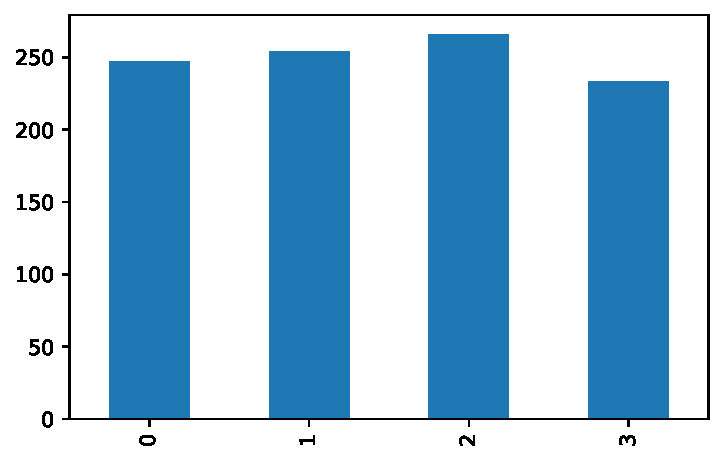
\includegraphics{randomness_files/figure-pdf/cell-4-output-1.pdf}

}

\end{figure}

Now, what if the numbers in the bag were not just numbered, but had
different colors? Let's assume we have another bag, \texttt{bag2}, with
4 balls, three brown, one blue:

\begin{Shaded}
\begin{Highlighting}[]
\NormalTok{bag2 }\OperatorTok{=}\NormalTok{ [ }\StringTok{"blue"}\NormalTok{, }\StringTok{"blue"}\NormalTok{, }\StringTok{"blue"}\NormalTok{, }\StringTok{"brown"}\NormalTok{ ]}

\NormalTok{samples2 }\OperatorTok{=}\NormalTok{ []}

\ControlFlowTok{for}\NormalTok{ i }\KeywordTok{in} \BuiltInTok{range}\NormalTok{(}\DecValTok{1000}\NormalTok{):}
\NormalTok{    ball }\OperatorTok{=}\NormalTok{ np.random.choice(bag2)}
\NormalTok{    samples2.append(ball)}

\NormalTok{s2 }\OperatorTok{=}\NormalTok{ pd.Series(samples2)}

\BuiltInTok{print}\NormalTok{(s2.head(}\DecValTok{10}\NormalTok{))}
\BuiltInTok{print}\NormalTok{(s2.value\_counts().sort\_index())}

\NormalTok{s2.value\_counts().sort\_index().plot(kind}\OperatorTok{=}\StringTok{"bar"}\NormalTok{)}
\NormalTok{plt.show()}
\end{Highlighting}
\end{Shaded}

\begin{verbatim}
0    brown
1     blue
2     blue
3     blue
4     blue
5     blue
6    brown
7     blue
8    brown
9    brown
dtype: object
blue     728
brown    272
Name: count, dtype: int64
\end{verbatim}

\begin{figure}[H]

{\centering 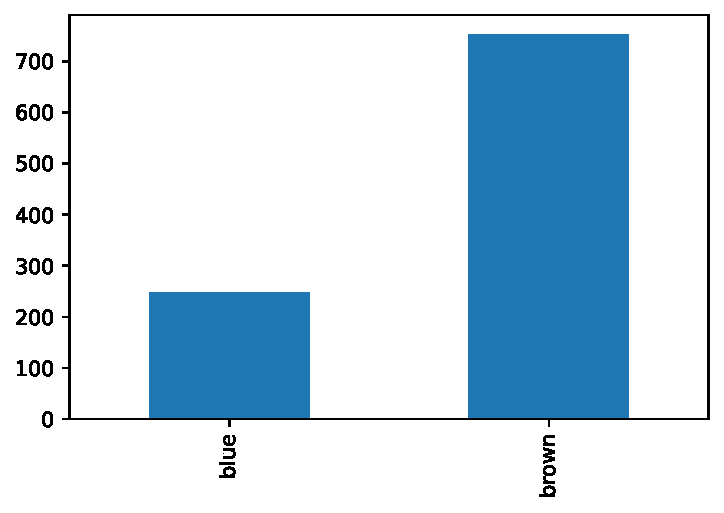
\includegraphics{randomness_files/figure-pdf/cell-5-output-2.pdf}

}

\end{figure}

This is remarkable: by randomly (uniformly) drawing from the second bag,
the frequencies of all samples approach the ratio of brown to blue balls
(3:1)!

\hypertarget{composing-random-melodies}{%
\section{Composing random melodies}\label{composing-random-melodies}}

Since this book is about music, let's see how we can use randomness to
create (a resemblance of) music. For instance, we can `compose' a random
melody by using only the white keys on a piano within some octave:

\begin{Shaded}
\begin{Highlighting}[]
\NormalTok{notes }\OperatorTok{=} \BuiltInTok{list}\NormalTok{(}\StringTok{"CDEFGAB"}\NormalTok{)}
\NormalTok{melody }\OperatorTok{=}\NormalTok{ rng.choice(notes, size}\OperatorTok{=}\DecValTok{10}\NormalTok{)}
\BuiltInTok{print}\NormalTok{(melody, end}\OperatorTok{=}\StringTok{" "}\NormalTok{)}
\end{Highlighting}
\end{Shaded}

\begin{verbatim}
['B' 'C' 'C' 'B' 'C' 'G' 'D' 'G' 'C' 'E'] 
\end{verbatim}

We composed a little melody by randomly drawing a note from the list of
notes. This is also called \emph{sampling}. Note that some notes repeat,
showing that we sample with replacement: after each draw, the note is
put back in the bag, so to speak. Of course, there are many things that
we would have to generate, too, to make this a real melody. For
instance, we do not know the duration of any of these notes, we don't
know the meter nor the key, we don't know the tempo or volume, and so
on. But our goal here is not to create a beautiful piece of music, but
rather to show how we can use randomness to generate something.

As you might remember from the previous chapter, we can also write a
function to do this, so that we can perform this operation (composition
of a random melody) more easily, while at the same time having more
control over it through its parameters. The following function does
exactly this, having only one parameter that controlls the length of the
melody (the number of notes to be sampled).

\begin{Shaded}
\begin{Highlighting}[]
\KeywordTok{def}\NormalTok{ melody(n):}
\NormalTok{    notes }\OperatorTok{=} \BuiltInTok{list}\NormalTok{(}\StringTok{"CDEFGAB"}\NormalTok{)}
    \ControlFlowTok{return}\NormalTok{ rng.choice(notes, size}\OperatorTok{=}\NormalTok{n)}
\end{Highlighting}
\end{Shaded}

We can now use this function to easily create random melodies of
different lengths:

\begin{Shaded}
\begin{Highlighting}[]
\BuiltInTok{print}\NormalTok{(melody(}\DecValTok{7}\NormalTok{))}
\end{Highlighting}
\end{Shaded}

\begin{verbatim}
['B' 'D' 'C' 'F' 'F' 'C' 'G']
\end{verbatim}

\begin{Shaded}
\begin{Highlighting}[]
\BuiltInTok{print}\NormalTok{(melody(}\DecValTok{12}\NormalTok{))}
\end{Highlighting}
\end{Shaded}

\begin{verbatim}
['G' 'E' 'G' 'G' 'F' 'A' 'D' 'A' 'B' 'F' 'E' 'D']
\end{verbatim}

\hypertarget{synthesizing-a-corpus}{%
\section{Synthesizing a corpus}\label{synthesizing-a-corpus}}

The functionalities introduced above allow us to synthesize an
artificial corpus of melodies, here simplified as lists of pitch classes
and containing varying numbers of notes.

\begin{Shaded}
\begin{Highlighting}[]
\NormalTok{N }\OperatorTok{=} \DecValTok{4} \CommentTok{\# number of pieces in the corpus}
\NormalTok{corpus }\OperatorTok{=}\NormalTok{ [ melody(}\DecValTok{12}\NormalTok{) }\ControlFlowTok{for}\NormalTok{ \_ }\KeywordTok{in} \BuiltInTok{range}\NormalTok{(N)]}
\end{Highlighting}
\end{Shaded}

The first three melodies of our corpus are:

\begin{Shaded}
\begin{Highlighting}[]
\ControlFlowTok{for}\NormalTok{ mel }\KeywordTok{in}\NormalTok{ corpus:}
    \BuiltInTok{print}\NormalTok{(mel)}
\end{Highlighting}
\end{Shaded}

\begin{verbatim}
['D' 'B' 'E' 'E' 'F' 'D' 'C' 'F' 'B' 'A' 'F' 'G']
['D' 'B' 'D' 'F' 'E' 'D' 'C' 'C' 'C' 'F' 'E' 'E']
['A' 'A' 'C' 'G' 'D' 'C' 'C' 'C' 'G' 'F' 'C' 'D']
['A' 'E' 'B' 'A' 'F' 'D' 'E' 'D' 'C' 'D' 'C' 'D']
\end{verbatim}

Of course, melodies are not always of the same length. We could vary the
lenght of the melodies by creating a hand-crafted list specifying the
number of notes for each melody in the corpus.

\begin{Shaded}
\begin{Highlighting}[]
\NormalTok{corpus }\OperatorTok{=}\NormalTok{ [ melody(n) }\ControlFlowTok{for}\NormalTok{ n }\KeywordTok{in}\NormalTok{ [}\DecValTok{10}\NormalTok{, }\DecValTok{5}\NormalTok{, }\DecValTok{7}\NormalTok{, }\DecValTok{13}\NormalTok{] ]}

\ControlFlowTok{for}\NormalTok{ mel }\KeywordTok{in}\NormalTok{ corpus:}
    \BuiltInTok{print}\NormalTok{(mel)}
\end{Highlighting}
\end{Shaded}

\begin{verbatim}
['G' 'E' 'G' 'E' 'F' 'C' 'G' 'D' 'C' 'E']
['D' 'B' 'B' 'B' 'A']
['D' 'C' 'G' 'C' 'G' 'D' 'B']
['F' 'B' 'D' 'A' 'D' 'G' 'D' 'G' 'B' 'F' 'E' 'F' 'A']
\end{verbatim}

However, specifying the lenghts of the melodies for a large corpus would
be a very time-consuming task. In order to model the variability in
length of melodies in a musical corpus, we will \emph{randomly sample}
them from a specified probability distribution. A good candidate for
such a distribution is the
\href{https://en.wikipedia.org/wiki/Poisson_distribution}{Poisson
distribution}, that we can access from our random number generator
\texttt{rng}.

\begin{Shaded}
\begin{Highlighting}[]
\NormalTok{lam }\OperatorTok{=} \DecValTok{25} \CommentTok{\# average number of notes in melody}
\NormalTok{N }\OperatorTok{=} \DecValTok{1000} \CommentTok{\# number of pieces in the corpus }

\NormalTok{corpus }\OperatorTok{=}\NormalTok{ [ melody(rng.poisson(lam}\OperatorTok{=}\NormalTok{lam)) }\ControlFlowTok{for}\NormalTok{ \_ }\KeywordTok{in} \BuiltInTok{range}\NormalTok{(N) ]}

\NormalTok{lengths }\OperatorTok{=}\NormalTok{ pd.Series([ }\BuiltInTok{len}\NormalTok{(m) }\ControlFlowTok{for}\NormalTok{ m }\KeywordTok{in}\NormalTok{ corpus ]).value\_counts()}

\NormalTok{idx }\OperatorTok{=} \BuiltInTok{range}\NormalTok{(}\DecValTok{0}\NormalTok{, }\BuiltInTok{max}\NormalTok{(lengths))}
\NormalTok{lengths }\OperatorTok{=}\NormalTok{ lengths.sort\_index().reindex(idx).fillna(}\DecValTok{0}\NormalTok{)}
\NormalTok{plt.bar(idx, lengths)}
\NormalTok{plt.axvline(lam, c}\OperatorTok{=}\StringTok{"red"}\NormalTok{)}
\NormalTok{plt.show()}
\end{Highlighting}
\end{Shaded}

\begin{figure}[H]

{\centering 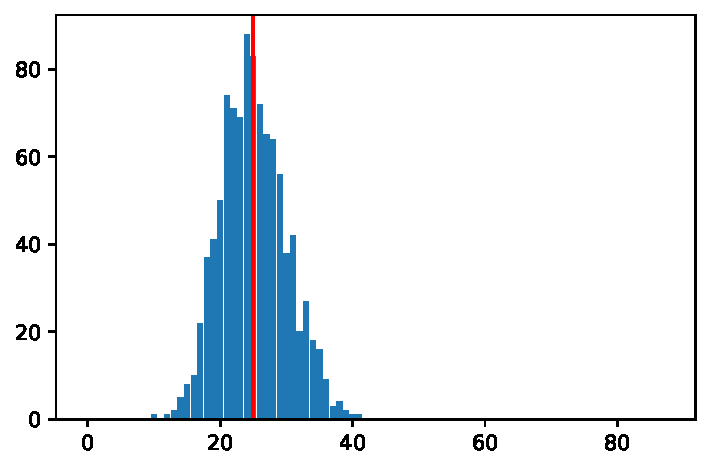
\includegraphics{randomness_files/figure-pdf/fig-piece-lengths-output-1.pdf}

}

\caption{\label{fig-piece-lengths}Distribution of melody lengths in the
corpus.''}

\end{figure}

Now the variable \texttt{corpus} contains lists of pitch classes
(\emph{aka} melodies) of different lengths, most of them around the
preset average value \texttt{lam},\footnote{Short for the Greek letter
  \(\lambda\) (``lambda'').} also indicated by the vertical red line. It
is moreover evident that the corpus contains rather few very short or
long melodies.

We can, of course, not only observe the distribution of melody lengths,
but also look at the overall distribution of note occurrence in the
corpus:

\begin{Shaded}
\begin{Highlighting}[]
\NormalTok{counts }\OperatorTok{=}\NormalTok{ []}

\ControlFlowTok{for}\NormalTok{ m }\KeywordTok{in}\NormalTok{ corpus:}
\NormalTok{    c }\OperatorTok{=}\NormalTok{ pd.Series(m)}
\NormalTok{    counts.append(c)}

\NormalTok{pd.concat(counts).value\_counts().plot(kind}\OperatorTok{=}\StringTok{"bar"}\NormalTok{)}
\NormalTok{plt.show()}
\end{Highlighting}
\end{Shaded}

\begin{figure}[H]

{\centering 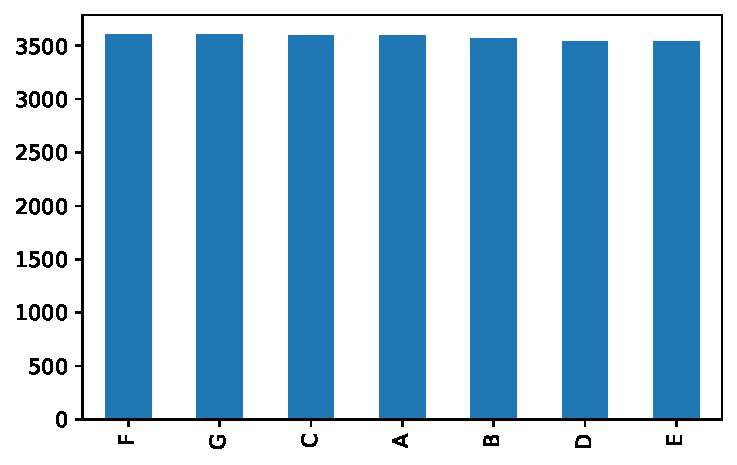
\includegraphics{randomness_files/figure-pdf/fig-note-freqs-output-1.pdf}

}

\caption{\label{fig-note-freqs}Overall note frequencies in the
artificial corpus.}

\end{figure}

At this point, we should stop and celebrate. We have just written our
first \emph{probabilistic model} to generate melodies. Admittedly, it is
not a very good model for actual melodies, for example because notes are
drawn \emph{uniformly at random} from the set of diatonic pitch classes
using the \texttt{.choice()} method, which leads to the somewhat
unrealistic picture in Figure~\ref{fig-note-freqs}. One would expect
that in real melodies some notes occur more often than others and that
the occurrence of a note does, for instance, also depend on the notes
that come before and after it. But, in principle, these other
constraints could be added to our model to make it more realistic. The
point here was mainly to illustrate how artificial corpora can be
generated probabilistically. This will prove useful later on because it
allows us to compare real-world corpora of music against synthetic ones
generated by our models.

\begin{tcolorbox}[enhanced jigsaw, arc=.35mm, colbacktitle=quarto-callout-tip-color!10!white, colback=white, breakable, toprule=.15mm, title=\textcolor{quarto-callout-tip-color}{\faLightbulb}\hspace{0.5em}{Exercise}, left=2mm, bottomtitle=1mm, toptitle=1mm, leftrule=.75mm, opacitybacktitle=0.6, titlerule=0mm, opacityback=0, rightrule=.15mm, bottomrule=.15mm, coltitle=black, colframe=quarto-callout-tip-color-frame]

Expand our melody model so that it also includes octave information for
each pitch class in order to make it a bit more musical.

\end{tcolorbox}

\hypertarget{pattern-search}{%
\section{Pattern search}\label{pattern-search}}

\hypertarget{incipits}{%
\subsection{Incipits}\label{incipits}}

Now that we have a corpus that we understand very well because we
specified how it has been created, we can apply some simple analytical
questions in order to warm up for later. For instance, we could want to
have a function that allows us to search for \emph{incipits}. Incipits
are the beginnings of musical melodies that already to characterize
themes and motives because incipits are often characteristic. For
example, we would want to look for all melodies that begin with ``C'',
``D'', ``E'' and, for simplicity, we might want to pass a string like
``CDE'' to the function to facilitate the input.

\begin{Shaded}
\begin{Highlighting}[]
\ImportTok{import}\NormalTok{ re }

\KeywordTok{def}\NormalTok{ find\_incipit(incip}\OperatorTok{=}\StringTok{""}\NormalTok{, mel}\OperatorTok{=}\VariableTok{None}\NormalTok{):}
\NormalTok{    melody }\OperatorTok{=} \StringTok{""}\NormalTok{.join(mel)}
    \ControlFlowTok{if}\NormalTok{ re.search(}\StringTok{"\^{}"} \OperatorTok{+}\NormalTok{ incip, melody):}
        \ControlFlowTok{return} \VariableTok{True}
    \ControlFlowTok{else}\NormalTok{:}
        \ControlFlowTok{return} \VariableTok{False}

\ControlFlowTok{for}\NormalTok{ m }\KeywordTok{in}\NormalTok{ corpus[:}\DecValTok{10}\NormalTok{]:}
    \ControlFlowTok{if}\NormalTok{ find\_incipit(incip}\OperatorTok{=}\StringTok{"CDE"}\NormalTok{, mel}\OperatorTok{=}\NormalTok{m):}
        \BuiltInTok{print}\NormalTok{(}\StringTok{""}\NormalTok{.join(m))}
\end{Highlighting}
\end{Shaded}

\hypertarget{finals}{%
\subsection{Finals}\label{finals}}

We can apply a similar logic to find finals, the last notes of a melody.
Instead of only allowing to search for a single note as a final, we will
allow more generally to allow for a pattern that concludes a melody:

\begin{Shaded}
\begin{Highlighting}[]
\KeywordTok{def}\NormalTok{ find\_finals(end}\OperatorTok{=}\StringTok{""}\NormalTok{, mel}\OperatorTok{=}\VariableTok{None}\NormalTok{):}
\NormalTok{    melody }\OperatorTok{=} \StringTok{""}\NormalTok{.join(mel)}
    \ControlFlowTok{if}\NormalTok{ re.search(end }\OperatorTok{+} \StringTok{"$"}\NormalTok{, melody):}
        \ControlFlowTok{return} \VariableTok{True} 

\ControlFlowTok{for}\NormalTok{ m }\KeywordTok{in}\NormalTok{ corpus[:}\DecValTok{100}\NormalTok{]:}
    \ControlFlowTok{if}\NormalTok{ find\_finals(end}\OperatorTok{=}\StringTok{"GC"}\NormalTok{, mel}\OperatorTok{=}\NormalTok{m):}
        \BuiltInTok{print}\NormalTok{(m)}
\end{Highlighting}
\end{Shaded}

\begin{verbatim}
['D' 'E' 'C' 'A' 'D' 'G' 'A' 'C' 'B' 'A' 'D' 'B' 'E' 'G' 'F' 'E' 'D' 'A'
 'B' 'C' 'C' 'F' 'C' 'D' 'E' 'D' 'F' 'G' 'C']
['F' 'F' 'B' 'E' 'E' 'C' 'G' 'B' 'C' 'C' 'G' 'B' 'B' 'B' 'E' 'E' 'G' 'D'
 'B' 'G' 'C' 'A' 'G' 'C']
['A' 'F' 'B' 'E' 'B' 'A' 'C' 'F' 'E' 'G' 'B' 'F' 'B' 'A' 'E' 'C' 'G' 'A'
 'F' 'A' 'E' 'B' 'E' 'E' 'A' 'D' 'B' 'G' 'A' 'G' 'C']
\end{verbatim}

As you can see, all found melodies end with a falling perfect fifth form
``G'' to ``C''.

The last function, \texttt{find\_finals()}, introduced the ``\^{}''
(caret) character. In the context of regular expressions, this character
signifies ``at the end of a string'', exactly what we needed to find
finals.

\hypertarget{patterns-more-generally}{%
\subsection{Patterns more generally}\label{patterns-more-generally}}

\begin{tcolorbox}[enhanced jigsaw, arc=.35mm, colbacktitle=quarto-callout-warning-color!10!white, colback=white, breakable, toprule=.15mm, title=\textcolor{quarto-callout-warning-color}{\faExclamationTriangle}\hspace{0.5em}{Todo}, left=2mm, bottomtitle=1mm, toptitle=1mm, leftrule=.75mm, opacitybacktitle=0.6, titlerule=0mm, opacityback=0, rightrule=.15mm, bottomrule=.15mm, coltitle=black, colframe=quarto-callout-warning-color-frame]

Introduce regexes more flexibly and write a general pattern matcher.

\end{tcolorbox}

\hypertarget{random-bach}{%
\section{Random Bach}\label{random-bach}}

Four-part writing is a core part of Western composition history. Here,
we will build a mock version of a four-part chorale by randomly
generating each voice and putting them together in a table. Doing so
will show you how you can create tables, which we will need later on.
The most popular way to work with tables in Python is by using the
\texttt{pandas} library. In \texttt{pandas}, tables are called `data
frames', and there is a \texttt{DataFrame} object to represent tables.
Let's see how we could create a four-part homophonic chorale with eight
`chords':

\begin{Shaded}
\begin{Highlighting}[]
\ImportTok{import}\NormalTok{ pandas }\ImportTok{as}\NormalTok{ pd}

\NormalTok{n }\OperatorTok{=} \DecValTok{8}

\NormalTok{chorale }\OperatorTok{=}\NormalTok{ pd.DataFrame(\{}
    \StringTok{"S"}\NormalTok{ : melody(n),}
    \StringTok{"A"}\NormalTok{ : melody(n),}
    \StringTok{"T"}\NormalTok{ : melody(n),}
    \StringTok{"B"}\NormalTok{ : melody(n)}
\NormalTok{\})}
\end{Highlighting}
\end{Shaded}

The variable \texttt{chorale} now stores our little composition and we
can inspect it:

\begin{Shaded}
\begin{Highlighting}[]
\NormalTok{chorale}
\end{Highlighting}
\end{Shaded}

\begin{longtable}[]{@{}lllll@{}}
\toprule\noalign{}
& S & A & T & B \\
\midrule\noalign{}
\endhead
\bottomrule\noalign{}
\endlastfoot
0 & B & A & G & G \\
1 & D & A & A & C \\
2 & A & E & F & D \\
3 & F & A & C & C \\
4 & F & F & A & A \\
5 & D & E & G & D \\
6 & G & G & A & D \\
7 & F & F & C & A \\
\end{longtable}

Here we have generated each voice using the \texttt{melody} function. We
can use it to create a new function that will directly give us a new
chorale of a certain length:

\begin{Shaded}
\begin{Highlighting}[]
\KeywordTok{def}\NormalTok{ chorale(n):}
\NormalTok{    df }\OperatorTok{=}\NormalTok{ pd.DataFrame(\{}
        \StringTok{"S"}\NormalTok{ : melody(n}\OperatorTok{=}\NormalTok{n),}
        \StringTok{"A"}\NormalTok{ : melody(n}\OperatorTok{=}\NormalTok{n),}
        \StringTok{"T"}\NormalTok{ : melody(n}\OperatorTok{=}\NormalTok{n),}
        \StringTok{"B"}\NormalTok{ : melody(n}\OperatorTok{=}\NormalTok{n)}
\NormalTok{    \})}

    \ControlFlowTok{return}\NormalTok{ df}
\end{Highlighting}
\end{Shaded}

\begin{Shaded}
\begin{Highlighting}[]
\NormalTok{my\_chorale }\OperatorTok{=}\NormalTok{ chorale(n}\OperatorTok{=}\DecValTok{12}\NormalTok{)}
\NormalTok{my\_chorale}
\end{Highlighting}
\end{Shaded}

\begin{longtable}[]{@{}lllll@{}}
\toprule\noalign{}
& S & A & T & B \\
\midrule\noalign{}
\endhead
\bottomrule\noalign{}
\endlastfoot
0 & A & G & F & F \\
1 & F & B & F & C \\
2 & A & G & A & A \\
3 & B & G & D & E \\
4 & A & G & A & C \\
5 & D & B & B & D \\
6 & A & A & E & A \\
7 & F & C & F & A \\
8 & B & A & A & D \\
9 & C & B & F & B \\
10 & A & A & G & E \\
11 & E & C & E & F \\
\end{longtable}

It will look a bit closer to musical notation if we transpose the data
frame by using the \texttt{.T} attribute:

\begin{Shaded}
\begin{Highlighting}[]
\NormalTok{my\_chorale.T}
\end{Highlighting}
\end{Shaded}

\begin{longtable}[]{@{}lllllllllllll@{}}
\toprule\noalign{}
& 0 & 1 & 2 & 3 & 4 & 5 & 6 & 7 & 8 & 9 & 10 & 11 \\
\midrule\noalign{}
\endhead
\bottomrule\noalign{}
\endlastfoot
S & A & F & A & B & A & D & A & F & B & C & A & E \\
A & G & B & G & G & G & B & A & C & A & B & A & C \\
T & F & F & A & D & A & B & E & F & A & F & G & E \\
B & F & C & A & E & C & D & A & A & D & B & E & F \\
\end{longtable}

\hypertarget{accessing-data}{%
\section{Accessing data}\label{accessing-data}}

Having the variable \texttt{my\_chorale} store our data frame, this is
how we can access individual voices:

\begin{Shaded}
\begin{Highlighting}[]
\NormalTok{my\_chorale[}\StringTok{"T"}\NormalTok{]}
\end{Highlighting}
\end{Shaded}

\begin{verbatim}
0     F
1     F
2     A
3     D
4     A
5     B
6     E
7     F
8     A
9     F
10    G
11    E
Name: T, dtype: object
\end{verbatim}

You can verify that it is the same `melody' as above in the chorale. If
we want a specific note from this voice, say the fifth one, we can
access is this way:

\begin{Shaded}
\begin{Highlighting}[]
\NormalTok{my\_chorale[}\StringTok{"T"}\NormalTok{][}\DecValTok{4}\NormalTok{]}
\end{Highlighting}
\end{Shaded}

\begin{verbatim}
'A'
\end{verbatim}

We first select the ``T'' column, and then select the fifth element
(remember that we start counting at 0, so we need to insert 4 to get the
fifth). We can also get entire ranges of a voice:

\begin{Shaded}
\begin{Highlighting}[]
\NormalTok{my\_chorale[}\StringTok{"A"}\NormalTok{][}\DecValTok{4}\NormalTok{:}\DecValTok{8}\NormalTok{]}
\end{Highlighting}
\end{Shaded}

\begin{verbatim}
4    G
5    B
6    A
7    C
Name: A, dtype: object
\end{verbatim}

This gives us the fifths to ninth note in the Alto voice. If we want to
apply the same logic also to column ranges, we have to write it a bit
differently using the \texttt{.loc()} method for localising data:

\begin{Shaded}
\begin{Highlighting}[]
\NormalTok{my\_chorale.loc[}\DecValTok{1}\NormalTok{:}\DecValTok{3}\NormalTok{, }\StringTok{"S"}\NormalTok{:}\StringTok{"A"}\NormalTok{]}
\end{Highlighting}
\end{Shaded}

\begin{longtable}[]{@{}lll@{}}
\toprule\noalign{}
& S & A \\
\midrule\noalign{}
\endhead
\bottomrule\noalign{}
\endlastfoot
1 & F & B \\
2 & A & G \\
3 & B & G \\
\end{longtable}

\texttt{.loc()} takes two arguments: the rows (or row range), and the
columns (or column range). We can use it to `slice' our data frame in
order to get specific portions of it.

\hypertarget{models}{%
\chapter{Models}\label{models}}

Throughout this book we will use on quantitative models to describe
evolutionary processes. A model is a simplyfied description that
captures what we know about a phenomenon of interest in terms of
variables and their relations to one another. While models in this sense
are always reductions of the real-world process being modeled, they have
the benefit that all of their parts can be understood. Moreover, formal
models usually incorporate one or several \emph{parameters}, that is,
variables the value of which is mutable. Changing parameter values thus
renders different instances of a model that, in turn, allow one to ask
the question ``What if?'' and to abserve the behavior of simulated
processes in the long run. Answering this question under different
conditions (different parameter settings) then will allow us to draw
inferences from the modeling outcomes to interpret our phenomenon of
interest.

It is precisely the ability of formal models to be adapted at will why
they form the core part of this book. Starting with simple models with
only very few variables, we will gradually make them more complex by
including additional variables. However, it will remain our attempt to
keep our models as simple as possible. While it is theoretically
possible to include any number of variables in modeling, more complex
models become harder to understand, and the interactions between the
numerous variables more difficult to interpret.

As mentioned above, the goal of modeling is often to approximate rather
than to recreate a process in the world. Sometimes, the goal is rather
to show that a real process does \emph{not} conform to the outcomes of
certain modeling assumptions, from which can be deduced that other
factors---possibly yet unknown ones---must be taken into account. One of
the most common baseline comparison models is the so-called 'neutral
model (see, e.g., Bentley et al., 2004), where cultural traits are
randomly copied from previous generations. We will see in
Chapter~\ref{sec-unbiased_transmission} what the consequences of this
assumption are.

Questions concerning model comparison---chosing the `best' model for a
problem at hand---or dealing with the trade-off between model complexity
and interpretability are central issues in many areas of empirical
science, such as machine learning, computational sociology, or cognitive
psychology, and many textbooks dedicate some discussion to the topic
(e.g. Bishop, 2012; Farrell \& Lewandowsky, 2018; McElreath, 2020). For
excellent discussions and examples of modeling in music research, see
Honing (2006) and Finkensiep et al. (forthcoming).

\hypertarget{a-simple-example}{%
\section{A simple example}\label{a-simple-example}}

Models are meant to be abstract representations of (some part of)
reality. They necessarily need to be simpler than reality, simple enough
so that we can understand them, but close enough to reality so that they
are actually useful to us.

Why not having more complex models that accurately represent reality?
Well, first of all that is a very difficult endeavour. But, more
importantly:

\begin{quote}
No model is ever a complete recreation of reality. That would be
pointless: we would have replaced a complex, incomprehensible reality
with a complex, incomprehensible model. Instead, models are useful
because of their simplicity. (Acerbi et al., 2022, Introduction)
\end{quote}

So what does that mean in practice? I will try to demonstrate this with
an admittedly boring but hopefully illustrative example. Assume we want
to model the entire area of this (fictional) country:

\begin{figure}

{\centering 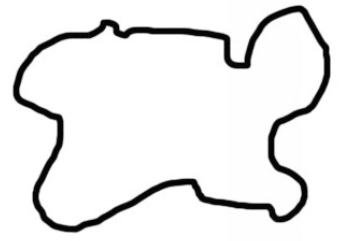
\includegraphics{img/fictional_country.png}

}

\caption{The outline of a fictional country.}

\end{figure}

Maybe the most simple, albeit naive approach would be to say that the
total area of this country can be modeled with a square. A square is a
very parsimonious model: in order to describe its area, only one
parameter is needed, its side length.

\begin{figure}

{\centering 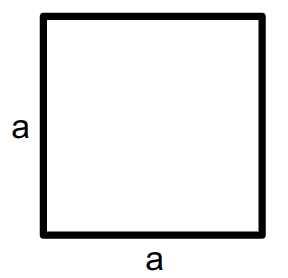
\includegraphics{img/square.png}

}

\caption{A square.}

\end{figure}

What's more, we can even give a precise mathematical formula for the
area of our fictional country under the square model:

\[M_1(a) = a^2\]

In Python code, we could express this model as the following function:

\begin{Shaded}
\begin{Highlighting}[]
\KeywordTok{def}\NormalTok{ square\_model(a):}
    \ControlFlowTok{return}\NormalTok{ a}\OperatorTok{**}\DecValTok{2}
\end{Highlighting}
\end{Shaded}

Of course, this is not a good model of the area of the country. But one
of the strengths of formal models is that they are unquivocal. There
might be situations, in which the rough estimate of the square model is
actually sufficient for our purpose. So why use a more complex model if
the simplest one does the job?

Most of the time, however, such a simplistic model will not suffice and
we need to invest brain power to come up with a better one.\footnote{`Better'
  means here that it is closer to the reality we actually want to
  describe, while at the same time being as simple as possible. This
  trade-off is usually called ``Occam's razor''. Google it!} The
following model is one way to improve upon our first mode:

\begin{figure}

{\centering 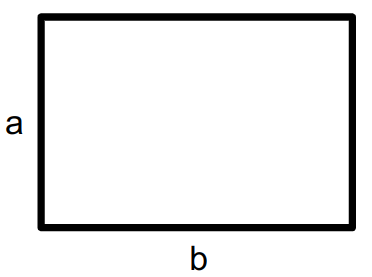
\includegraphics{img/rectangle.png}

}

\caption{A rectangle.}

\end{figure}

The shape of the rectangle seems to fit our country's outline better.
Hooray! As for the square model, we do have a mathematical formuly to
describe our rectangle model:

\[M_2(a,b) = a \cdot b\]

In Python code:

\begin{Shaded}
\begin{Highlighting}[]
\KeywordTok{def}\NormalTok{ rectangle(a,b):}
    \ControlFlowTok{return}\NormalTok{ a }\OperatorTok{*}\NormalTok{ b}
\end{Highlighting}
\end{Shaded}

But this improvement comes at a price: instead of having only one
parameter, \texttt{a}, we now have two, \texttt{a} and \texttt{b}. Our
model has instantly become twice as complex!

Modeling is at the core of social science and there are many good text
about this topic (McElreath, 2020; Smaldino, 2017; Smaldino, 2023). In
the humanities, there are fewer approaches taking modeling seriously,
but they are growing in number (Finkensiep et al., forthcoming;
Piotrowski, 2019).

\part{Foundations}

\hypertarget{sec-unbiased_transmission}{%
\chapter{Unbiased transmission}\label{sec-unbiased_transmission}}

What happens if people just blindly copy?

\hfill\break

\begin{tcolorbox}[enhanced jigsaw, arc=.35mm, colbacktitle=quarto-callout-note-color!10!white, colback=white, breakable, toprule=.15mm, title=\textcolor{quarto-callout-note-color}{\faInfo}\hspace{0.5em}{Note}, left=2mm, bottomtitle=1mm, toptitle=1mm, leftrule=.75mm, opacitybacktitle=0.6, titlerule=0mm, opacityback=0, rightrule=.15mm, bottomrule=.15mm, coltitle=black, colframe=quarto-callout-note-color-frame]

This chapter is based on ``Chapter 1: Unbiased transmission'' in Acerbi
et al. (2022).

\end{tcolorbox}

In this chapter, we introduce the most basic model for cultural
inheritance: unbiased transmission. This process quite literally
corresponds to randomly copying traits from previous generations,
without any further distinctions and constraints. While this is
obviously a too reductive model for how cultural transmission works, it
is ideally suited to get us started with the enterprise of modeling
evolutionary processes involving random variation.

First we import some modules.

\begin{Shaded}
\begin{Highlighting}[]
\ImportTok{import}\NormalTok{ numpy }\ImportTok{as}\NormalTok{ np}
\ImportTok{import}\NormalTok{ pandas }\ImportTok{as}\NormalTok{ pd}
\end{Highlighting}
\end{Shaded}

Because we will model evolutionary processes that are not strictly
deterministic, we need to simulate variations due to random change. For
this, we can use the \emph{default random number generator} from the
NumPy library and store it in the variable \texttt{rng}.

\begin{Shaded}
\begin{Highlighting}[]
\NormalTok{rng }\OperatorTok{=}\NormalTok{ np.random.default\_rng(seed}\OperatorTok{=}\DecValTok{42}\NormalTok{)}
\end{Highlighting}
\end{Shaded}

Next, we define some basic variables that we take into account for our
first model. We consider a population of \(N=100\) individuals as well
as a time-frame of \(t_{max}=100\) generations.

\hypertarget{creating-a-conceptual-understanding}{%
\section{Creating a conceptual
understanding}\label{creating-a-conceptual-understanding}}

It is a useful exercise to imagine first what we want to implement. This
way we can check whether we have a good conceptual understanding, which
will help us to write the code more clearly and make fewer mistakes. The
following figure shows in the upper panel a scenario, in which there is
a population of \texttt{N} individuals present in each generation. Those
individuals are uniquely characterized by one of two traits: whether
they like opera (salmon color) or not (grey). This visualization
captures all assumptions we make for our first model:

\begin{enumerate}
\def\labelenumi{\arabic{enumi}.}
\tightlist
\item
  The number of individuals per generation does not change.
\item
  Generations are disjunct, there is no overlap.
\item
  In the first generation, opera preference is randomly assigned to
  individuals.
\item
  In each subsequent generation, each individual randomly picks an
  `ancestor' from the previous generation and blindly copies that
  individual's preference for opera.
\end{enumerate}

The models throughout this book assume that invidivuals in one
generation learn from individuals of (only) the previous generation by
``picking'' an older individual and adopting its traits according to
some probabilistic rules built into the model. This means an arrow from
individual \texttt{n} in generation \texttt{t} to an individual
\texttt{m} in generation \texttt{t\ +\ 1} should be interpreted as:
``Individual \texttt{m} learns from individual \texttt{m}'' and not the
other way around (because information is flowing from generation
\texttt{t} to \texttt{t+1}).

\begin{figure}

{\centering 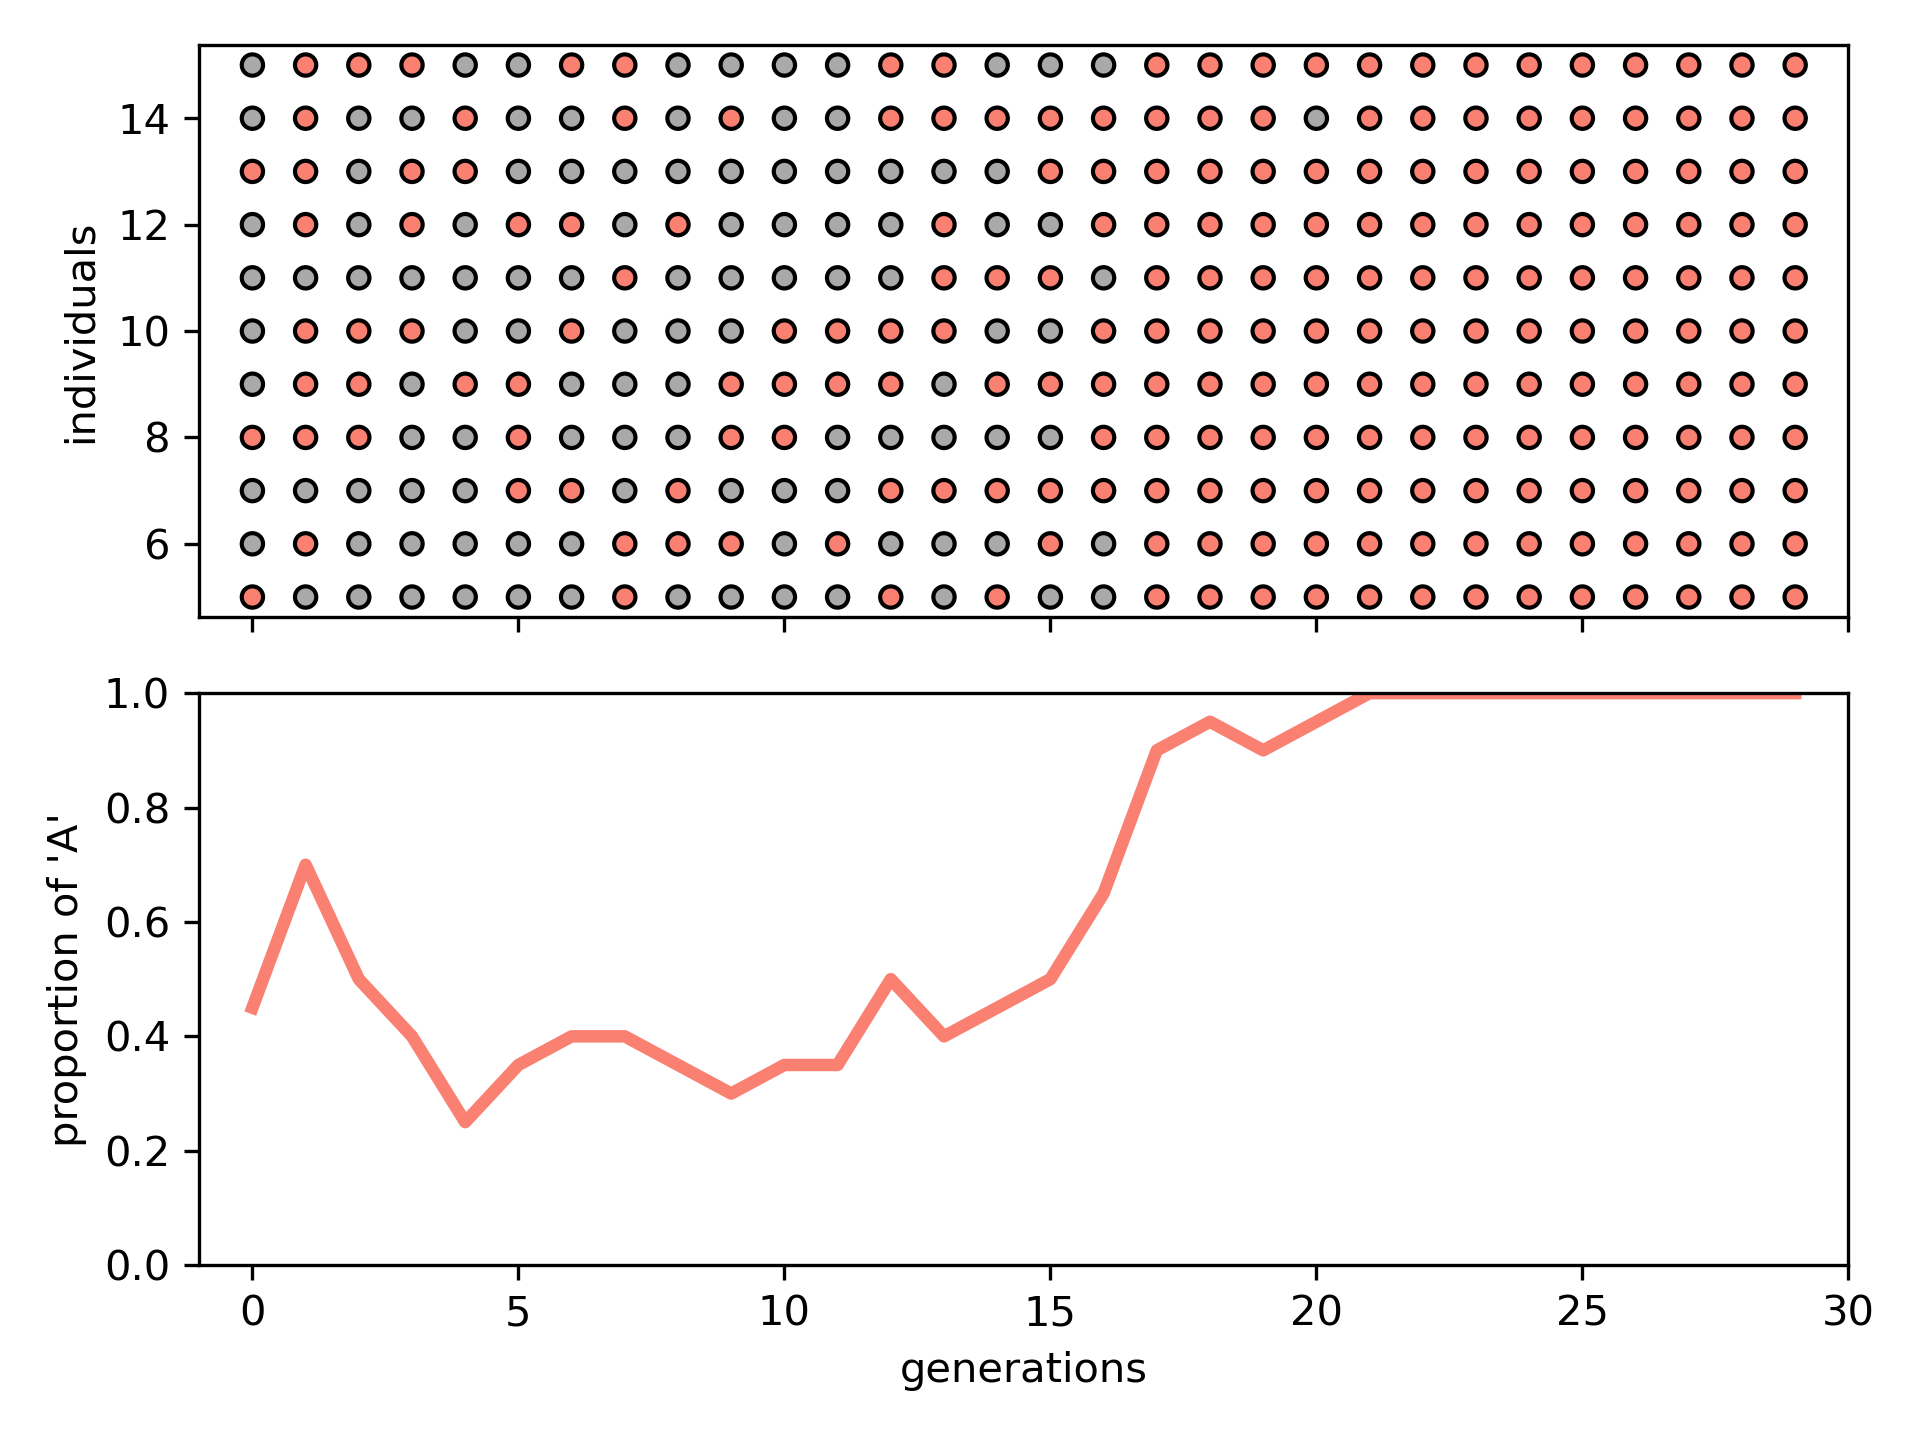
\includegraphics{img/chains.png}

}

\caption{A conceptual depiction of unbiased transmission.}

\end{figure}

The lower plot shows, at each time, point the percentage of individuals
having a preference for opera. A logical consequence of this process is
that each transmission chain (each sequence of directly connected
arrows) will pass through one and only one trait (color).

We can make further observations from this initial example. In the first
generation, there are two individuals who do like opera and three who
don't. In subsequent generations, the proporation of these two traits
changes. It is not \emph{monotonic} (it goes both up and down), as the
red line shows. But in the sixth generation, everything changes.
Individuals in the sixth generation \emph{could} inherit their trait
from the one individual in generation 5 that likes opera. But because
they randomly pick their ancestors, that individual is not among the
ancestors. Consequently, no individual in generation 6 likes opera. This
also means that, from now on, now one will ever like opera again. Opera
fans have become extinct.

We can see that transmission of information is still going on: there are
arrows between generations, so individuals still receive information
from the previous generation. But nothing changes. That means that we
\emph{do have} transmission of information, but we would not anymore
speak of it as \emph{cultural evolution}, since the first fundamental
criterion (see Chapter X), variation, is not fulfilled.

Note also, that some `traditions' are likewise not continued. For
example, following the transmission chain of individual 0 in the first
generation to individual 2 in the second generation to individual 3 in
the third generation, we see that this latter individual is not picked
as an ancestor by anyone from the next generation. This individual (and
all of its ancestors) have no more impact on future generations.
Importantly, however, we are not interested in individual fates, but
rather in population-level statistics. That is why the lower plot only
traces the proportion of individuals having a preference for opera.

\hypertarget{simulating-a-population}{%
\section{Simulating a population}\label{simulating-a-population}}

With this conceptual understanding in mind, we will now look at how we
can reproduce this model of unbiased transmission. Since we are assuming
that new individuals randomly pick an ancestor, we should not assume
that our results will be exactly the same as above, but they should
nonetheless be qualitatively similar.

\begin{Shaded}
\begin{Highlighting}[]
\NormalTok{N }\OperatorTok{=} \DecValTok{100}
\NormalTok{t\_max }\OperatorTok{=} \DecValTok{100}
\end{Highlighting}
\end{Shaded}

\begin{tcolorbox}[enhanced jigsaw, arc=.35mm, colbacktitle=quarto-callout-note-color!10!white, colback=white, breakable, toprule=.15mm, title=\textcolor{quarto-callout-note-color}{\faInfo}\hspace{0.5em}{Note}, left=2mm, bottomtitle=1mm, toptitle=1mm, leftrule=.75mm, opacitybacktitle=0.6, titlerule=0mm, opacityback=0, rightrule=.15mm, bottomrule=.15mm, coltitle=black, colframe=quarto-callout-note-color-frame]

In general, we use the variable \texttt{t} to designate generation
counts.

\end{tcolorbox}

Now we create a variable \texttt{population} that will store the data
about our simulated population. This population has either of two traits
\texttt{"A"} and \texttt{"B"}, with a certain probability. We store all
of this in a so-called `data frame', which is a somewhat fancy,
Pandas-specific term for a table.

\begin{Shaded}
\begin{Highlighting}[]
\NormalTok{population }\OperatorTok{=}\NormalTok{ pd.DataFrame(}
\NormalTok{    \{}\StringTok{"trait"}\NormalTok{: rng.choice([}\StringTok{"A"}\NormalTok{, }\StringTok{"B"}\NormalTok{], size}\OperatorTok{=}\NormalTok{N, replace}\OperatorTok{=}\VariableTok{True}\NormalTok{)\}}
\NormalTok{)}
\end{Highlighting}
\end{Shaded}

Let's take this code apart to understand it better. From the Pandas
library, which we imported as the alias \texttt{pd}, we create a
\texttt{DataFrame} object. The data contained in this the data frame
\texttt{population} is specified via a dictionary that has
\texttt{"trait"} as its key and a fairly complex expression starting
with the random number generator \texttt{rng} as its value. What this
value says is, from the list \texttt{{[}"A",\ "B"{]}} choose randomly
\texttt{N} instances with replacement (if \texttt{replace} were set to
\texttt{False}, we could at most sample 2 values from the list). So, the
data frame \texttt{population} should contain 100 randomly sampled
values of A's and B's. Let's confirm this:

\begin{Shaded}
\begin{Highlighting}[]
\NormalTok{population.head()}
\end{Highlighting}
\end{Shaded}

\begin{tabular}{ll}
\toprule
{} & trait \\
\midrule
0 &     A \\
1 &     B \\
2 &     B \\
3 &     A \\
4 &     A \\
\bottomrule
\end{tabular}

As you can see, \texttt{population} stores a table (many of the 100 rows
are omitted here for display reasons) and a single column called
`trait'. The \texttt{.head()} method appended to the \texttt{population}
data frame shows restricts the output to only the first 5 rows (0
through 4). Each row in the `trait' column contains either the value A
or B. To the left of the data frame you can see the numbers of rows
explicitly spelled out. This is called the data frame's \emph{index}.

\begin{tcolorbox}[enhanced jigsaw, arc=.35mm, colbacktitle=quarto-callout-note-color!10!white, colback=white, breakable, toprule=.15mm, title=\textcolor{quarto-callout-note-color}{\faInfo}\hspace{0.5em}{Note}, left=2mm, bottomtitle=1mm, toptitle=1mm, leftrule=.75mm, opacitybacktitle=0.6, titlerule=0mm, opacityback=0, rightrule=.15mm, bottomrule=.15mm, coltitle=black, colframe=quarto-callout-note-color-frame]

A and B are just placeholder names for any of two mutually exclusive
cultural traits. These could be, for example, preference for red over
white whine (ignoring people who like rosé as well as people who have no
preference). You see already here that this is a massive
oversimplification of actual taste preferences. The point here is not to
construct a plausible model but rather to gradually build up a simple
one in order to understand well its inner workings.

It will help to pause for a moment and to think of other examples that
``A'' and ``B'' could stand for. Can you come up with a music-related
one?

\end{tcolorbox}

For instance, we could say that the mutually exclusive traits ``A'' and
``B'' correspond to ``Individual likes opera'' and ``Individual doesn't
like opera''. People are often opinionated about opera, so we will stick
to this example for the remainder of this part of the book. But be
encouraged to try to transfer the following to different hypothetical
scenarios.

\begin{figure}

{\centering 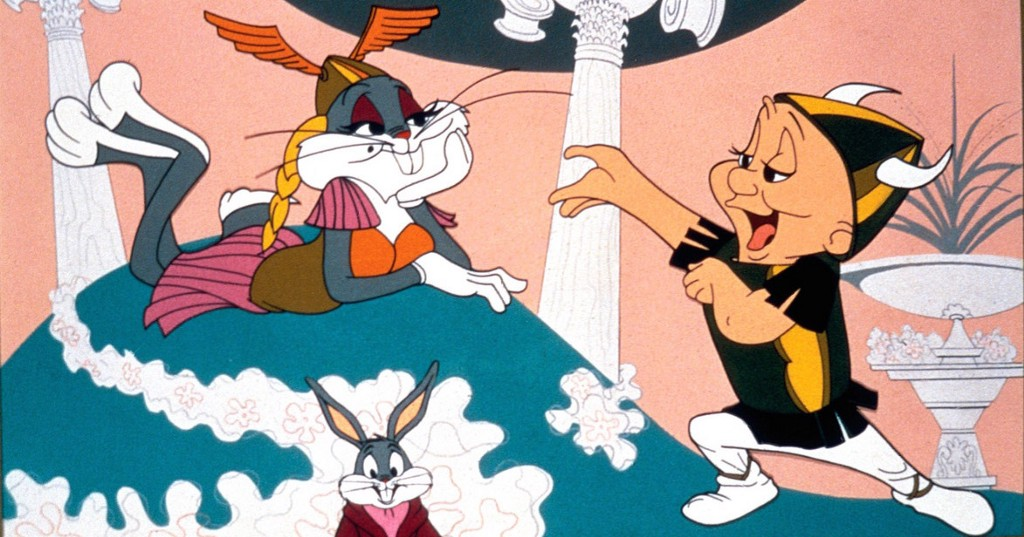
\includegraphics{img/opera.jpeg}

}

\caption{Scene from
\href{https://en.wikipedia.org/wiki/What\%27s_Opera,_Doc}{``What's
opera, doc?''} (1957).}

\end{figure}

Back to our artificial population. We can count the number of A's and
B's amongst the individuals as follows:

\begin{Shaded}
\begin{Highlighting}[]
\NormalTok{population[}\StringTok{"trait"}\NormalTok{].value\_counts()}
\end{Highlighting}
\end{Shaded}

\begin{tabular}{lr}
\toprule
{} &  trait \\
\midrule
B &     52 \\
A &     48 \\
\bottomrule
\end{tabular}

You can read the above code as ``From the population table, select the
`trait' colum and count its values.''. Since there were only two values
to sample from and they were randomly (uniformly) sampled, the number of
A's and the number of B's should be approximately equal. We can obtain
their relative frequencies by adding setting the \texttt{normalize}
keyword to \texttt{True}:

\begin{Shaded}
\begin{Highlighting}[]
\NormalTok{population[}\StringTok{"trait"}\NormalTok{].value\_counts(normalize}\OperatorTok{=}\VariableTok{True}\NormalTok{)}
\end{Highlighting}
\end{Shaded}

\begin{tabular}{lr}
\toprule
{} &  trait \\
\midrule
B &   0.52 \\
A &   0.48 \\
\bottomrule
\end{tabular}

\hypertarget{tracing-cultural-change}{%
\section{Tracing cultural change}\label{tracing-cultural-change}}

We now create a second data frame \texttt{output} in which we will store
the output of our model. This data frame has two columns:
\texttt{generation}, which is the number of the simulated generation,
and \texttt{p} which stands for ``the probability of an individual of
having trait A''.

\begin{Shaded}
\begin{Highlighting}[]
\NormalTok{output }\OperatorTok{=}\NormalTok{ pd.DataFrame(}
\NormalTok{    \{}
        \StringTok{"generation"}\NormalTok{: np.arange(t\_max, dtype}\OperatorTok{=}\BuiltInTok{int}\NormalTok{), }
        \StringTok{"p"}\NormalTok{: [np.nan] }\OperatorTok{*}\NormalTok{ t\_max }
\NormalTok{    \}}
\NormalTok{)}
\end{Highlighting}
\end{Shaded}

The \texttt{generation} column contains all numbers from \texttt{0} to
\texttt{t\_max\ -\ 1}. Because we count the numbers of generations
(rather than assuming a time-continuous process), we specified that
numbers in this column have to be intergers (\texttt{dtype=int}). The
values for the \texttt{p} column must look cryptic. It literally says:
put the \texttt{np.nan} value \texttt{t\_max} times into the \texttt{p}
colum. \texttt{np.nan} stands for ``not a number'' (from the NumPy
library), since we haven't assigned any values to this probability yet.

\begin{Shaded}
\begin{Highlighting}[]
\NormalTok{output.head()}
\end{Highlighting}
\end{Shaded}

\begin{tabular}{lrr}
\toprule
{} &  generation &   p \\
\midrule
0 &           0 & NaN \\
1 &           1 & NaN \\
2 &           2 & NaN \\
3 &           3 & NaN \\
4 &           4 & NaN \\
\bottomrule
\end{tabular}

Don't worry that both the index and the `generation' column contain all
numbers from 0 to 99. We need this later when things become more
involved.

As the saying goes, from nothing comes nothing, so we have to start
somewhere, meaning that we need to assume that the initial probability
of having trait A in our population is an actual number. The most
sensible thing is to start with the proportions of A and B in our
sampled population as a starting value.

So, we approximate the probability of an individual having trait A with
the relative frequency of trait A in the population:

\begin{Shaded}
\begin{Highlighting}[]
\NormalTok{population[}\StringTok{"trait"}\NormalTok{].value\_counts(normalize}\OperatorTok{=}\VariableTok{True}\NormalTok{)[}\StringTok{"A"}\NormalTok{]}
\end{Highlighting}
\end{Shaded}

\begin{verbatim}
0.48
\end{verbatim}

You already know this code from above, we just added the
\texttt{{[}"A"{]}} part at the end to select only the relative
frequencies of trait A. We want to set this as the value of \texttt{p}
of the first generation. This can be achieved with the \texttt{.loc}
(location) method:

\begin{Shaded}
\begin{Highlighting}[]
\NormalTok{output.loc[}\DecValTok{0}\NormalTok{, }\StringTok{"p"}\NormalTok{] }\OperatorTok{=}\NormalTok{ population[}\StringTok{"trait"}\NormalTok{].value\_counts(normalize}\OperatorTok{=}\VariableTok{True}\NormalTok{)[}\StringTok{"A"}\NormalTok{]}
\end{Highlighting}
\end{Shaded}

In words, this reads: ``Set location 0 (first row) in the \texttt{p}
column of the \texttt{output} data frame to the relative frequency of
the trait `A' in the population.''

\hypertarget{iterating-over-generations}{%
\section{Iterating over generations}\label{iterating-over-generations}}

Recall that we are trying to observe cultural change over the course of
\texttt{t\_max\ =\ 100} generations. We thus simply repeat what we just
did for the first generation: based on the relative frequencies of A's
and B's in the previous generation, we sample the traits of 100 new
individuals for the next generation.

\begin{Shaded}
\begin{Highlighting}[]
\ControlFlowTok{for}\NormalTok{ t }\KeywordTok{in} \BuiltInTok{range}\NormalTok{(}\DecValTok{1}\NormalTok{, t\_max):}
    \CommentTok{\# Copy the population data frame to \textasciigrave{}previous\_population\textasciigrave{}}
\NormalTok{    previous\_population }\OperatorTok{=}\NormalTok{ population.copy()}
  
    \CommentTok{\# Randomly copy from previous generation\textquotesingle{}s individuals}
\NormalTok{    new\_population }\OperatorTok{=}\NormalTok{ previous\_population[}\StringTok{"trait"}\NormalTok{].sample(N, replace}\OperatorTok{=}\VariableTok{True}\NormalTok{).to\_frame()}
    
    \CommentTok{\# Get p and put it into the output slot for this generation t}
\NormalTok{    output.loc[t, }\StringTok{"p"}\NormalTok{] }\OperatorTok{=}\NormalTok{ new\_population[ new\_population[}\StringTok{"trait"}\NormalTok{] }\OperatorTok{==} \StringTok{"A"}\NormalTok{].shape[}\DecValTok{0}\NormalTok{] }\OperatorTok{/}\NormalTok{ N}
\end{Highlighting}
\end{Shaded}

This procedure assignes a probability of having trait ``A'' for each
generation (each row of the \texttt{p} colum is filled now):

\begin{Shaded}
\begin{Highlighting}[]
\NormalTok{output.head()}
\end{Highlighting}
\end{Shaded}

\begin{tabular}{lrr}
\toprule
{} &  generation &     p \\
\midrule
0 &           0 &  0.48 \\
1 &           1 &  0.49 \\
2 &           2 &  0.44 \\
3 &           3 &  0.52 \\
4 &           4 &  0.45 \\
\bottomrule
\end{tabular}

To make things easier, we wrap the above code in a function that we'll
call \texttt{unbiased\_transmission} that can take different values for
the population size \texttt{N} and number of generations \texttt{t\_max}
as parameters. The code below is exactly the same as above.

\begin{Shaded}
\begin{Highlighting}[]
\KeywordTok{def}\NormalTok{ unbiased\_transmission\_1(N, t\_max):}
\NormalTok{    population }\OperatorTok{=}\NormalTok{ pd.DataFrame(\{}\StringTok{"trait"}\NormalTok{: rng.choice([}\StringTok{"A"}\NormalTok{, }\StringTok{"B"}\NormalTok{], size}\OperatorTok{=}\NormalTok{N, replace}\OperatorTok{=}\VariableTok{True}\NormalTok{)\})}

\NormalTok{    output }\OperatorTok{=}\NormalTok{ pd.DataFrame(\{}\StringTok{"generation"}\NormalTok{: np.arange(t\_max, dtype}\OperatorTok{=}\BuiltInTok{int}\NormalTok{), }\StringTok{"p"}\NormalTok{: [np.nan] }\OperatorTok{*}\NormalTok{ t\_max \})}

\NormalTok{    output.loc[}\DecValTok{0}\NormalTok{, }\StringTok{"p"}\NormalTok{] }\OperatorTok{=}\NormalTok{ population[ population[}\StringTok{"trait"}\NormalTok{] }\OperatorTok{==} \StringTok{"A"}\NormalTok{].shape[}\DecValTok{0}\NormalTok{] }\OperatorTok{/}\NormalTok{ N}

    \ControlFlowTok{for}\NormalTok{ t }\KeywordTok{in} \BuiltInTok{range}\NormalTok{(}\DecValTok{1}\NormalTok{, t\_max):}
        \CommentTok{\# Copy the population tibble to previous\_population tibble}
\NormalTok{        previous\_population }\OperatorTok{=}\NormalTok{ population.copy()}
    
        \CommentTok{\# Randomly copy from previous generation\textquotesingle{}s individuals}
\NormalTok{        new\_population }\OperatorTok{=}\NormalTok{ previous\_population[}\StringTok{"trait"}\NormalTok{].sample(N, replace}\OperatorTok{=}\VariableTok{True}\NormalTok{).to\_frame()}
        
        \CommentTok{\# Get p and put it into the output slot for this generation t}
\NormalTok{        output.loc[t, }\StringTok{"p"}\NormalTok{] }\OperatorTok{=}\NormalTok{ new\_population[ new\_population[}\StringTok{"trait"}\NormalTok{] }\OperatorTok{==} \StringTok{"A"}\NormalTok{].shape[}\DecValTok{0}\NormalTok{] }\OperatorTok{/}\NormalTok{ N}
    
    \ControlFlowTok{return}\NormalTok{ output}
\end{Highlighting}
\end{Shaded}

\begin{Shaded}
\begin{Highlighting}[]
\NormalTok{data\_model }\OperatorTok{=}\NormalTok{ unbiased\_transmission\_1(N}\OperatorTok{=}\DecValTok{100}\NormalTok{, t\_max}\OperatorTok{=}\DecValTok{200}\NormalTok{)}
\end{Highlighting}
\end{Shaded}

\begin{Shaded}
\begin{Highlighting}[]
\KeywordTok{def}\NormalTok{ plot\_single\_run(data\_model):}
\NormalTok{    data\_model[}\StringTok{"p"}\NormalTok{].plot(ylim}\OperatorTok{=}\NormalTok{(}\DecValTok{0}\NormalTok{,}\DecValTok{1}\NormalTok{))}
\end{Highlighting}
\end{Shaded}

\begin{Shaded}
\begin{Highlighting}[]
\NormalTok{plot\_single\_run(data\_model)}
\end{Highlighting}
\end{Shaded}

\begin{figure}[H]

{\centering 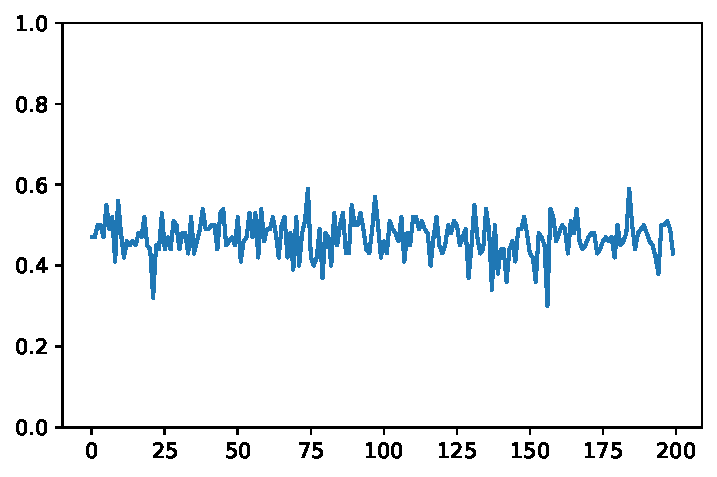
\includegraphics{chapter03_files/figure-pdf/cell-18-output-1.pdf}

}

\caption{Single run of the unbiased transmission model for a population
of \(N=100\) individuals and \(t_{max}=200\) generations.}

\end{figure}

\begin{Shaded}
\begin{Highlighting}[]
\NormalTok{data\_model }\OperatorTok{=}\NormalTok{ unbiased\_transmission\_1(N}\OperatorTok{=}\DecValTok{10\_000}\NormalTok{, t\_max}\OperatorTok{=}\DecValTok{200}\NormalTok{)}
\end{Highlighting}
\end{Shaded}

\begin{Shaded}
\begin{Highlighting}[]
\NormalTok{plot\_single\_run(data\_model)}
\end{Highlighting}
\end{Shaded}

\begin{figure}[H]

{\centering 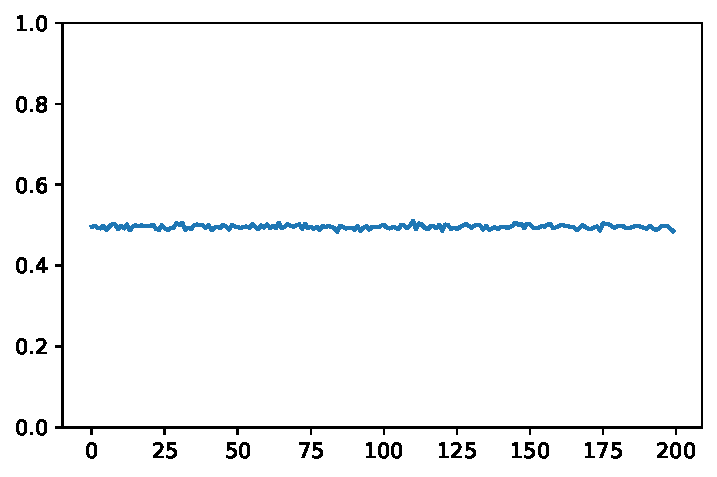
\includegraphics{chapter03_files/figure-pdf/cell-20-output-1.pdf}

}

\caption{Single run of the unbiased transmission model for a population
of \(N=10,000\) individuals and \(t_{max}=200\) generations.}

\end{figure}

Now, let's adapt the code somewhat.

\begin{Shaded}
\begin{Highlighting}[]
\KeywordTok{def}\NormalTok{ unbiased\_transmission\_2(N, t\_max, r\_max):}
\NormalTok{    output }\OperatorTok{=}\NormalTok{ pd.DataFrame(\{}
        \StringTok{"generation"}\NormalTok{ : np.tile(np.arange(t\_max), r\_max),}
        \StringTok{"p"}\NormalTok{ : [ np.nan ] }\OperatorTok{*}\NormalTok{ t\_max }\OperatorTok{*}\NormalTok{ r\_max,}
        \StringTok{"run"}\NormalTok{ : np.repeat(np.arange(r\_max), t\_max)}
\NormalTok{    \})}

    \ControlFlowTok{for}\NormalTok{ r }\KeywordTok{in} \BuiltInTok{range}\NormalTok{(r\_max):}
        \CommentTok{\# Create first generation}
\NormalTok{        population }\OperatorTok{=}\NormalTok{ pd.DataFrame(\{}\StringTok{"trait"}\NormalTok{: rng.choice([}\StringTok{"A"}\NormalTok{, }\StringTok{"B"}\NormalTok{], size}\OperatorTok{=}\NormalTok{N, replace}\OperatorTok{=}\VariableTok{True}\NormalTok{)\})}

        \CommentTok{\# Add first generation\textquotesingle{}s p for run r}
\NormalTok{        output.loc[ r }\OperatorTok{*}\NormalTok{ t\_max, }\StringTok{"p"}\NormalTok{] }\OperatorTok{=}\NormalTok{ population[ population[}\StringTok{"trait"}\NormalTok{] }\OperatorTok{==} \StringTok{"A"}\NormalTok{ ].shape[}\DecValTok{0}\NormalTok{] }\OperatorTok{/}\NormalTok{ N}

        \CommentTok{\# For each generation }
        \ControlFlowTok{for}\NormalTok{ t }\KeywordTok{in} \BuiltInTok{range}\NormalTok{(}\DecValTok{1}\NormalTok{,t\_max):}
            \CommentTok{\# Copy individuals to previous\_population DataFrame}
\NormalTok{            previous\_population }\OperatorTok{=}\NormalTok{ population.copy()}

            \CommentTok{\# Randomly compy from previous generation }
\NormalTok{            population }\OperatorTok{=}\NormalTok{ population[}\StringTok{"trait"}\NormalTok{].sample(N, replace}\OperatorTok{=}\VariableTok{True}\NormalTok{).to\_frame()}

            \CommentTok{\# Get p and put it into output slot for this generation t and run r}
\NormalTok{            output.loc[r }\OperatorTok{*}\NormalTok{ t\_max }\OperatorTok{+}\NormalTok{ t, }\StringTok{"p"}\NormalTok{] }\OperatorTok{=}\NormalTok{ population[ population[}\StringTok{"trait"}\NormalTok{] }\OperatorTok{==} \StringTok{"A"}\NormalTok{ ].shape[}\DecValTok{0}\NormalTok{] }\OperatorTok{/}\NormalTok{ N}

    \ControlFlowTok{return}\NormalTok{ output}
\end{Highlighting}
\end{Shaded}

\begin{Shaded}
\begin{Highlighting}[]
\NormalTok{unbiased\_transmission\_2(}\DecValTok{100}\NormalTok{, }\DecValTok{100}\NormalTok{, }\DecValTok{3}\NormalTok{).head()}
\end{Highlighting}
\end{Shaded}

\begin{tabular}{lrrr}
\toprule
{} &  generation &     p &  run \\
\midrule
0 &           0 &  0.45 &    0 \\
1 &           1 &  0.48 &    0 \\
2 &           2 &  0.46 &    0 \\
3 &           3 &  0.46 &    0 \\
4 &           4 &  0.44 &    0 \\
\bottomrule
\end{tabular}

\begin{tcolorbox}[enhanced jigsaw, arc=.35mm, colbacktitle=quarto-callout-tip-color!10!white, colback=white, breakable, toprule=.15mm, title=\textcolor{quarto-callout-tip-color}{\faLightbulb}\hspace{0.5em}{Tip}, left=2mm, bottomtitle=1mm, toptitle=1mm, leftrule=.75mm, opacitybacktitle=0.6, titlerule=0mm, opacityback=0, rightrule=.15mm, bottomrule=.15mm, coltitle=black, colframe=quarto-callout-tip-color-frame]

Why could we append \texttt{.head()} to the
\texttt{unbiased\_transmission\_2} function?

\end{tcolorbox}

\begin{Shaded}
\begin{Highlighting}[]
\NormalTok{data\_model }\OperatorTok{=}\NormalTok{ unbiased\_transmission\_2(N}\OperatorTok{=}\DecValTok{100}\NormalTok{, t\_max}\OperatorTok{=}\DecValTok{200}\NormalTok{, r\_max}\OperatorTok{=}\DecValTok{5}\NormalTok{)}
\end{Highlighting}
\end{Shaded}

\begin{Shaded}
\begin{Highlighting}[]
\KeywordTok{def}\NormalTok{ plot\_multiple\_runs(data\_model):}
\NormalTok{    groups }\OperatorTok{=}\NormalTok{ data\_model.groupby(}\StringTok{"run"}\NormalTok{)}
    \ControlFlowTok{for}\NormalTok{ \_, g }\KeywordTok{in}\NormalTok{ groups:}
\NormalTok{        g.index }\OperatorTok{=}\NormalTok{ g[}\StringTok{"generation"}\NormalTok{]}
\NormalTok{        g[}\StringTok{"p"}\NormalTok{].plot(lw}\OperatorTok{=}\FloatTok{.5}\NormalTok{, ylim}\OperatorTok{=}\NormalTok{(}\DecValTok{0}\NormalTok{,}\DecValTok{1}\NormalTok{))}

\NormalTok{    data\_model.groupby(}\StringTok{"generation"}\NormalTok{)[}\StringTok{"p"}\NormalTok{].mean().plot(c}\OperatorTok{=}\StringTok{"k"}\NormalTok{, lw}\OperatorTok{=}\StringTok{"1"}\NormalTok{)}
\end{Highlighting}
\end{Shaded}

\begin{Shaded}
\begin{Highlighting}[]
\NormalTok{plot\_multiple\_runs(data\_model)}
\end{Highlighting}
\end{Shaded}

\begin{figure}[H]

{\centering 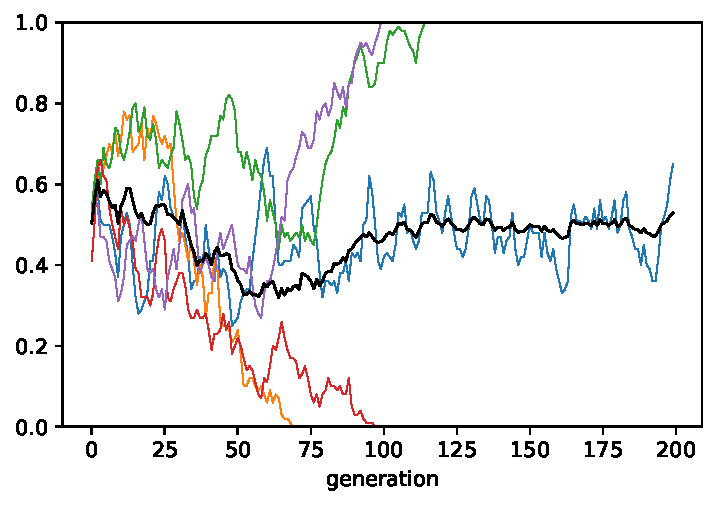
\includegraphics{chapter03_files/figure-pdf/cell-25-output-1.pdf}

}

\caption{Multiple runs of the unbiased transmission model for a
population of \(N=100\) individuals, with average (black line).}

\end{figure}

\begin{Shaded}
\begin{Highlighting}[]
\NormalTok{data\_model }\OperatorTok{=}\NormalTok{ unbiased\_transmission\_2(N}\OperatorTok{=}\DecValTok{10\_000}\NormalTok{, t\_max}\OperatorTok{=}\DecValTok{200}\NormalTok{, r\_max}\OperatorTok{=}\DecValTok{5}\NormalTok{)}
\end{Highlighting}
\end{Shaded}

\begin{Shaded}
\begin{Highlighting}[]
\NormalTok{plot\_multiple\_runs(data\_model)}
\end{Highlighting}
\end{Shaded}

\begin{figure}[H]

{\centering 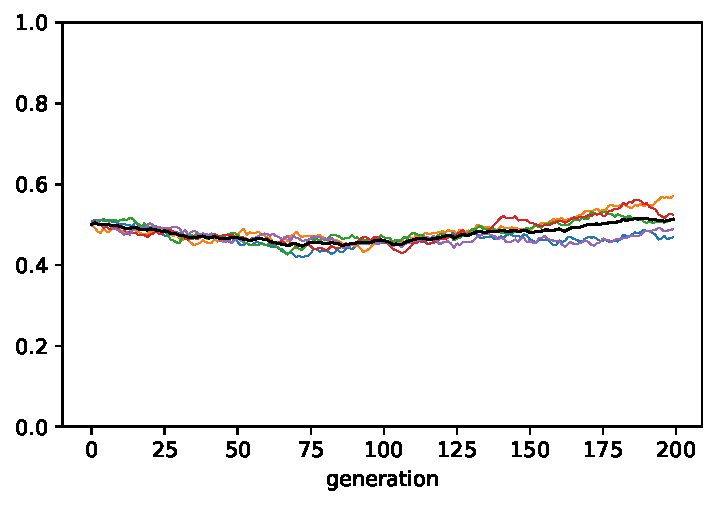
\includegraphics{chapter03_files/figure-pdf/cell-27-output-1.pdf}

}

\caption{Multiple runs of the unbiased transmission model for a
population of \(N=10,000\) individuals, with average (black line).}

\end{figure}

\begin{Shaded}
\begin{Highlighting}[]
\KeywordTok{def}\NormalTok{ unbiased\_transmission\_3(N, p\_0, t\_max, r\_max):}
\NormalTok{    output }\OperatorTok{=}\NormalTok{ pd.DataFrame(\{}
        \StringTok{"generation"}\NormalTok{ : np.tile(np.arange(t\_max), r\_max),}
        \StringTok{"p"}\NormalTok{ : [ np.nan ] }\OperatorTok{*}\NormalTok{ t\_max }\OperatorTok{*}\NormalTok{ r\_max,}
        \StringTok{"run"}\NormalTok{ : np.repeat(np.arange(r\_max), t\_max)}
\NormalTok{    \})}

    \ControlFlowTok{for}\NormalTok{ r }\KeywordTok{in} \BuiltInTok{range}\NormalTok{(r\_max):}
        \CommentTok{\# Create first generation}
\NormalTok{        population }\OperatorTok{=}\NormalTok{ pd.DataFrame(\{}\StringTok{"trait"}\NormalTok{: rng.choice([}\StringTok{"A"}\NormalTok{, }\StringTok{"B"}\NormalTok{], size}\OperatorTok{=}\NormalTok{N, replace}\OperatorTok{=}\VariableTok{True}\NormalTok{, p}\OperatorTok{=}\NormalTok{[p\_0, }\DecValTok{1} \OperatorTok{{-}}\NormalTok{ p\_0])\})}

        \CommentTok{\# Add first generation\textquotesingle{}s p for run r}
\NormalTok{        output.loc[ r }\OperatorTok{*}\NormalTok{ t\_max, }\StringTok{"p"}\NormalTok{] }\OperatorTok{=}\NormalTok{ population[ population[}\StringTok{"trait"}\NormalTok{] }\OperatorTok{==} \StringTok{"A"}\NormalTok{ ].shape[}\DecValTok{0}\NormalTok{] }\OperatorTok{/}\NormalTok{ N}

        \CommentTok{\# For each generation }
        \ControlFlowTok{for}\NormalTok{ t }\KeywordTok{in} \BuiltInTok{range}\NormalTok{(}\DecValTok{1}\NormalTok{,t\_max):}
            \CommentTok{\# Copy individuals to previous\_population DataFrame}
\NormalTok{            previous\_population }\OperatorTok{=}\NormalTok{ population}

            \CommentTok{\# Randomly compy from previous generation }
\NormalTok{            population }\OperatorTok{=}\NormalTok{ population[}\StringTok{"trait"}\NormalTok{].sample(N, replace}\OperatorTok{=}\VariableTok{True}\NormalTok{).to\_frame()}

            \CommentTok{\# Get p and put it into output slot for this generation t and run r}
\NormalTok{            output.loc[r }\OperatorTok{*}\NormalTok{ t\_max }\OperatorTok{+}\NormalTok{ t, }\StringTok{"p"}\NormalTok{] }\OperatorTok{=}\NormalTok{ population[ population[}\StringTok{"trait"}\NormalTok{] }\OperatorTok{==} \StringTok{"A"}\NormalTok{ ].shape[}\DecValTok{0}\NormalTok{] }\OperatorTok{/}\NormalTok{ N}

    \ControlFlowTok{return}\NormalTok{ output}
\end{Highlighting}
\end{Shaded}

\begin{Shaded}
\begin{Highlighting}[]
\NormalTok{data\_model }\OperatorTok{=}\NormalTok{ unbiased\_transmission\_3(}\DecValTok{10\_000}\NormalTok{, p\_0}\OperatorTok{=}\FloatTok{.2}\NormalTok{, t\_max}\OperatorTok{=}\DecValTok{200}\NormalTok{, r\_max}\OperatorTok{=}\DecValTok{5}\NormalTok{)}
\NormalTok{plot\_multiple\_runs(data\_model)}
\end{Highlighting}
\end{Shaded}

\begin{figure}[H]

{\centering 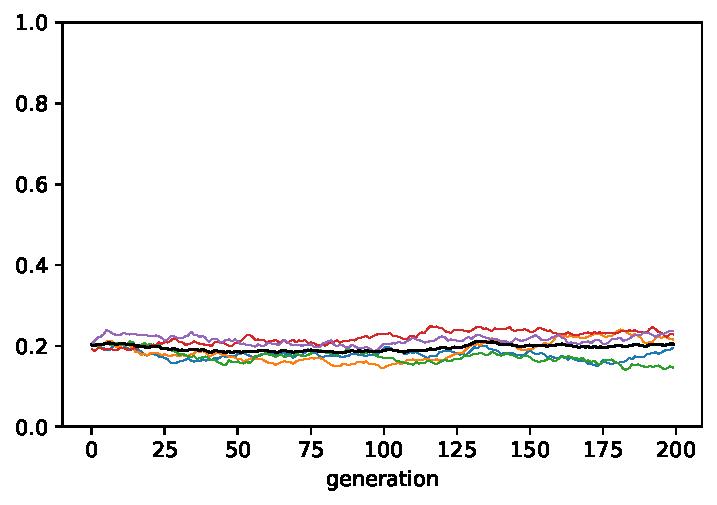
\includegraphics{chapter03_files/figure-pdf/cell-29-output-1.pdf}

}

\end{figure}

\hypertarget{sec-unbiased_biased_mutation}{%
\chapter{Unbiased mutation}\label{sec-unbiased_biased_mutation}}

\begin{tcolorbox}[enhanced jigsaw, arc=.35mm, colbacktitle=quarto-callout-note-color!10!white, colback=white, breakable, toprule=.15mm, title=\textcolor{quarto-callout-note-color}{\faInfo}\hspace{0.5em}{Note}, left=2mm, bottomtitle=1mm, toptitle=1mm, leftrule=.75mm, opacitybacktitle=0.6, titlerule=0mm, opacityback=0, rightrule=.15mm, bottomrule=.15mm, coltitle=black, colframe=quarto-callout-note-color-frame]

This chapter is based on ``Chapter 2: Unbiased and biased mutation'' in
Acerbi et al. (2022).

\end{tcolorbox}

\begin{Shaded}
\begin{Highlighting}[]
\ImportTok{import}\NormalTok{ numpy }\ImportTok{as}\NormalTok{ np}
\NormalTok{rng }\OperatorTok{=}\NormalTok{ np.random.default\_rng()}

\ImportTok{import}\NormalTok{ pandas }\ImportTok{as}\NormalTok{ pd}
\end{Highlighting}
\end{Shaded}

\begin{Shaded}
\begin{Highlighting}[]
\KeywordTok{def}\NormalTok{ unbiased\_mutation(N, mu, p\_0, t\_max, r\_max):}
    \CommentTok{\# Create an output DataFrame}
\NormalTok{    output }\OperatorTok{=}\NormalTok{ pd.DataFrame(\{}
        \StringTok{"generation"}\NormalTok{ : np.tile(np.arange(t\_max), r\_max),}
        \StringTok{"p"}\NormalTok{ : [ np.nan ] }\OperatorTok{*}\NormalTok{ t\_max }\OperatorTok{*}\NormalTok{ r\_max,}
        \StringTok{"run"}\NormalTok{ : np.repeat(np.arange(r\_max), t\_max)}
\NormalTok{    \})}

    \ControlFlowTok{for}\NormalTok{ r }\KeywordTok{in} \BuiltInTok{range}\NormalTok{(r\_max):}
        \CommentTok{\# Create first generation}
\NormalTok{        population }\OperatorTok{=}\NormalTok{ pd.DataFrame(\{}\StringTok{"trait"}\NormalTok{: rng.choice([}\StringTok{"A"}\NormalTok{, }\StringTok{"B"}\NormalTok{], size}\OperatorTok{=}\NormalTok{N, replace}\OperatorTok{=}\VariableTok{True}\NormalTok{, p}\OperatorTok{=}\NormalTok{[p\_0, }\DecValTok{1} \OperatorTok{{-}}\NormalTok{ p\_0])\})}

        \CommentTok{\# Add first generation\textquotesingle{}s p for run r}
\NormalTok{        output.loc[ r }\OperatorTok{*}\NormalTok{ t\_max, }\StringTok{"p"}\NormalTok{] }\OperatorTok{=}\NormalTok{ population[ population[}\StringTok{"trait"}\NormalTok{] }\OperatorTok{==} \StringTok{"A"}\NormalTok{ ].shape[}\DecValTok{0}\NormalTok{] }\OperatorTok{/}\NormalTok{ N}

        \CommentTok{\# For each generation }
        \ControlFlowTok{for}\NormalTok{ t }\KeywordTok{in} \BuiltInTok{range}\NormalTok{(}\DecValTok{1}\NormalTok{,t\_max):}
            \CommentTok{\# Copy individuals to previous\_population DataFrame}
\NormalTok{            previous\_population }\OperatorTok{=}\NormalTok{ population.copy()}
            
            \CommentTok{\# Determine "mutant" individuals}
\NormalTok{            mutate }\OperatorTok{=}\NormalTok{ rng.choice([}\VariableTok{True}\NormalTok{, }\VariableTok{False}\NormalTok{], size}\OperatorTok{=}\NormalTok{N, p}\OperatorTok{=}\NormalTok{[mu, }\DecValTok{1}\OperatorTok{{-}}\NormalTok{mu], replace}\OperatorTok{=}\VariableTok{True}\NormalTok{)}

            \CommentTok{\# }\AlertTok{TODO}\CommentTok{: Something is off here! Changing the order of the conditions affects}
            \CommentTok{\# the result. Should be constant with random noise but converges to either A or B}

            \CommentTok{\# If there are "mutants" from A to B }
\NormalTok{            conditionA }\OperatorTok{=}\NormalTok{ mutate }\OperatorTok{\&}\NormalTok{ (previous\_population[}\StringTok{"trait"}\NormalTok{] }\OperatorTok{==} \StringTok{"A"}\NormalTok{)}
            \ControlFlowTok{if}\NormalTok{ conditionA.}\BuiltInTok{sum}\NormalTok{() }\OperatorTok{\textgreater{}} \DecValTok{0}\NormalTok{:}
\NormalTok{                population.loc[conditionA, }\StringTok{"trait"}\NormalTok{] }\OperatorTok{=} \StringTok{"B"}

            \CommentTok{\# If there are "mutants" from B to A}
\NormalTok{            conditionB }\OperatorTok{=}\NormalTok{ mutate }\OperatorTok{\&}\NormalTok{ (previous\_population[}\StringTok{"trait"}\NormalTok{] }\OperatorTok{==} \StringTok{"B"}\NormalTok{)}
            \ControlFlowTok{if}\NormalTok{ conditionB.}\BuiltInTok{sum}\NormalTok{() }\OperatorTok{\textgreater{}} \DecValTok{0}\NormalTok{:}
\NormalTok{                population.loc[conditionB, }\StringTok{"trait"}\NormalTok{] }\OperatorTok{=} \StringTok{"A"}

            \CommentTok{\# Get p and put it into output slot for this generation t and run r}
\NormalTok{            output.loc[r }\OperatorTok{*}\NormalTok{ t\_max }\OperatorTok{+}\NormalTok{ t, }\StringTok{"p"}\NormalTok{] }\OperatorTok{=}\NormalTok{ population[ population[}\StringTok{"trait"}\NormalTok{] }\OperatorTok{==} \StringTok{"A"}\NormalTok{ ].shape[}\DecValTok{0}\NormalTok{] }\OperatorTok{/}\NormalTok{ N}

    \ControlFlowTok{return}\NormalTok{ output }
\end{Highlighting}
\end{Shaded}

\begin{Shaded}
\begin{Highlighting}[]
\KeywordTok{def}\NormalTok{ plot\_multiple\_runs(data\_model):}
\NormalTok{    groups }\OperatorTok{=}\NormalTok{ data\_model.groupby(}\StringTok{"run"}\NormalTok{)}
    \ControlFlowTok{for}\NormalTok{ \_, g }\KeywordTok{in}\NormalTok{ groups:}
\NormalTok{        g.index }\OperatorTok{=}\NormalTok{ g[}\StringTok{"generation"}\NormalTok{]}
\NormalTok{        g[}\StringTok{"p"}\NormalTok{].plot(lw}\OperatorTok{=}\FloatTok{.5}\NormalTok{, ylim}\OperatorTok{=}\NormalTok{(}\DecValTok{0}\NormalTok{,}\DecValTok{1}\NormalTok{))}

\NormalTok{    data\_model.groupby(}\StringTok{"generation"}\NormalTok{)[}\StringTok{"p"}\NormalTok{].mean().plot(c}\OperatorTok{=}\StringTok{"k"}\NormalTok{, lw}\OperatorTok{=}\StringTok{"1"}\NormalTok{)}
\end{Highlighting}
\end{Shaded}

\begin{Shaded}
\begin{Highlighting}[]
\NormalTok{data\_model }\OperatorTok{=}\NormalTok{ unbiased\_mutation(N}\OperatorTok{=}\DecValTok{100}\NormalTok{, mu}\OperatorTok{=}\FloatTok{.05}\NormalTok{, p\_0}\OperatorTok{=}\FloatTok{0.5}\NormalTok{, t\_max}\OperatorTok{=}\DecValTok{200}\NormalTok{, r\_max}\OperatorTok{=}\DecValTok{5}\NormalTok{)}
\NormalTok{plot\_multiple\_runs(data\_model)}
\end{Highlighting}
\end{Shaded}

\begin{figure}[H]

{\centering \includegraphics{chapter04_files/figure-pdf/cell-5-output-1.pdf}

}

\end{figure}

\begin{Shaded}
\begin{Highlighting}[]
\NormalTok{data\_model }\OperatorTok{=}\NormalTok{ unbiased\_mutation(N}\OperatorTok{=}\DecValTok{100}\NormalTok{, mu}\OperatorTok{=}\FloatTok{.05}\NormalTok{, p\_0}\OperatorTok{=}\FloatTok{0.1}\NormalTok{, t\_max}\OperatorTok{=}\DecValTok{200}\NormalTok{, r\_max}\OperatorTok{=}\DecValTok{5}\NormalTok{)}
\NormalTok{plot\_multiple\_runs(data\_model)}
\end{Highlighting}
\end{Shaded}

\begin{figure}[H]

{\centering \includegraphics{chapter04_files/figure-pdf/cell-6-output-1.pdf}

}

\end{figure}

\hypertarget{biased-mutation}{%
\chapter{Biased mutation}\label{biased-mutation}}

\begin{Shaded}
\begin{Highlighting}[]
\ImportTok{import}\NormalTok{ numpy }\ImportTok{as}\NormalTok{ np}
\NormalTok{rng }\OperatorTok{=}\NormalTok{ np.random.default\_rng()}

\ImportTok{import}\NormalTok{ pandas }\ImportTok{as}\NormalTok{ pd}
\end{Highlighting}
\end{Shaded}

\begin{Shaded}
\begin{Highlighting}[]
\KeywordTok{def}\NormalTok{ plot\_multiple\_runs(data\_model):}
\NormalTok{    groups }\OperatorTok{=}\NormalTok{ data\_model.groupby(}\StringTok{"run"}\NormalTok{)}
    \ControlFlowTok{for}\NormalTok{ \_, g }\KeywordTok{in}\NormalTok{ groups:}
\NormalTok{        g.index }\OperatorTok{=}\NormalTok{ g[}\StringTok{"generation"}\NormalTok{]}
\NormalTok{        g[}\StringTok{"p"}\NormalTok{].plot(lw}\OperatorTok{=}\FloatTok{.5}\NormalTok{, ylim}\OperatorTok{=}\NormalTok{(}\DecValTok{0}\NormalTok{,}\DecValTok{1}\NormalTok{))}

\NormalTok{    data\_model.groupby(}\StringTok{"generation"}\NormalTok{)[}\StringTok{"p"}\NormalTok{].mean().plot(c}\OperatorTok{=}\StringTok{"k"}\NormalTok{, lw}\OperatorTok{=}\StringTok{"1"}\NormalTok{)}
\end{Highlighting}
\end{Shaded}

\begin{Shaded}
\begin{Highlighting}[]
\KeywordTok{def}\NormalTok{ biased\_mutation(N, mu\_b, p\_0, t\_max, r\_max):}
    \CommentTok{\# Create the output DataFrame}
\NormalTok{    output }\OperatorTok{=}\NormalTok{ pd.DataFrame(\{}
        \StringTok{"generation"}\NormalTok{ : np.tile(np.arange(t\_max), r\_max),}
        \StringTok{"p"}\NormalTok{ : [ np.nan ] }\OperatorTok{*}\NormalTok{ t\_max }\OperatorTok{*}\NormalTok{ r\_max,}
        \StringTok{"run"}\NormalTok{ : np.repeat(np.arange(r\_max), t\_max)}
\NormalTok{    \})}

    \ControlFlowTok{for}\NormalTok{ r }\KeywordTok{in} \BuiltInTok{range}\NormalTok{(r\_max):}
        \CommentTok{\# Create first generation}
\NormalTok{        population }\OperatorTok{=}\NormalTok{ pd.DataFrame(\{}\StringTok{"trait"}\NormalTok{: rng.choice([}\StringTok{"A"}\NormalTok{, }\StringTok{"B"}\NormalTok{], size}\OperatorTok{=}\NormalTok{N, replace}\OperatorTok{=}\VariableTok{True}\NormalTok{, p}\OperatorTok{=}\NormalTok{[p\_0, }\DecValTok{1} \OperatorTok{{-}}\NormalTok{ p\_0])\})}

        \CommentTok{\# Add first generation\textquotesingle{}s p for run r}
\NormalTok{        output.loc[ r }\OperatorTok{*}\NormalTok{ t\_max, }\StringTok{"p"}\NormalTok{] }\OperatorTok{=}\NormalTok{ population[ population[}\StringTok{"trait"}\NormalTok{] }\OperatorTok{==} \StringTok{"A"}\NormalTok{ ].shape[}\DecValTok{0}\NormalTok{] }\OperatorTok{/}\NormalTok{ N}

        \CommentTok{\# For each generation }
        \ControlFlowTok{for}\NormalTok{ t }\KeywordTok{in} \BuiltInTok{range}\NormalTok{(}\DecValTok{1}\NormalTok{,t\_max):}
            \CommentTok{\# Copy individuals to previous\_population DataFrame}
\NormalTok{            previous\_population }\OperatorTok{=}\NormalTok{ population.copy()}
            
            \CommentTok{\# Determine "mutant" individuals}
\NormalTok{            mutate }\OperatorTok{=}\NormalTok{ rng.choice([}\VariableTok{True}\NormalTok{, }\VariableTok{False}\NormalTok{], size}\OperatorTok{=}\NormalTok{N, p}\OperatorTok{=}\NormalTok{[mu\_b, }\DecValTok{1}\OperatorTok{{-}}\NormalTok{mu\_b], replace}\OperatorTok{=}\VariableTok{True}\NormalTok{)}

            \CommentTok{\# }\AlertTok{TODO}\CommentTok{: Something is off here! Changing the order of the conditions affects}
            \CommentTok{\# the result. Should be constant with random noise but converges to either A or B}

            \CommentTok{\# If there are "mutants" from B to A}
\NormalTok{            conditionB }\OperatorTok{=}\NormalTok{ mutate }\OperatorTok{\&}\NormalTok{ (previous\_population[}\StringTok{"trait"}\NormalTok{] }\OperatorTok{==} \StringTok{"B"}\NormalTok{)}
            \ControlFlowTok{if}\NormalTok{ conditionB.}\BuiltInTok{sum}\NormalTok{() }\OperatorTok{\textgreater{}} \DecValTok{0}\NormalTok{:}
\NormalTok{                population.loc[conditionB, }\StringTok{"trait"}\NormalTok{] }\OperatorTok{=} \StringTok{"A"}

            \CommentTok{\# Get p and put it into output slot for this generation t and run r}
\NormalTok{            output.loc[r }\OperatorTok{*}\NormalTok{ t\_max }\OperatorTok{+}\NormalTok{ t, }\StringTok{"p"}\NormalTok{] }\OperatorTok{=}\NormalTok{ population[ population[}\StringTok{"trait"}\NormalTok{] }\OperatorTok{==} \StringTok{"A"}\NormalTok{ ].shape[}\DecValTok{0}\NormalTok{] }\OperatorTok{/}\NormalTok{ N}

    \ControlFlowTok{return}\NormalTok{ output }
\end{Highlighting}
\end{Shaded}

\begin{Shaded}
\begin{Highlighting}[]
\NormalTok{data\_model }\OperatorTok{=}\NormalTok{ biased\_mutation(N }\OperatorTok{=} \DecValTok{100}\NormalTok{, mu\_b }\OperatorTok{=} \FloatTok{0.05}\NormalTok{, p\_0 }\OperatorTok{=} \DecValTok{0}\NormalTok{, t\_max }\OperatorTok{=} \DecValTok{200}\NormalTok{, r\_max }\OperatorTok{=} \DecValTok{5}\NormalTok{)}
\NormalTok{plot\_multiple\_runs(data\_model)}
\end{Highlighting}
\end{Shaded}

\begin{figure}[H]

{\centering \includegraphics{biased_mutation_files/figure-pdf/cell-5-output-1.pdf}

}

\end{figure}

\begin{Shaded}
\begin{Highlighting}[]
\NormalTok{data\_model }\OperatorTok{=}\NormalTok{ biased\_mutation(N }\OperatorTok{=} \DecValTok{10000}\NormalTok{, mu\_b }\OperatorTok{=} \FloatTok{0.05}\NormalTok{, p\_0 }\OperatorTok{=} \DecValTok{0}\NormalTok{, t\_max }\OperatorTok{=} \DecValTok{200}\NormalTok{, r\_max }\OperatorTok{=} \DecValTok{5}\NormalTok{)}
\NormalTok{plot\_multiple\_runs(data\_model)}
\end{Highlighting}
\end{Shaded}

\begin{figure}[H]

{\centering \includegraphics{biased_mutation_files/figure-pdf/cell-6-output-1.pdf}

}

\end{figure}

\begin{Shaded}
\begin{Highlighting}[]
\NormalTok{data\_model }\OperatorTok{\textless{}{-}}\NormalTok{ biased\_mutation(N }\OperatorTok{=} \DecValTok{10000}\NormalTok{, mu\_b }\OperatorTok{=} \FloatTok{0.1}\NormalTok{, p\_0 }\OperatorTok{=} \DecValTok{0}\NormalTok{, t\_max }\OperatorTok{=} \DecValTok{200}\NormalTok{, r\_max }\OperatorTok{=} \DecValTok{5}\NormalTok{)}
\NormalTok{plot\_multiple\_runs(data\_model)}
\end{Highlighting}
\end{Shaded}

\begin{figure}[H]

{\centering 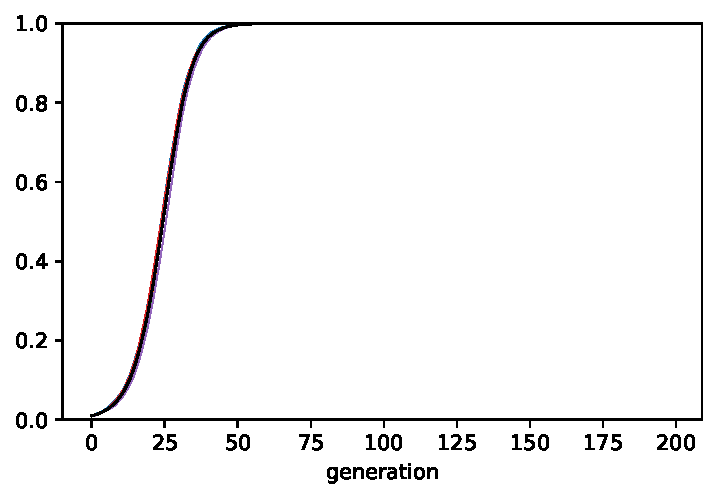
\includegraphics{biased_mutation_files/figure-pdf/cell-7-output-1.pdf}

}

\end{figure}

\part{Modeling biases}

\hypertarget{sec-direct-biased-transmission}{%
\chapter{Biased transmission: direct
bias}\label{sec-direct-biased-transmission}}

\begin{tcolorbox}[enhanced jigsaw, arc=.35mm, colbacktitle=quarto-callout-note-color!10!white, colback=white, breakable, toprule=.15mm, title=\textcolor{quarto-callout-note-color}{\faInfo}\hspace{0.5em}{Note}, left=2mm, bottomtitle=1mm, toptitle=1mm, leftrule=.75mm, opacitybacktitle=0.6, titlerule=0mm, opacityback=0, rightrule=.15mm, bottomrule=.15mm, coltitle=black, colframe=quarto-callout-note-color-frame]

This chapter is based on ``Chapter 3: Biased transmission: direct bias''
in Acerbi et al. (2022).

\end{tcolorbox}

\begin{Shaded}
\begin{Highlighting}[]
\ImportTok{import}\NormalTok{ numpy }\ImportTok{as}\NormalTok{ np}
\NormalTok{rng }\OperatorTok{=}\NormalTok{ np.random.default\_rng()}
\ImportTok{import}\NormalTok{ pandas }\ImportTok{as}\NormalTok{ pd}
\end{Highlighting}
\end{Shaded}

\begin{Shaded}
\begin{Highlighting}[]
\KeywordTok{def}\NormalTok{ plot\_multiple\_runs(data\_model):}
\NormalTok{    groups }\OperatorTok{=}\NormalTok{ data\_model.groupby(}\StringTok{"run"}\NormalTok{)}
    \ControlFlowTok{for}\NormalTok{ \_, g }\KeywordTok{in}\NormalTok{ groups:}
\NormalTok{        g.index }\OperatorTok{=}\NormalTok{ g[}\StringTok{"generation"}\NormalTok{]}
\NormalTok{        g[}\StringTok{"p"}\NormalTok{].plot(lw}\OperatorTok{=}\FloatTok{.5}\NormalTok{, ylim}\OperatorTok{=}\NormalTok{(}\DecValTok{0}\NormalTok{,}\DecValTok{1}\NormalTok{))}

\NormalTok{    data\_model.groupby(}\StringTok{"generation"}\NormalTok{)[}\StringTok{"p"}\NormalTok{].mean().plot(c}\OperatorTok{=}\StringTok{"k"}\NormalTok{, lw}\OperatorTok{=}\StringTok{"1"}\NormalTok{)}
\end{Highlighting}
\end{Shaded}

\begin{Shaded}
\begin{Highlighting}[]
\KeywordTok{def}\NormalTok{ biased\_transmission\_direct(N, s\_a, s\_b, p\_0, t\_max, r\_max):}
    \CommentTok{\# Create the output DataFrame}
\NormalTok{    output }\OperatorTok{=}\NormalTok{ pd.DataFrame(\{}
        \StringTok{"generation"}\NormalTok{ : np.tile(np.arange(t\_max), r\_max),}
        \StringTok{"p"}\NormalTok{ : [ np.nan ] }\OperatorTok{*}\NormalTok{ t\_max }\OperatorTok{*}\NormalTok{ r\_max,}
        \StringTok{"run"}\NormalTok{ : np.repeat(np.arange(r\_max), t\_max)}
\NormalTok{    \})}

    \ControlFlowTok{for}\NormalTok{ r }\KeywordTok{in} \BuiltInTok{range}\NormalTok{(r\_max):}
        \CommentTok{\# Create first generation}
\NormalTok{        population }\OperatorTok{=}\NormalTok{ pd.DataFrame(\{}\StringTok{"trait"}\NormalTok{: rng.choice([}\StringTok{"A"}\NormalTok{, }\StringTok{"B"}\NormalTok{], size}\OperatorTok{=}\NormalTok{N, replace}\OperatorTok{=}\VariableTok{True}\NormalTok{, p}\OperatorTok{=}\NormalTok{[p\_0, }\DecValTok{1} \OperatorTok{{-}}\NormalTok{ p\_0])\})}

        \CommentTok{\# Add first generation\textquotesingle{}s p for run r}
\NormalTok{        output.loc[ r }\OperatorTok{*}\NormalTok{ t\_max, }\StringTok{"p"}\NormalTok{] }\OperatorTok{=}\NormalTok{ population[ population[}\StringTok{"trait"}\NormalTok{] }\OperatorTok{==} \StringTok{"A"}\NormalTok{ ].shape[}\DecValTok{0}\NormalTok{] }\OperatorTok{/}\NormalTok{ N}

        \CommentTok{\# For each generation }
        \ControlFlowTok{for}\NormalTok{ t }\KeywordTok{in} \BuiltInTok{range}\NormalTok{(}\DecValTok{1}\NormalTok{,t\_max):}
            \CommentTok{\# Copy individuals to previous\_population DataFrame}
\NormalTok{            previous\_population }\OperatorTok{=}\NormalTok{ population.copy()}

            \CommentTok{\# For each individual, pick a random individual from the previous generation}
\NormalTok{            demonstrator\_trait }\OperatorTok{=}\NormalTok{ previous\_population[}\StringTok{"trait"}\NormalTok{].sample(N, replace}\OperatorTok{=}\VariableTok{True}\NormalTok{).reset\_index()}
            
            \CommentTok{\# Biased probabilities to copy}
\NormalTok{            copy\_a }\OperatorTok{=}\NormalTok{ rng.choice([}\VariableTok{True}\NormalTok{, }\VariableTok{False}\NormalTok{], size}\OperatorTok{=}\NormalTok{N, replace}\OperatorTok{=}\VariableTok{True}\NormalTok{, p}\OperatorTok{=}\NormalTok{[s\_a, }\DecValTok{1} \OperatorTok{{-}}\NormalTok{ s\_a])}
\NormalTok{            copy\_b }\OperatorTok{=}\NormalTok{ rng.choice([}\VariableTok{True}\NormalTok{, }\VariableTok{False}\NormalTok{], size}\OperatorTok{=}\NormalTok{N, replace}\OperatorTok{=}\VariableTok{True}\NormalTok{, p}\OperatorTok{=}\NormalTok{[s\_b, }\DecValTok{1} \OperatorTok{{-}}\NormalTok{ s\_b])}

            \CommentTok{\# If the demonstrator has trait A and the individual wants to copy A, then copy A}
\NormalTok{            condition }\OperatorTok{=}\NormalTok{ copy\_a }\OperatorTok{\&}\NormalTok{ (demonstrator\_trait[}\StringTok{"trait"}\NormalTok{] }\OperatorTok{==} \StringTok{"A"}\NormalTok{)}
            \ControlFlowTok{if}\NormalTok{ condition.}\BuiltInTok{sum}\NormalTok{() }\OperatorTok{\textgreater{}} \DecValTok{0}\NormalTok{:}
\NormalTok{                population.loc[condition, }\StringTok{"trait"}\NormalTok{] }\OperatorTok{=} \StringTok{"A"}

            \CommentTok{\# If the demonstrator has trait B and the individual wants to copy B, then copy B}
\NormalTok{            condition }\OperatorTok{=}\NormalTok{ copy\_b }\OperatorTok{\&}\NormalTok{ (demonstrator\_trait[}\StringTok{"trait"}\NormalTok{] }\OperatorTok{==} \StringTok{"B"}\NormalTok{)}
            \ControlFlowTok{if}\NormalTok{ condition.}\BuiltInTok{sum}\NormalTok{() }\OperatorTok{\textgreater{}} \DecValTok{0}\NormalTok{:}
\NormalTok{                population.loc[condition, }\StringTok{"trait"}\NormalTok{] }\OperatorTok{=} \StringTok{"B"}

            \CommentTok{\# Get p and put it into output slot for this generation t and run r}
\NormalTok{            output.loc[r }\OperatorTok{*}\NormalTok{ t\_max }\OperatorTok{+}\NormalTok{ t, }\StringTok{"p"}\NormalTok{] }\OperatorTok{=}\NormalTok{ population[ population[}\StringTok{"trait"}\NormalTok{] }\OperatorTok{==} \StringTok{"A"}\NormalTok{ ].shape[}\DecValTok{0}\NormalTok{] }\OperatorTok{/}\NormalTok{ N}

    \ControlFlowTok{return}\NormalTok{ output }
\end{Highlighting}
\end{Shaded}

\begin{Shaded}
\begin{Highlighting}[]
\NormalTok{data\_model }\OperatorTok{=}\NormalTok{ biased\_transmission\_direct(N}\OperatorTok{=}\DecValTok{10\_000}\NormalTok{, s\_a}\OperatorTok{=}\FloatTok{.1}\NormalTok{, s\_b}\OperatorTok{=}\DecValTok{0}\NormalTok{, }
\NormalTok{                                         p\_0}\OperatorTok{=}\FloatTok{.01}\NormalTok{, t\_max}\OperatorTok{=}\DecValTok{200}\NormalTok{, r\_max}\OperatorTok{=}\DecValTok{5}\NormalTok{)}
\NormalTok{plot\_multiple\_runs(data\_model)}
\end{Highlighting}
\end{Shaded}

\begin{figure}[H]

{\centering \includegraphics{chapter05_files/figure-pdf/cell-5-output-1.pdf}

}

\end{figure}

\begin{Shaded}
\begin{Highlighting}[]
\NormalTok{data\_model }\OperatorTok{=}\NormalTok{ biased\_transmission\_direct(N}\OperatorTok{=}\DecValTok{10\_000}\NormalTok{, s\_a}\OperatorTok{=}\FloatTok{.6}\NormalTok{, s\_b}\OperatorTok{=}\FloatTok{.5}\NormalTok{, }
\NormalTok{                                         p\_0}\OperatorTok{=}\FloatTok{.01}\NormalTok{, t\_max}\OperatorTok{=}\DecValTok{150}\NormalTok{, r\_max}\OperatorTok{=}\DecValTok{5}\NormalTok{)}
\NormalTok{plot\_multiple\_runs(data\_model)}
\end{Highlighting}
\end{Shaded}

\begin{figure}[H]

{\centering 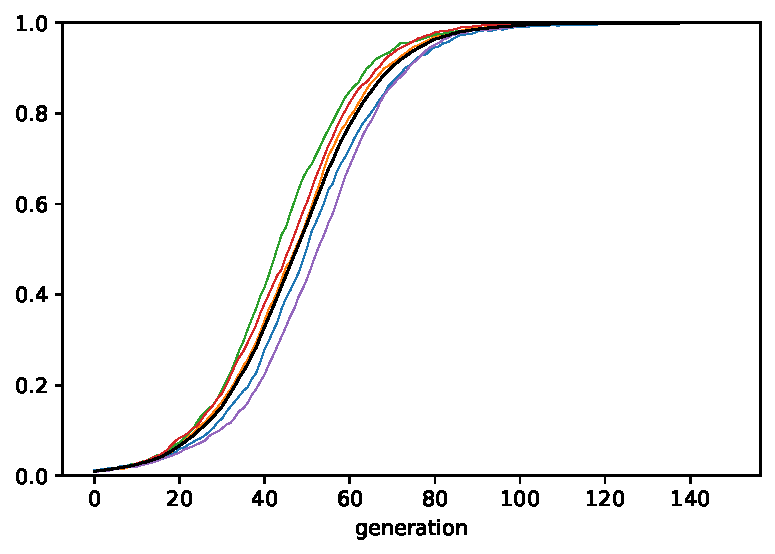
\includegraphics{chapter05_files/figure-pdf/cell-6-output-1.pdf}

}

\end{figure}

\begin{Shaded}
\begin{Highlighting}[]
\NormalTok{data\_model }\OperatorTok{=}\NormalTok{ biased\_transmission\_direct(N}\OperatorTok{=}\DecValTok{10\_000}\NormalTok{, s\_a}\OperatorTok{=}\FloatTok{.2}\NormalTok{, s\_b}\OperatorTok{=}\DecValTok{0}\NormalTok{, }
\NormalTok{                                         p\_0}\OperatorTok{=}\FloatTok{.01}\NormalTok{, t\_max}\OperatorTok{=}\DecValTok{200}\NormalTok{, r\_max}\OperatorTok{=}\DecValTok{5}\NormalTok{)}
\NormalTok{plot\_multiple\_runs(data\_model)}
\end{Highlighting}
\end{Shaded}

\begin{figure}[H]

{\centering 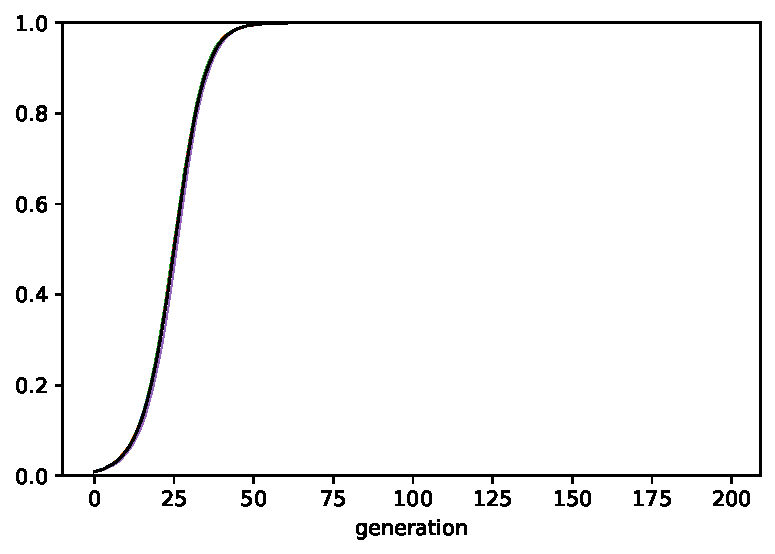
\includegraphics{chapter05_files/figure-pdf/cell-7-output-1.pdf}

}

\end{figure}

\hypertarget{sec-frequency-biased-transmission}{%
\chapter{Biased transmission: frequency-dependent indirect
bias}\label{sec-frequency-biased-transmission}}

\begin{tcolorbox}[enhanced jigsaw, arc=.35mm, colbacktitle=quarto-callout-note-color!10!white, colback=white, breakable, toprule=.15mm, title=\textcolor{quarto-callout-note-color}{\faInfo}\hspace{0.5em}{Note}, left=2mm, bottomtitle=1mm, toptitle=1mm, leftrule=.75mm, opacitybacktitle=0.6, titlerule=0mm, opacityback=0, rightrule=.15mm, bottomrule=.15mm, coltitle=black, colframe=quarto-callout-note-color-frame]

This chapter is based on ``Chapter 4: Biased transmission:
frequency-dependent indirect bias'' in Acerbi et al. (2022).

\end{tcolorbox}

\begin{Shaded}
\begin{Highlighting}[]
\ImportTok{import}\NormalTok{ numpy }\ImportTok{as}\NormalTok{ np }
\NormalTok{rng }\OperatorTok{=}\NormalTok{ np.random.default\_rng()}

\ImportTok{import}\NormalTok{ pandas }\ImportTok{as}\NormalTok{ pd}
\end{Highlighting}
\end{Shaded}

\begin{Shaded}
\begin{Highlighting}[]
\KeywordTok{def}\NormalTok{ plot\_multiple\_runs(data\_model):}
\NormalTok{    groups }\OperatorTok{=}\NormalTok{ data\_model.groupby(}\StringTok{"run"}\NormalTok{)}
    \ControlFlowTok{for}\NormalTok{ \_, g }\KeywordTok{in}\NormalTok{ groups:}
\NormalTok{        g.index }\OperatorTok{=}\NormalTok{ g[}\StringTok{"generation"}\NormalTok{]}
\NormalTok{        g[}\StringTok{"p"}\NormalTok{].plot(lw}\OperatorTok{=}\FloatTok{.5}\NormalTok{, ylim}\OperatorTok{=}\NormalTok{(}\DecValTok{0}\NormalTok{,}\DecValTok{1}\NormalTok{))}

\NormalTok{    data\_model.groupby(}\StringTok{"generation"}\NormalTok{)[}\StringTok{"p"}\NormalTok{].mean().plot(c}\OperatorTok{=}\StringTok{"k"}\NormalTok{, lw}\OperatorTok{=}\StringTok{"1"}\NormalTok{)}
\end{Highlighting}
\end{Shaded}

\begin{Shaded}
\begin{Highlighting}[]
\NormalTok{N }\OperatorTok{=} \DecValTok{100}
\NormalTok{p\_0 }\OperatorTok{=} \FloatTok{.5}
\NormalTok{D }\OperatorTok{=} \FloatTok{1.}
\end{Highlighting}
\end{Shaded}

\begin{Shaded}
\begin{Highlighting}[]
\CommentTok{\# Create first generation}
\NormalTok{population }\OperatorTok{=}\NormalTok{ pd.DataFrame(\{}\StringTok{"trait"}\NormalTok{: rng.choice([}\StringTok{"A"}\NormalTok{, }\StringTok{"B"}\NormalTok{], size}\OperatorTok{=}\NormalTok{N, replace}\OperatorTok{=}\VariableTok{True}\NormalTok{, p}\OperatorTok{=}\NormalTok{[p\_0, }\DecValTok{1}\OperatorTok{{-}}\NormalTok{p\_0])\})}
\end{Highlighting}
\end{Shaded}

\begin{Shaded}
\begin{Highlighting}[]
\CommentTok{\# Create a DataFrame with a set of 3 randomly{-}picked demonstrators for each agent}

\NormalTok{demonstrators }\OperatorTok{=}\NormalTok{ pd.DataFrame(\{}
    \StringTok{"dem1"}\NormalTok{ : population[}\StringTok{"trait"}\NormalTok{].sample(N, replace}\OperatorTok{=}\VariableTok{True}\NormalTok{).values,}
    \StringTok{"dem2"}\NormalTok{ : population[}\StringTok{"trait"}\NormalTok{].sample(N, replace}\OperatorTok{=}\VariableTok{True}\NormalTok{).values,}
    \StringTok{"dem3"}\NormalTok{ : population[}\StringTok{"trait"}\NormalTok{].sample(N, replace}\OperatorTok{=}\VariableTok{True}\NormalTok{).values}
\NormalTok{\})}
\end{Highlighting}
\end{Shaded}

\begin{Shaded}
\begin{Highlighting}[]
\CommentTok{\# Visualize the DataFrame}
\NormalTok{demonstrators.head()}
\end{Highlighting}
\end{Shaded}

\begin{verbatim}
/home/fmoss/.local/lib/python3.10/site-packages/IPython/core/formatters.py:343: FutureWarning: In future versions `DataFrame.to_latex` is expected to utilise the base implementation of `Styler.to_latex` for formatting and rendering. The arguments signature may therefore change. It is recommended instead to use `DataFrame.style.to_latex` which also contains additional functionality.
  return method()
\end{verbatim}

\begin{tabular}{llll}
\toprule
{} & dem1 & dem2 & dem3 \\
\midrule
0 &    A &    A &    A \\
1 &    B &    B &    B \\
2 &    A &    A &    A \\
3 &    B &    A &    A \\
4 &    A &    B &    A \\
\bottomrule
\end{tabular}

\begin{Shaded}
\begin{Highlighting}[]
\CommentTok{\# Get the number of A\textquotesingle{}s in each 3{-}demonstrator combination}
\NormalTok{num\_As }\OperatorTok{=}\NormalTok{ (demonstrators }\OperatorTok{==} \StringTok{"A"}\NormalTok{).}\BuiltInTok{apply}\NormalTok{(}\BuiltInTok{sum}\NormalTok{, axis}\OperatorTok{=}\DecValTok{1}\NormalTok{)}
\NormalTok{num\_As.head()}
\end{Highlighting}
\end{Shaded}

\begin{verbatim}
/home/fmoss/.local/lib/python3.10/site-packages/IPython/core/formatters.py:343: FutureWarning: In future versions `DataFrame.to_latex` is expected to utilise the base implementation of `Styler.to_latex` for formatting and rendering. The arguments signature may therefore change. It is recommended instead to use `DataFrame.style.to_latex` which also contains additional functionality.
  return method()
\end{verbatim}

\begin{tabular}{lr}
\toprule
{} &  0 \\
\midrule
0 &  3 \\
1 &  0 \\
2 &  3 \\
3 &  2 \\
4 &  2 \\
\bottomrule
\end{tabular}

\begin{Shaded}
\begin{Highlighting}[]
\CommentTok{\# For 3{-}demonstrator combinations with all A\textquotesingle{}s, set to A}
\NormalTok{population[ num\_As }\OperatorTok{==} \DecValTok{3}\NormalTok{ ] }\OperatorTok{=} \StringTok{"A"}
\CommentTok{\# For 3{-}demonstrator combinations with all B\textquotesingle{}s, set to B}
\NormalTok{population[ num\_As }\OperatorTok{==} \DecValTok{0}\NormalTok{ ] }\OperatorTok{=} \StringTok{"B"}
\end{Highlighting}
\end{Shaded}

\begin{Shaded}
\begin{Highlighting}[]
\NormalTok{prob\_majority }\OperatorTok{=}\NormalTok{ rng.choice([}\VariableTok{True}\NormalTok{, }\VariableTok{False}\NormalTok{], p}\OperatorTok{=}\NormalTok{[(}\DecValTok{2}\OperatorTok{/}\DecValTok{3} \OperatorTok{+}\NormalTok{ D}\OperatorTok{/}\DecValTok{3}\NormalTok{), }\DecValTok{1}\OperatorTok{{-}}\NormalTok{(}\DecValTok{2}\OperatorTok{/}\DecValTok{3} \OperatorTok{+}\NormalTok{ D}\OperatorTok{/}\DecValTok{3}\NormalTok{)], size}\OperatorTok{=}\NormalTok{N, replace}\OperatorTok{=}\VariableTok{True}\NormalTok{)}
\NormalTok{prob\_minority }\OperatorTok{=}\NormalTok{ rng.choice([}\VariableTok{True}\NormalTok{, }\VariableTok{False}\NormalTok{], p}\OperatorTok{=}\NormalTok{[(}\DecValTok{1}\OperatorTok{/}\DecValTok{3} \OperatorTok{+}\NormalTok{ D}\OperatorTok{/}\DecValTok{3}\NormalTok{), }\DecValTok{1}\OperatorTok{{-}}\NormalTok{(}\DecValTok{1}\OperatorTok{/}\DecValTok{3} \OperatorTok{+}\NormalTok{ D}\OperatorTok{/}\DecValTok{3}\NormalTok{)], size}\OperatorTok{=}\NormalTok{N, replace}\OperatorTok{=}\VariableTok{True}\NormalTok{)}
\end{Highlighting}
\end{Shaded}

\begin{Shaded}
\begin{Highlighting}[]
\CommentTok{\# 3{-}demonstrator combinations with two As and one B}
\NormalTok{condition }\OperatorTok{=}\NormalTok{ prob\_majority }\OperatorTok{\&}\NormalTok{ (num\_As }\OperatorTok{==} \DecValTok{2}\NormalTok{)}
\ControlFlowTok{if}\NormalTok{ condition.}\BuiltInTok{sum}\NormalTok{() }\OperatorTok{\textgreater{}} \DecValTok{0}\NormalTok{:}
\NormalTok{    population.loc[condition, }\StringTok{"trait"}\NormalTok{] }\OperatorTok{=} \StringTok{"A"}
\NormalTok{condition }\OperatorTok{=} \OperatorTok{\textasciitilde{}}\NormalTok{prob\_majority }\OperatorTok{\&}\NormalTok{ (num\_As }\OperatorTok{==} \DecValTok{2}\NormalTok{)}
\ControlFlowTok{if}\NormalTok{ condition.}\BuiltInTok{sum}\NormalTok{() }\OperatorTok{\textgreater{}} \DecValTok{0}\NormalTok{:}
\NormalTok{    population.loc[condition, }\StringTok{"trait"}\NormalTok{] }\OperatorTok{=} \StringTok{"B"}

\CommentTok{\# 3{-}demonstrator combinations with two B\textquotesingle{}s and one A}
\NormalTok{condition }\OperatorTok{=} \OperatorTok{\textasciitilde{}}\NormalTok{prob\_minority }\OperatorTok{\&}\NormalTok{ (num\_As }\OperatorTok{==} \DecValTok{1}\NormalTok{)}
\ControlFlowTok{if}\NormalTok{ condition.}\BuiltInTok{sum}\NormalTok{() }\OperatorTok{\textgreater{}} \DecValTok{0}\NormalTok{:}
\NormalTok{    population.loc[condition, }\StringTok{"trait"}\NormalTok{] }\OperatorTok{=} \StringTok{"A"}
\NormalTok{condition }\OperatorTok{=}\NormalTok{ prob\_minority }\OperatorTok{\&}\NormalTok{ (num\_As }\OperatorTok{==} \DecValTok{1}\NormalTok{)}
\ControlFlowTok{if}\NormalTok{ condition.}\BuiltInTok{sum}\NormalTok{() }\OperatorTok{\textgreater{}} \DecValTok{0}\NormalTok{:}
\NormalTok{    population.loc[condition, }\StringTok{"trait"}\NormalTok{] }\OperatorTok{=} \StringTok{"B"}
\end{Highlighting}
\end{Shaded}

\begin{Shaded}
\begin{Highlighting}[]
\NormalTok{demonstrators[}\StringTok{"new\_trait"}\NormalTok{] }\OperatorTok{=}\NormalTok{ population[}\StringTok{"trait"}\NormalTok{]}
\NormalTok{demonstrators.head()}
\end{Highlighting}
\end{Shaded}

\begin{verbatim}
/home/fmoss/.local/lib/python3.10/site-packages/IPython/core/formatters.py:343: FutureWarning: In future versions `DataFrame.to_latex` is expected to utilise the base implementation of `Styler.to_latex` for formatting and rendering. The arguments signature may therefore change. It is recommended instead to use `DataFrame.style.to_latex` which also contains additional functionality.
  return method()
\end{verbatim}

\begin{tabular}{lllll}
\toprule
{} & dem1 & dem2 & dem3 & new\_trait \\
\midrule
0 &    A &    A &    A &         A \\
1 &    B &    B &    B &         B \\
2 &    A &    A &    A &         A \\
3 &    B &    A &    A &         A \\
4 &    A &    B &    A &         A \\
\bottomrule
\end{tabular}

\begin{Shaded}
\begin{Highlighting}[]
\KeywordTok{def}\NormalTok{ conformist\_transmission(N, p\_0, D, t\_max, r\_max):}
    \CommentTok{\# Create the output DataFrame}
\NormalTok{    output }\OperatorTok{=}\NormalTok{ pd.DataFrame(\{}
        \StringTok{"generation"}\NormalTok{ : np.tile(np.arange(t\_max), r\_max),}
        \StringTok{"p"}\NormalTok{ : [ np.nan ] }\OperatorTok{*}\NormalTok{ t\_max }\OperatorTok{*}\NormalTok{ r\_max,}
        \StringTok{"run"}\NormalTok{ : np.repeat(np.arange(r\_max), t\_max)}
\NormalTok{    \})}

    \ControlFlowTok{for}\NormalTok{ r }\KeywordTok{in} \BuiltInTok{range}\NormalTok{(r\_max):}
        \CommentTok{\# Create first generation}
\NormalTok{        population }\OperatorTok{=}\NormalTok{ pd.DataFrame(\{}\StringTok{"trait"}\NormalTok{: rng.choice([}\StringTok{"A"}\NormalTok{, }\StringTok{"B"}\NormalTok{], size}\OperatorTok{=}\NormalTok{N, replace}\OperatorTok{=}\VariableTok{True}\NormalTok{, p}\OperatorTok{=}\NormalTok{[p\_0, }\DecValTok{1} \OperatorTok{{-}}\NormalTok{ p\_0])\})}

        \CommentTok{\# Add first generation\textquotesingle{}s p for run r}
\NormalTok{        output.loc[ r }\OperatorTok{*}\NormalTok{ t\_max, }\StringTok{"p"}\NormalTok{] }\OperatorTok{=}\NormalTok{ population[ population[}\StringTok{"trait"}\NormalTok{] }\OperatorTok{==} \StringTok{"A"}\NormalTok{ ].shape[}\DecValTok{0}\NormalTok{] }\OperatorTok{/}\NormalTok{ N}

        \CommentTok{\# For each generation }
        \ControlFlowTok{for}\NormalTok{ t }\KeywordTok{in} \BuiltInTok{range}\NormalTok{(}\DecValTok{1}\NormalTok{,t\_max):}
\NormalTok{            demonstrators }\OperatorTok{=}\NormalTok{ pd.DataFrame(\{}
                \StringTok{"dem1"}\NormalTok{ : population[}\StringTok{"trait"}\NormalTok{].sample(N, replace}\OperatorTok{=}\VariableTok{True}\NormalTok{).values,}
                \StringTok{"dem2"}\NormalTok{ : population[}\StringTok{"trait"}\NormalTok{].sample(N, replace}\OperatorTok{=}\VariableTok{True}\NormalTok{).values,}
                \StringTok{"dem3"}\NormalTok{ : population[}\StringTok{"trait"}\NormalTok{].sample(N, replace}\OperatorTok{=}\VariableTok{True}\NormalTok{).values}
\NormalTok{            \})}

            \CommentTok{\# Get the number of A\textquotesingle{}s in each 3{-}demonstrator combination}
\NormalTok{            num\_As }\OperatorTok{=}\NormalTok{ (demonstrators }\OperatorTok{==} \StringTok{"A"}\NormalTok{).}\BuiltInTok{apply}\NormalTok{(}\BuiltInTok{sum}\NormalTok{, axis}\OperatorTok{=}\DecValTok{1}\NormalTok{)}

            \CommentTok{\# For 3{-}demonstrator combinations with all A\textquotesingle{}s, set to A}
\NormalTok{            population[ num\_As }\OperatorTok{==} \DecValTok{3}\NormalTok{ ] }\OperatorTok{=} \StringTok{"A"}
            \CommentTok{\# For 3{-}demonstrator combinations with all A\textquotesingle{}s, set to A}
\NormalTok{            population[ num\_As }\OperatorTok{==} \DecValTok{3}\NormalTok{ ] }\OperatorTok{=} \StringTok{"A"}
            \CommentTok{\# For 3{-}demonstrator combinations with all B\textquotesingle{}s, set to B}
\NormalTok{            population[ num\_As }\OperatorTok{==} \DecValTok{0}\NormalTok{ ] }\OperatorTok{=} \StringTok{"B"}

\NormalTok{            prob\_majority }\OperatorTok{=}\NormalTok{ rng.choice([}\VariableTok{True}\NormalTok{, }\VariableTok{False}\NormalTok{], p}\OperatorTok{=}\NormalTok{[(}\DecValTok{2}\OperatorTok{/}\DecValTok{3} \OperatorTok{+}\NormalTok{ D}\OperatorTok{/}\DecValTok{3}\NormalTok{), }\DecValTok{1}\OperatorTok{{-}}\NormalTok{(}\DecValTok{2}\OperatorTok{/}\DecValTok{3} \OperatorTok{+}\NormalTok{ D}\OperatorTok{/}\DecValTok{3}\NormalTok{)], size}\OperatorTok{=}\NormalTok{N, replace}\OperatorTok{=}\VariableTok{True}\NormalTok{)}
\NormalTok{            prob\_minority }\OperatorTok{=}\NormalTok{ rng.choice([}\VariableTok{True}\NormalTok{, }\VariableTok{False}\NormalTok{], p}\OperatorTok{=}\NormalTok{[(}\DecValTok{1}\OperatorTok{/}\DecValTok{3} \OperatorTok{+}\NormalTok{ D}\OperatorTok{/}\DecValTok{3}\NormalTok{), }\DecValTok{1}\OperatorTok{{-}}\NormalTok{(}\DecValTok{1}\OperatorTok{/}\DecValTok{3} \OperatorTok{+}\NormalTok{ D}\OperatorTok{/}\DecValTok{3}\NormalTok{)], size}\OperatorTok{=}\NormalTok{N, replace}\OperatorTok{=}\VariableTok{True}\NormalTok{)}

            \CommentTok{\# 3{-}demonstrator combinations with two As and one B}
\NormalTok{            condition }\OperatorTok{=}\NormalTok{ prob\_majority }\OperatorTok{\&}\NormalTok{ (num\_As }\OperatorTok{==} \DecValTok{2}\NormalTok{)}
            \ControlFlowTok{if}\NormalTok{ condition.}\BuiltInTok{sum}\NormalTok{() }\OperatorTok{\textgreater{}} \DecValTok{0}\NormalTok{:}
\NormalTok{                population.loc[condition, }\StringTok{"trait"}\NormalTok{] }\OperatorTok{=} \StringTok{"A"}
\NormalTok{            condition }\OperatorTok{=} \OperatorTok{\textasciitilde{}}\NormalTok{prob\_majority }\OperatorTok{\&}\NormalTok{ (num\_As }\OperatorTok{==} \DecValTok{2}\NormalTok{)}
            \ControlFlowTok{if}\NormalTok{ condition.}\BuiltInTok{sum}\NormalTok{() }\OperatorTok{\textgreater{}} \DecValTok{0}\NormalTok{:}
\NormalTok{                population.loc[condition, }\StringTok{"trait"}\NormalTok{] }\OperatorTok{=} \StringTok{"B"}

            \CommentTok{\# 3{-}demonstrator combinations with two B\textquotesingle{}s and one A}
\NormalTok{            condition }\OperatorTok{=}\NormalTok{ prob\_minority }\OperatorTok{\&}\NormalTok{ (num\_As }\OperatorTok{==} \DecValTok{1}\NormalTok{)}
            \ControlFlowTok{if}\NormalTok{ condition.}\BuiltInTok{sum}\NormalTok{() }\OperatorTok{\textgreater{}} \DecValTok{0}\NormalTok{:}
\NormalTok{                population.loc[condition, }\StringTok{"trait"}\NormalTok{] }\OperatorTok{=} \StringTok{"A"}
\NormalTok{            condition }\OperatorTok{=} \OperatorTok{\textasciitilde{}}\NormalTok{prob\_minority }\OperatorTok{\&}\NormalTok{ (num\_As }\OperatorTok{==} \DecValTok{1}\NormalTok{)}
            \ControlFlowTok{if}\NormalTok{ condition.}\BuiltInTok{sum}\NormalTok{() }\OperatorTok{\textgreater{}} \DecValTok{0}\NormalTok{:}
\NormalTok{                population.loc[condition, }\StringTok{"trait"}\NormalTok{] }\OperatorTok{=} \StringTok{"B"}
            
            \CommentTok{\# Get p and put it into output slot for this generation t and run r}
\NormalTok{            output.loc[r }\OperatorTok{*}\NormalTok{ t\_max }\OperatorTok{+}\NormalTok{ t, }\StringTok{"p"}\NormalTok{] }\OperatorTok{=}\NormalTok{ population[ population[}\StringTok{"trait"}\NormalTok{] }\OperatorTok{==} \StringTok{"A"}\NormalTok{ ].shape[}\DecValTok{0}\NormalTok{] }\OperatorTok{/}\NormalTok{ N}

    \ControlFlowTok{return}\NormalTok{ output}
\end{Highlighting}
\end{Shaded}

\begin{Shaded}
\begin{Highlighting}[]
\NormalTok{data\_model }\OperatorTok{=}\NormalTok{ conformist\_transmission(N}\OperatorTok{=}\DecValTok{1\_000}\NormalTok{, p\_0 }\OperatorTok{=} \FloatTok{0.5}\NormalTok{, D }\OperatorTok{=} \DecValTok{1}\NormalTok{, t\_max }\OperatorTok{=} \DecValTok{50}\NormalTok{, r\_max }\OperatorTok{=} \DecValTok{10}\NormalTok{)}
\NormalTok{plot\_multiple\_runs(data\_model)}
\end{Highlighting}
\end{Shaded}

\begin{figure}[H]

{\centering 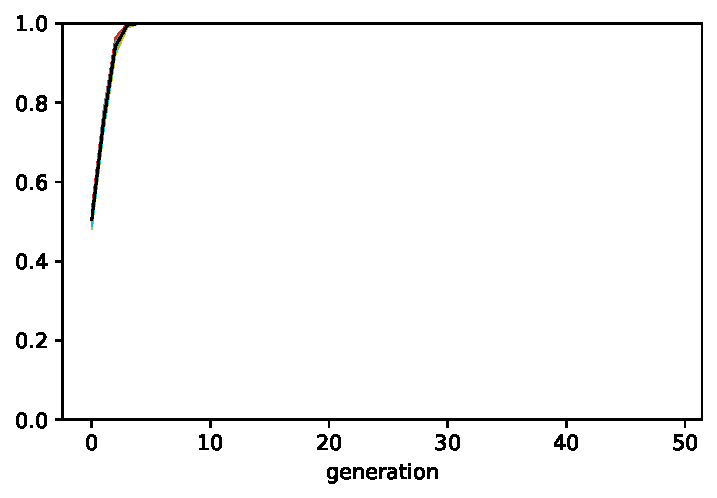
\includegraphics{chapter06_files/figure-pdf/cell-14-output-1.pdf}

}

\end{figure}

\hypertarget{sec-demonstrator-biased-transmission}{%
\chapter{Biased transmission: influencer-based indirect
bias}\label{sec-demonstrator-biased-transmission}}

\begin{tcolorbox}[enhanced jigsaw, arc=.35mm, colbacktitle=quarto-callout-note-color!10!white, colback=white, breakable, toprule=.15mm, title=\textcolor{quarto-callout-note-color}{\faInfo}\hspace{0.5em}{Note}, left=2mm, bottomtitle=1mm, toptitle=1mm, leftrule=.75mm, opacitybacktitle=0.6, titlerule=0mm, opacityback=0, rightrule=.15mm, bottomrule=.15mm, coltitle=black, colframe=quarto-callout-note-color-frame]

This chapter is based on ``Chapter 5: Biased transmission:
demonstrator-based indirect bias'' in Acerbi et al. (2022).

\end{tcolorbox}

Instead of calling them demonstrators, we will call them influencers.

\begin{figure}

{\centering 
\includegraphics{img/influencer.png}

}

\caption{An influencer on a popular video platform.}

\end{figure}

\begin{Shaded}
\begin{Highlighting}[]
\ImportTok{import}\NormalTok{ numpy }\ImportTok{as}\NormalTok{ np }
\NormalTok{rng }\OperatorTok{=}\NormalTok{ np.random.default\_rng()}

\ImportTok{import}\NormalTok{ pandas }\ImportTok{as}\NormalTok{ pd}
\end{Highlighting}
\end{Shaded}

\begin{Shaded}
\begin{Highlighting}[]
\KeywordTok{def}\NormalTok{ plot\_multiple\_runs(data\_model):}
\NormalTok{    groups }\OperatorTok{=}\NormalTok{ data\_model.groupby(}\StringTok{"run"}\NormalTok{)}
    \ControlFlowTok{for}\NormalTok{ \_, g }\KeywordTok{in}\NormalTok{ groups:}
\NormalTok{        g.index }\OperatorTok{=}\NormalTok{ g[}\StringTok{"generation"}\NormalTok{]}
\NormalTok{        g[}\StringTok{"p"}\NormalTok{].plot(lw}\OperatorTok{=}\FloatTok{.5}\NormalTok{, ylim}\OperatorTok{=}\NormalTok{(}\DecValTok{0}\NormalTok{,}\DecValTok{1}\NormalTok{))}

\NormalTok{    data\_model.groupby(}\StringTok{"generation"}\NormalTok{)[}\StringTok{"p"}\NormalTok{].mean().plot(c}\OperatorTok{=}\StringTok{"k"}\NormalTok{, lw}\OperatorTok{=}\StringTok{"1"}\NormalTok{)}
\end{Highlighting}
\end{Shaded}

\begin{Shaded}
\begin{Highlighting}[]
\NormalTok{N }\OperatorTok{=} \DecValTok{100}
\NormalTok{p\_0 }\OperatorTok{=} \FloatTok{0.5}
\NormalTok{p\_s }\OperatorTok{=} \FloatTok{0.05}
\end{Highlighting}
\end{Shaded}

\begin{Shaded}
\begin{Highlighting}[]
\NormalTok{population }\OperatorTok{=}\NormalTok{ pd.DataFrame(\{}
    \StringTok{"trait"}\NormalTok{: rng.choice([}\StringTok{"A"}\NormalTok{, }\StringTok{"B"}\NormalTok{], size}\OperatorTok{=}\NormalTok{N, replace}\OperatorTok{=}\VariableTok{True}\NormalTok{, p}\OperatorTok{=}\NormalTok{[p\_0, }\DecValTok{1}\OperatorTok{{-}}\NormalTok{p\_0]),}
    \StringTok{"status"}\NormalTok{: rng.choice([}\StringTok{"high"}\NormalTok{, }\StringTok{"low"}\NormalTok{], size}\OperatorTok{=}\NormalTok{N, replace}\OperatorTok{=}\VariableTok{True}\NormalTok{, p}\OperatorTok{=}\NormalTok{[p\_s, }\DecValTok{1}\OperatorTok{{-}}\NormalTok{p\_s])}
\NormalTok{\})}
\end{Highlighting}
\end{Shaded}

\begin{Shaded}
\begin{Highlighting}[]
\NormalTok{population.head()}
\end{Highlighting}
\end{Shaded}

\begin{tabular}{lll}
\toprule
{} & trait & status \\
\midrule
0 &     A &    low \\
1 &     A &    low \\
2 &     A &    low \\
3 &     A &    low \\
4 &     B &    low \\
\bottomrule
\end{tabular}

\begin{Shaded}
\begin{Highlighting}[]
\NormalTok{p\_low }\OperatorTok{=} \FloatTok{0.01}
\NormalTok{p\_influencer }\OperatorTok{=}\NormalTok{ np.ones(N)}
\NormalTok{p\_influencer[ population[}\StringTok{"status"}\NormalTok{] }\OperatorTok{==} \StringTok{"low"}\NormalTok{ ] }\OperatorTok{=}\NormalTok{ p\_low}
\end{Highlighting}
\end{Shaded}

\begin{Shaded}
\begin{Highlighting}[]
\ControlFlowTok{if} \BuiltInTok{sum}\NormalTok{(p\_influencer) }\OperatorTok{\textgreater{}} \DecValTok{0}\NormalTok{:}
\NormalTok{    ps }\OperatorTok{=}\NormalTok{ p\_influencer }\OperatorTok{/}\NormalTok{ p\_influencer.}\BuiltInTok{sum}\NormalTok{()}
\NormalTok{    influencer\_index }\OperatorTok{=}\NormalTok{ rng.choice(np.arange(N), size}\OperatorTok{=}\NormalTok{N, p}\OperatorTok{=}\NormalTok{ps, replace}\OperatorTok{=}\VariableTok{True}\NormalTok{)}
\NormalTok{    population[}\StringTok{"trait"}\NormalTok{] }\OperatorTok{=}\NormalTok{ population.loc[influencer\_index, }\StringTok{"trait"}\NormalTok{].values}
\end{Highlighting}
\end{Shaded}

\begin{Shaded}
\begin{Highlighting}[]
\KeywordTok{def}\NormalTok{ biased\_transmission\_influencer(N, p\_0, p\_s, p\_low, t\_max, r\_max):}
    \CommentTok{\# Create the output DataFrame}
\NormalTok{    output }\OperatorTok{=}\NormalTok{ pd.DataFrame(\{}
        \StringTok{"generation"}\NormalTok{ : np.tile(np.arange(t\_max), r\_max),}
        \StringTok{"p"}\NormalTok{ : [ np.nan ] }\OperatorTok{*}\NormalTok{ t\_max }\OperatorTok{*}\NormalTok{ r\_max,}
        \StringTok{"run"}\NormalTok{ : np.repeat(np.arange(r\_max), t\_max)}
\NormalTok{    \})}
    
    \ControlFlowTok{for}\NormalTok{ r }\KeywordTok{in} \BuiltInTok{range}\NormalTok{(r\_max):}
            \CommentTok{\# Create first generation}
\NormalTok{            population }\OperatorTok{=}\NormalTok{ pd.DataFrame(\{}
                \StringTok{"trait"}\NormalTok{: rng.choice([}\StringTok{"A"}\NormalTok{, }\StringTok{"B"}\NormalTok{], size}\OperatorTok{=}\NormalTok{N, replace}\OperatorTok{=}\VariableTok{True}\NormalTok{, p}\OperatorTok{=}\NormalTok{[p\_0, }\DecValTok{1}\OperatorTok{{-}}\NormalTok{p\_0]),}
                \StringTok{"status"}\NormalTok{: rng.choice([}\StringTok{"high"}\NormalTok{, }\StringTok{"low"}\NormalTok{], size}\OperatorTok{=}\NormalTok{N, replace}\OperatorTok{=}\VariableTok{True}\NormalTok{, p}\OperatorTok{=}\NormalTok{[p\_s, }\DecValTok{1}\OperatorTok{{-}}\NormalTok{p\_s])}
\NormalTok{            \})}
            
            \CommentTok{\# Assign copying probabilities based on individuals\textquotesingle{} status}
\NormalTok{            p\_influencer }\OperatorTok{=}\NormalTok{ np.ones(N)}
\NormalTok{            p\_influencer[population[}\StringTok{"status"}\NormalTok{] }\OperatorTok{==} \StringTok{"low"}\NormalTok{] }\OperatorTok{=}\NormalTok{ p\_low}
            
            \CommentTok{\# Add first generation\textquotesingle{}s p for run r}
\NormalTok{            output.loc[ r }\OperatorTok{*}\NormalTok{ t\_max, }\StringTok{"p"}\NormalTok{] }\OperatorTok{=}\NormalTok{ population[ population[}\StringTok{"trait"}\NormalTok{] }\OperatorTok{==} \StringTok{"A"}\NormalTok{ ].shape[}\DecValTok{0}\NormalTok{] }\OperatorTok{/}\NormalTok{ N}
            
            \ControlFlowTok{for}\NormalTok{ t }\KeywordTok{in} \BuiltInTok{range}\NormalTok{(}\DecValTok{1}\NormalTok{, t\_max):}
                \CommentTok{\# Copy individuals to previous\_population DataFrame}
\NormalTok{                previous\_population }\OperatorTok{=}\NormalTok{ population.copy()}
                
                \CommentTok{\# Copy traits based on status}
                \ControlFlowTok{if} \BuiltInTok{sum}\NormalTok{(p\_influencer) }\OperatorTok{\textgreater{}} \DecValTok{0}\NormalTok{:}
\NormalTok{                    ps }\OperatorTok{=}\NormalTok{ p\_influencer }\OperatorTok{/}\NormalTok{ p\_influencer.}\BuiltInTok{sum}\NormalTok{()}
\NormalTok{                    influencer\_index }\OperatorTok{=}\NormalTok{ rng.choice(np.arange(N), size}\OperatorTok{=}\NormalTok{N, p}\OperatorTok{=}\NormalTok{ps, replace}\OperatorTok{=}\VariableTok{True}\NormalTok{)}
\NormalTok{                    population[}\StringTok{"trait"}\NormalTok{] }\OperatorTok{=}\NormalTok{ population.loc[influencer\_index, }\StringTok{"trait"}\NormalTok{].values}
                
                \CommentTok{\# Get p and put it into output slot for this generation t and run r}
\NormalTok{                output.loc[r }\OperatorTok{*}\NormalTok{ t\_max }\OperatorTok{+}\NormalTok{ t, }\StringTok{"p"}\NormalTok{] }\OperatorTok{=}\NormalTok{ population[ population[}\StringTok{"trait"}\NormalTok{] }\OperatorTok{==} \StringTok{"A"}\NormalTok{ ].shape[}\DecValTok{0}\NormalTok{] }\OperatorTok{/}\NormalTok{ N}
                
    \ControlFlowTok{return}\NormalTok{ output}
\end{Highlighting}
\end{Shaded}

\begin{Shaded}
\begin{Highlighting}[]
\NormalTok{data\_model }\OperatorTok{=}\NormalTok{ biased\_transmission\_influencer(N}\OperatorTok{=}\DecValTok{100}\NormalTok{, p\_s}\OperatorTok{=}\FloatTok{0.05}\NormalTok{, p\_low}\OperatorTok{=}\FloatTok{0.0001}\NormalTok{, p\_0}\OperatorTok{=}\FloatTok{0.5}\NormalTok{, t\_max}\OperatorTok{=}\DecValTok{50}\NormalTok{, r\_max}\OperatorTok{=}\DecValTok{10}\NormalTok{)}
\end{Highlighting}
\end{Shaded}

\begin{Shaded}
\begin{Highlighting}[]
\NormalTok{plot\_multiple\_runs(data\_model)}
\end{Highlighting}
\end{Shaded}

\begin{figure}[H]

{\centering 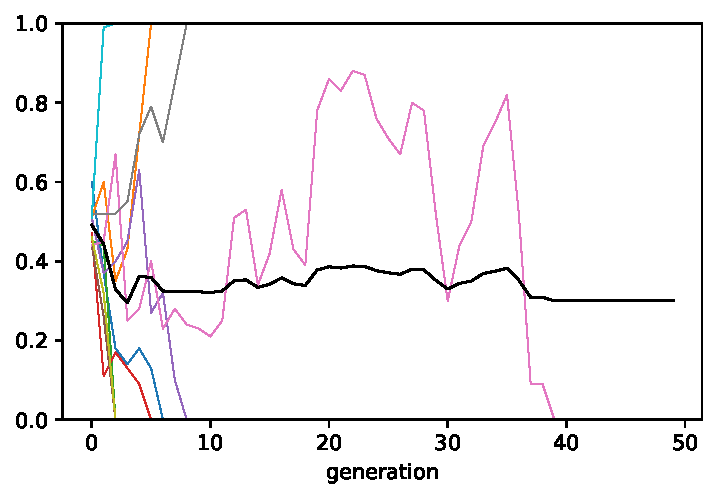
\includegraphics{chapter07_files/figure-pdf/cell-11-output-1.pdf}

}

\end{figure}

\begin{Shaded}
\begin{Highlighting}[]
\NormalTok{data\_model }\OperatorTok{=}\NormalTok{ biased\_transmission\_influencer(N}\OperatorTok{=}\DecValTok{10\_000}\NormalTok{, p\_s}\OperatorTok{=}\FloatTok{0.005}\NormalTok{, p\_low}\OperatorTok{=}\FloatTok{0.0001}\NormalTok{, p\_0}\OperatorTok{=}\FloatTok{0.5}\NormalTok{, t\_max}\OperatorTok{=}\DecValTok{200}\NormalTok{, r\_max}\OperatorTok{=}\DecValTok{10}\NormalTok{)}
\NormalTok{plot\_multiple\_runs(data\_model)}
\end{Highlighting}
\end{Shaded}

\begin{figure}[H]

{\centering 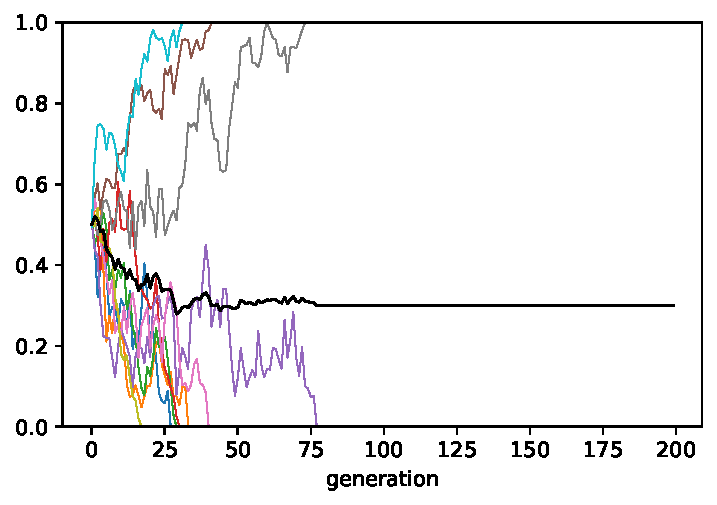
\includegraphics{chapter07_files/figure-pdf/cell-12-output-1.pdf}

}

\end{figure}

\begin{Shaded}
\begin{Highlighting}[]
\KeywordTok{def}\NormalTok{ biased\_transmission\_influencer\_2(N, p\_0, p\_s, p\_low, t\_max, r\_max):}
    \CommentTok{\# Create the output DataFrame}
\NormalTok{    output }\OperatorTok{=}\NormalTok{ pd.DataFrame(\{}
        \StringTok{"generation"}\NormalTok{ : np.tile(np.arange(t\_max), r\_max),}
        \StringTok{"p"}\NormalTok{ : [ np.nan ] }\OperatorTok{*}\NormalTok{ t\_max }\OperatorTok{*}\NormalTok{ r\_max,}
        \StringTok{"run"}\NormalTok{ : np.repeat(np.arange(r\_max), t\_max)}
\NormalTok{    \})}
    
\NormalTok{    ... }\CommentTok{\# }\AlertTok{TODO}
    
    \ControlFlowTok{return}\NormalTok{ output}
\end{Highlighting}
\end{Shaded}

\begin{Shaded}
\begin{Highlighting}[]
\NormalTok{data\_model }\OperatorTok{=}\NormalTok{ biased\_transmission\_influencer\_2(N}\OperatorTok{=}\DecValTok{100}\NormalTok{, p\_s}\OperatorTok{=}\FloatTok{0.1}\NormalTok{, p\_low}\OperatorTok{=}\FloatTok{0.0001}\NormalTok{, p\_0}\OperatorTok{=}\FloatTok{0.5}\NormalTok{, t\_max}\OperatorTok{=}\DecValTok{50}\NormalTok{, r\_max}\OperatorTok{=}\DecValTok{50}\NormalTok{)}
\end{Highlighting}
\end{Shaded}

\hypertarget{sec-vertical-horizontal}{%
\chapter{Vertical and horizontal cultural
transmission}\label{sec-vertical-horizontal}}

\begin{Shaded}
\begin{Highlighting}[]
\ImportTok{import}\NormalTok{ numpy }\ImportTok{as}\NormalTok{ np }
\NormalTok{rng }\OperatorTok{=}\NormalTok{ np.random.default\_rng()}

\ImportTok{import}\NormalTok{ pandas }\ImportTok{as}\NormalTok{ pd}
\ImportTok{from}\NormalTok{ tqdm }\ImportTok{import}\NormalTok{ tqdm}
\end{Highlighting}
\end{Shaded}

\begin{Shaded}
\begin{Highlighting}[]
\KeywordTok{def}\NormalTok{ plot\_multiple\_runs(data\_model):}
\NormalTok{    groups }\OperatorTok{=}\NormalTok{ data\_model.groupby(}\StringTok{"run"}\NormalTok{)}
    \ControlFlowTok{for}\NormalTok{ \_, g }\KeywordTok{in}\NormalTok{ groups:}
\NormalTok{        g.index }\OperatorTok{=}\NormalTok{ g[}\StringTok{"generation"}\NormalTok{]}
\NormalTok{        g[}\StringTok{"p"}\NormalTok{].plot(lw}\OperatorTok{=}\FloatTok{.5}\NormalTok{, ylim}\OperatorTok{=}\NormalTok{(}\DecValTok{0}\NormalTok{,}\DecValTok{1}\NormalTok{))}

\NormalTok{    data\_model.groupby(}\StringTok{"generation"}\NormalTok{)[}\StringTok{"p"}\NormalTok{].mean().plot(c}\OperatorTok{=}\StringTok{"k"}\NormalTok{, lw}\OperatorTok{=}\StringTok{"1"}\NormalTok{)}
\end{Highlighting}
\end{Shaded}

\begin{Shaded}
\begin{Highlighting}[]
\KeywordTok{def}\NormalTok{ vertical\_transmission(N, p\_0, b, t\_max, r\_max):}
    \CommentTok{\# Create the output DataFrame}
\NormalTok{    output }\OperatorTok{=}\NormalTok{ pd.DataFrame(\{}
        \StringTok{"generation"}\NormalTok{ : np.tile(np.arange(t\_max), r\_max),}
        \StringTok{"p"}\NormalTok{ : [ np.nan ] }\OperatorTok{*}\NormalTok{ t\_max }\OperatorTok{*}\NormalTok{ r\_max,}
        \StringTok{"run"}\NormalTok{ : np.repeat(np.arange(r\_max), t\_max)}
\NormalTok{    \})}

    \ControlFlowTok{for}\NormalTok{ r }\KeywordTok{in} \BuiltInTok{range}\NormalTok{(r\_max): }
        \CommentTok{\# Create first generation}
\NormalTok{        population }\OperatorTok{=}\NormalTok{ pd.DataFrame(\{}\StringTok{"trait"}\NormalTok{: rng.choice([}\StringTok{"A"}\NormalTok{, }\StringTok{"B"}\NormalTok{], size}\OperatorTok{=}\NormalTok{N, replace}\OperatorTok{=}\VariableTok{True}\NormalTok{, p}\OperatorTok{=}\NormalTok{[p\_0, }\DecValTok{1} \OperatorTok{{-}}\NormalTok{ p\_0])\})}

        \CommentTok{\# Add first generation\textquotesingle{}s p for run r}
\NormalTok{        output.loc[ r }\OperatorTok{*}\NormalTok{ t\_max, }\StringTok{"p"}\NormalTok{] }\OperatorTok{=}\NormalTok{ population[ population[}\StringTok{"trait"}\NormalTok{] }\OperatorTok{==} \StringTok{"A"}\NormalTok{ ].shape[}\DecValTok{0}\NormalTok{] }\OperatorTok{/}\NormalTok{ N}

        \CommentTok{\# \# For each generation }
        \ControlFlowTok{for}\NormalTok{ t }\KeywordTok{in} \BuiltInTok{range}\NormalTok{(}\DecValTok{1}\NormalTok{, t\_max): }
            \CommentTok{\# Copy individuals to previous\_population DataFrame}
\NormalTok{            previous\_population }\OperatorTok{=}\NormalTok{ population.copy()}

            \CommentTok{\# randomly pick mothers and fathers}
\NormalTok{            mother }\OperatorTok{=}\NormalTok{ previous\_population[}\StringTok{"trait"}\NormalTok{].sample(N, replace}\OperatorTok{=}\VariableTok{True}\NormalTok{).reset\_index(drop}\OperatorTok{=}\VariableTok{True}\NormalTok{)}
\NormalTok{            father }\OperatorTok{=}\NormalTok{ previous\_population[}\StringTok{"trait"}\NormalTok{].sample(N, replace}\OperatorTok{=}\VariableTok{True}\NormalTok{).reset\_index(drop}\OperatorTok{=}\VariableTok{True}\NormalTok{)}

            \CommentTok{\# prepare next generation}
\NormalTok{            population }\OperatorTok{=}\NormalTok{ pd.DataFrame(\{}\StringTok{"trait"}\NormalTok{: [np.nan] }\OperatorTok{*}\NormalTok{ N \})}

            \CommentTok{\# Both parents are A, thus child adopts A}
\NormalTok{            both\_A }\OperatorTok{=}\NormalTok{ (mother }\OperatorTok{==} \StringTok{"A"}\NormalTok{) }\OperatorTok{\&}\NormalTok{ (father }\OperatorTok{==} \StringTok{"A"}\NormalTok{)}
            \CommentTok{\# if sum(both\_A) \textgreater{} 0:}
\NormalTok{            population.loc[both\_A,}\StringTok{"trait"}\NormalTok{] }\OperatorTok{=} \StringTok{"A"}

            \CommentTok{\# Both parents are A, thus child adopts A}
\NormalTok{            both\_B }\OperatorTok{=}\NormalTok{ (mother }\OperatorTok{==} \StringTok{"B"}\NormalTok{) }\OperatorTok{\&}\NormalTok{ (father }\OperatorTok{==} \StringTok{"B"}\NormalTok{)}
            \CommentTok{\# if sum(both\_B) \textgreater{} 0:}
\NormalTok{            population.loc[both\_B,}\StringTok{"trait"}\NormalTok{] }\OperatorTok{=} \StringTok{"B"}

            \CommentTok{\# If any empty NA slots are present (i.e. one A and one B parent) they adopt A with probability b}
\NormalTok{            remaining }\OperatorTok{=}\NormalTok{ rng.choice([}\StringTok{"A"}\NormalTok{, }\StringTok{"B"}\NormalTok{], size}\OperatorTok{=}\NormalTok{population[}\StringTok{"trait"}\NormalTok{].isna().}\BuiltInTok{sum}\NormalTok{(), replace}\OperatorTok{=}\VariableTok{True}\NormalTok{, p}\OperatorTok{=}\NormalTok{[b, }\DecValTok{1} \OperatorTok{{-}}\NormalTok{ b])}
\NormalTok{            population.loc[population[}\StringTok{"trait"}\NormalTok{].isna(),}\StringTok{"trait"}\NormalTok{] }\OperatorTok{=}\NormalTok{ remaining}
            
            \CommentTok{\# Get p and put it into output slot for this generation t and run r}
\NormalTok{            output.loc[r }\OperatorTok{*}\NormalTok{ t\_max }\OperatorTok{+}\NormalTok{ t, }\StringTok{"p"}\NormalTok{] }\OperatorTok{=}\NormalTok{ population[ population[}\StringTok{"trait"}\NormalTok{] }\OperatorTok{==} \StringTok{"A"}\NormalTok{ ].shape[}\DecValTok{0}\NormalTok{] }\OperatorTok{/}\NormalTok{ N}

    \ControlFlowTok{return}\NormalTok{ output }
\end{Highlighting}
\end{Shaded}

\begin{Shaded}
\begin{Highlighting}[]
\NormalTok{data\_model }\OperatorTok{=}\NormalTok{ vertical\_transmission(N}\OperatorTok{=}\DecValTok{10\_000}\NormalTok{, p\_0}\OperatorTok{=}\FloatTok{0.01}\NormalTok{, b}\OperatorTok{=}\FloatTok{0.6}\NormalTok{,t\_max}\OperatorTok{=}\DecValTok{50}\NormalTok{, r\_max}\OperatorTok{=}\DecValTok{5}\NormalTok{)}

\NormalTok{plot\_multiple\_runs(data\_model)}
\end{Highlighting}
\end{Shaded}

\begin{figure}[H]

{\centering 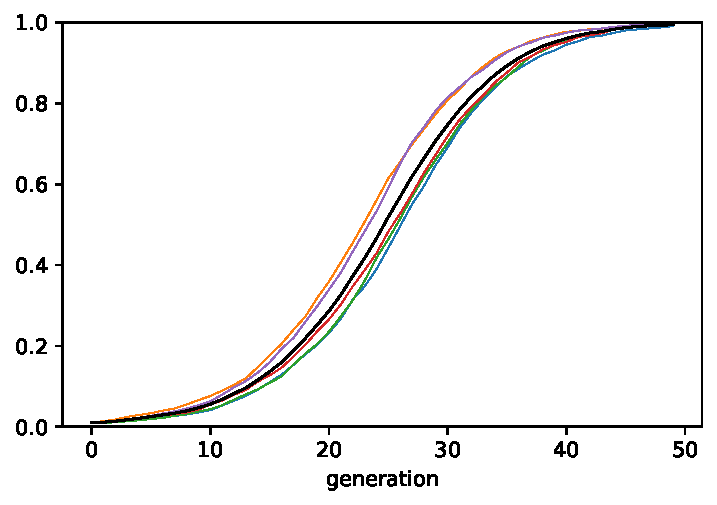
\includegraphics{chapter08_files/figure-pdf/cell-5-output-1.pdf}

}

\end{figure}

\begin{Shaded}
\begin{Highlighting}[]
\NormalTok{data\_model }\OperatorTok{=}\NormalTok{ vertical\_transmission(N}\OperatorTok{=}\DecValTok{10\_000}\NormalTok{, p\_0}\OperatorTok{=}\FloatTok{0.1}\NormalTok{, b}\OperatorTok{=}\FloatTok{0.5}\NormalTok{,t\_max}\OperatorTok{=}\DecValTok{50}\NormalTok{, r\_max}\OperatorTok{=}\DecValTok{5}\NormalTok{)}
\NormalTok{plot\_multiple\_runs(data\_model)}
\end{Highlighting}
\end{Shaded}

\begin{figure}[H]

{\centering 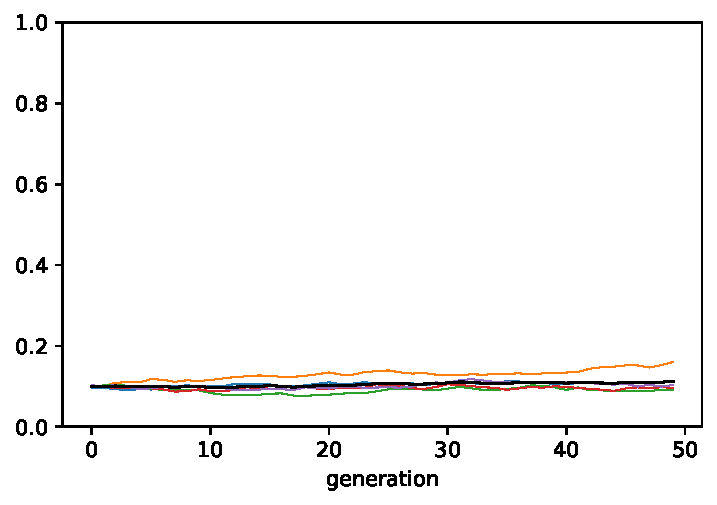
\includegraphics{chapter08_files/figure-pdf/cell-6-output-1.pdf}

}

\end{figure}

\begin{tcolorbox}[enhanced jigsaw, arc=.35mm, colbacktitle=quarto-callout-warning-color!10!white, colback=white, breakable, toprule=.15mm, title=\textcolor{quarto-callout-warning-color}{\faExclamationTriangle}\hspace{0.5em}{Warning}, left=2mm, bottomtitle=1mm, toptitle=1mm, leftrule=.75mm, opacitybacktitle=0.6, titlerule=0mm, opacityback=0, rightrule=.15mm, bottomrule=.15mm, coltitle=black, colframe=quarto-callout-warning-color-frame]

The code below is not yet correct and runs very slowly.

\end{tcolorbox}

\begin{Shaded}
\begin{Highlighting}[]
\KeywordTok{def}\NormalTok{ vertical\_horizontal\_transmission(N, p\_0, b, n, g, t\_max, r\_max):}
    \CommentTok{\# Create the output DataFrame}
\NormalTok{    output }\OperatorTok{=}\NormalTok{ pd.DataFrame(\{}
        \StringTok{"generation"}\NormalTok{ : np.tile(np.arange(t\_max), r\_max),}
        \StringTok{"p"}\NormalTok{ : [ np.nan ] }\OperatorTok{*}\NormalTok{ t\_max }\OperatorTok{*}\NormalTok{ r\_max,}
        \StringTok{"run"}\NormalTok{ : np.repeat(np.arange(r\_max), t\_max)}
\NormalTok{    \})}

    \ControlFlowTok{for}\NormalTok{ r }\KeywordTok{in} \BuiltInTok{range}\NormalTok{(r\_max):}
        \CommentTok{\# Create first generation}
\NormalTok{        population }\OperatorTok{=}\NormalTok{ pd.DataFrame(\{}\StringTok{"trait"}\NormalTok{: rng.choice([}\StringTok{"A"}\NormalTok{, }\StringTok{"B"}\NormalTok{], size}\OperatorTok{=}\NormalTok{N, replace}\OperatorTok{=}\VariableTok{True}\NormalTok{, p}\OperatorTok{=}\NormalTok{[p\_0, }\DecValTok{1} \OperatorTok{{-}}\NormalTok{ p\_0])\})}

        \CommentTok{\# Add first generation\textquotesingle{}s p for run r}
\NormalTok{        output.loc[ r }\OperatorTok{*}\NormalTok{ t\_max, }\StringTok{"p"}\NormalTok{] }\OperatorTok{=}\NormalTok{ population[ population[}\StringTok{"trait"}\NormalTok{] }\OperatorTok{==} \StringTok{"A"}\NormalTok{ ].shape[}\DecValTok{0}\NormalTok{] }\OperatorTok{/}\NormalTok{ N}

        \CommentTok{\# For each generation }
        \ControlFlowTok{for}\NormalTok{ t }\KeywordTok{in}\NormalTok{ tqdm(}\BuiltInTok{range}\NormalTok{(t\_max)):}
            \CommentTok{\#\#\# Vertical transmission =========================================================}

            \CommentTok{\# Copy individuals to previous\_population DataFrame}
\NormalTok{            previous\_population }\OperatorTok{=}\NormalTok{ population.copy()}

            \CommentTok{\# randomly pick mothers and fathers}
\NormalTok{            mother }\OperatorTok{=}\NormalTok{ previous\_population[}\StringTok{"trait"}\NormalTok{].sample(N, replace}\OperatorTok{=}\VariableTok{True}\NormalTok{).reset\_index(drop}\OperatorTok{=}\VariableTok{True}\NormalTok{)}
\NormalTok{            father }\OperatorTok{=}\NormalTok{ previous\_population[}\StringTok{"trait"}\NormalTok{].sample(N, replace}\OperatorTok{=}\VariableTok{True}\NormalTok{).reset\_index(drop}\OperatorTok{=}\VariableTok{True}\NormalTok{)}

            \CommentTok{\# prepare next generation}
\NormalTok{            population }\OperatorTok{=}\NormalTok{ pd.DataFrame(\{}\StringTok{"trait"}\NormalTok{: [np.nan] }\OperatorTok{*}\NormalTok{ N \})}

            \CommentTok{\# Both parents are A, thus child adopts A}
\NormalTok{            both\_A }\OperatorTok{=}\NormalTok{ (mother }\OperatorTok{==} \StringTok{"A"}\NormalTok{) }\OperatorTok{\&}\NormalTok{ (father }\OperatorTok{==} \StringTok{"A"}\NormalTok{)}
            \CommentTok{\# if sum(both\_A) \textgreater{} 0:}
\NormalTok{            population.loc[both\_A,}\StringTok{"trait"}\NormalTok{] }\OperatorTok{=} \StringTok{"A"}

            \CommentTok{\# Both parents are A, thus child adopts A}
\NormalTok{            both\_B }\OperatorTok{=}\NormalTok{ (mother }\OperatorTok{==} \StringTok{"B"}\NormalTok{) }\OperatorTok{\&}\NormalTok{ (father }\OperatorTok{==} \StringTok{"B"}\NormalTok{)}
            \CommentTok{\# if sum(both\_B) \textgreater{} 0:}
\NormalTok{            population.loc[both\_B,}\StringTok{"trait"}\NormalTok{] }\OperatorTok{=} \StringTok{"B"}

            \CommentTok{\# If any empty NA slots are present (i.e. one A and one B parent) they adopt A with probability b}
\NormalTok{            remaining }\OperatorTok{=}\NormalTok{ rng.choice([}\StringTok{"A"}\NormalTok{, }\StringTok{"B"}\NormalTok{], size}\OperatorTok{=}\NormalTok{population[}\StringTok{"trait"}\NormalTok{].isna().}\BuiltInTok{sum}\NormalTok{(), replace}\OperatorTok{=}\VariableTok{True}\NormalTok{, p}\OperatorTok{=}\NormalTok{[b, }\DecValTok{1} \OperatorTok{{-}}\NormalTok{ b])}
\NormalTok{            population.loc[population[}\StringTok{"trait"}\NormalTok{].isna(),}\StringTok{"trait"}\NormalTok{] }\OperatorTok{=}\NormalTok{ remaining}
            
            \CommentTok{\# Get p and put it into output slot for this generation t and run r}
\NormalTok{            output.loc[r }\OperatorTok{*}\NormalTok{ t\_max }\OperatorTok{+}\NormalTok{ t, }\StringTok{"p"}\NormalTok{] }\OperatorTok{=}\NormalTok{ population[ population[}\StringTok{"trait"}\NormalTok{] }\OperatorTok{==} \StringTok{"A"}\NormalTok{ ].shape[}\DecValTok{0}\NormalTok{] }\OperatorTok{/}\NormalTok{ N}

            \CommentTok{\#\# Horizontal transmission =========================================================}

\NormalTok{            previous\_population }\OperatorTok{=}\NormalTok{ population.copy()}
            \CommentTok{\# \# N\_B = number of Bs}
\NormalTok{            N\_B }\OperatorTok{=}\NormalTok{ previous\_population[previous\_population[}\StringTok{"trait"}\NormalTok{] }\OperatorTok{==} \StringTok{"B"}\NormalTok{].shape[}\DecValTok{0}\NormalTok{]}

            \CommentTok{\# if there are B individuals to switch, and n is not zero:}
            \ControlFlowTok{if}\NormalTok{ (N\_B }\OperatorTok{\textgreater{}} \DecValTok{0}\NormalTok{) }\OperatorTok{\&}\NormalTok{ (n }\OperatorTok{\textgreater{}} \DecValTok{0}\NormalTok{):}
                \CommentTok{\# for each B individual:}
                \ControlFlowTok{for}\NormalTok{ i }\KeywordTok{in} \BuiltInTok{range}\NormalTok{(N\_B):}
                    \CommentTok{\# Pick n demonstrators}
\NormalTok{                    demonstrator }\OperatorTok{=}\NormalTok{ previous\_population[}\StringTok{"trait"}\NormalTok{].sample(n, replace}\OperatorTok{=}\VariableTok{True}\NormalTok{)}
                    \CommentTok{\# Get probability g }
\NormalTok{                    copy\_ }\OperatorTok{=}\NormalTok{ rng.choice([}\VariableTok{True}\NormalTok{, }\VariableTok{False}\NormalTok{], n, p}\OperatorTok{=}\NormalTok{[g, }\DecValTok{1} \OperatorTok{{-}}\NormalTok{ g], replace}\OperatorTok{=}\VariableTok{True}\NormalTok{)}
                    \CommentTok{\# if any demonstrators with A are to be copied:}
                    \ControlFlowTok{if} \BuiltInTok{sum}\NormalTok{((demonstrator }\OperatorTok{==} \StringTok{"A"}\NormalTok{) }\OperatorTok{\&}\NormalTok{ (copy\_)) }\OperatorTok{\textgreater{}} \DecValTok{0}\NormalTok{:}
                      \CommentTok{\# The B individual switches to A }
                      \CommentTok{\# }\AlertTok{TODO}\CommentTok{: Here\textquotesingle{}s the bug!}
\NormalTok{                      population[previous\_population[}\StringTok{"trait"}\NormalTok{] }\OperatorTok{==} \StringTok{"B"}\NormalTok{].at[i, }\StringTok{"trait"}\NormalTok{] }\OperatorTok{=} \StringTok{"A"}

\NormalTok{            next\_population }\OperatorTok{=}\NormalTok{ population.copy()}
            \CommentTok{\# \# N\_B = number of Bs}
\NormalTok{            N\_B }\OperatorTok{=}\NormalTok{ next\_population[next\_population[}\StringTok{"trait"}\NormalTok{] }\OperatorTok{==} \StringTok{"B"}\NormalTok{].shape[}\DecValTok{0}\NormalTok{]}

            \CommentTok{\# if there are B individuals to switch, and n is not zero:}
            \ControlFlowTok{if}\NormalTok{ (N\_B }\OperatorTok{\textgreater{}} \DecValTok{0}\NormalTok{) }\OperatorTok{\&}\NormalTok{ (n }\OperatorTok{\textgreater{}} \DecValTok{0}\NormalTok{):}
                \CommentTok{\# for each B individual:}
                \ControlFlowTok{for}\NormalTok{ i }\KeywordTok{in} \BuiltInTok{range}\NormalTok{(N\_B):}
                    \CommentTok{\# Pick n demonstrators}
\NormalTok{                    demonstrator }\OperatorTok{=}\NormalTok{ population[}\StringTok{"trait"}\NormalTok{].sample(n, replace}\OperatorTok{=}\VariableTok{True}\NormalTok{)}
                    \CommentTok{\# Get probability g }
\NormalTok{                    copy\_ }\OperatorTok{=}\NormalTok{ rng.choice([}\VariableTok{True}\NormalTok{, }\VariableTok{False}\NormalTok{], n, p}\OperatorTok{=}\NormalTok{[g, }\DecValTok{1} \OperatorTok{{-}}\NormalTok{ g], replace}\OperatorTok{=}\VariableTok{True}\NormalTok{)}
                    \CommentTok{\# if any demonstrators with A are to be copied:}
                    \ControlFlowTok{if} \BuiltInTok{sum}\NormalTok{((demonstrator }\OperatorTok{==} \StringTok{"A"}\NormalTok{) }\OperatorTok{\&}\NormalTok{ (copy\_)) }\OperatorTok{\textgreater{}} \DecValTok{0}\NormalTok{:}
                      \CommentTok{\# The B individual switches to A }
\NormalTok{                      next\_population[next\_population[}\StringTok{"trait"}\NormalTok{] }\OperatorTok{==} \StringTok{"B"}\NormalTok{].at[i, }\StringTok{"trait"}\NormalTok{] }\OperatorTok{=} \StringTok{"A"}

            \CommentTok{\# Get p and put it into output slot for this generation t and run r}
\NormalTok{            output.loc[r }\OperatorTok{*}\NormalTok{ t\_max }\OperatorTok{+}\NormalTok{ t, }\StringTok{"p"}\NormalTok{] }\OperatorTok{=}\NormalTok{ next\_population[ next\_population[}\StringTok{"trait"}\NormalTok{] }\OperatorTok{==} \StringTok{"A"}\NormalTok{ ].shape[}\DecValTok{0}\NormalTok{] }\OperatorTok{/}\NormalTok{ N}

    \ControlFlowTok{return}\NormalTok{ output}
\end{Highlighting}
\end{Shaded}

\begin{Shaded}
\begin{Highlighting}[]
\NormalTok{vertical\_horizontal\_transmission(N}\OperatorTok{=}\DecValTok{1000}\NormalTok{, p\_0}\OperatorTok{=}\FloatTok{0.01}\NormalTok{, b}\OperatorTok{=}\FloatTok{0.5}\NormalTok{, n}\OperatorTok{=}\DecValTok{5}\NormalTok{, g}\OperatorTok{=}\FloatTok{0.1}\NormalTok{, t\_max}\OperatorTok{=}\DecValTok{10}\NormalTok{, r\_max}\OperatorTok{=}\DecValTok{1}\NormalTok{)}
\end{Highlighting}
\end{Shaded}

\begin{tabular}{lrrr}
\toprule
{} &  generation &      p &  run \\
\midrule
0 &           0 &  0.011 &    0 \\
1 &           1 &  0.014 &    0 \\
2 &           2 &  0.007 &    0 \\
3 &           3 &  0.004 &    0 \\
4 &           4 &  0.003 &    0 \\
5 &           5 &  0.004 &    0 \\
6 &           6 &  0.005 &    0 \\
7 &           7 &  0.008 &    0 \\
8 &           8 &  0.006 &    0 \\
9 &           9 &  0.011 &    0 \\
\bottomrule
\end{tabular}

\begin{Shaded}
\begin{Highlighting}[]
\CommentTok{\# data\_model = vertical\_horizontal\_transmission(N=5\_000, p\_0=0.01, b=0.5, n=5, g=0.1, t\_max=50, r\_max=2)}
\CommentTok{\# plot\_multiple\_runs(data\_model)}
\end{Highlighting}
\end{Shaded}

\hypertarget{sec-multiple-traits}{%
\chapter{The multiple traits model}\label{sec-multiple-traits}}

\begin{Shaded}
\begin{Highlighting}[]
\ImportTok{import}\NormalTok{ pandas }\ImportTok{as}\NormalTok{ pd}
\ImportTok{import}\NormalTok{ numpy }\ImportTok{as}\NormalTok{ np}
\NormalTok{rng }\OperatorTok{=}\NormalTok{ np.random.default\_rng()}

\ImportTok{import}\NormalTok{ matplotlib.pyplot }\ImportTok{as}\NormalTok{ plt}

\NormalTok{N }\OperatorTok{=} \DecValTok{100}
\NormalTok{population }\OperatorTok{=}\NormalTok{ pd.DataFrame(}
\NormalTok{    \{}\StringTok{"trait"}\NormalTok{ : rng.integers(N, size}\OperatorTok{=}\NormalTok{N)\}}
\NormalTok{)}
\end{Highlighting}
\end{Shaded}

\begin{Shaded}
\begin{Highlighting}[]
\NormalTok{population.head()}
\end{Highlighting}
\end{Shaded}

\begin{verbatim}
/home/fmoss/.local/lib/python3.10/site-packages/IPython/core/formatters.py:343: FutureWarning: In future versions `DataFrame.to_latex` is expected to utilise the base implementation of `Styler.to_latex` for formatting and rendering. The arguments signature may therefore change. It is recommended instead to use `DataFrame.style.to_latex` which also contains additional functionality.
  return method()
\end{verbatim}

\begin{tabular}{lr}
\toprule
{} &  trait \\
\midrule
0 &     77 \\
1 &     48 \\
2 &     22 \\
3 &     93 \\
4 &     75 \\
\bottomrule
\end{tabular}

\begin{Shaded}
\begin{Highlighting}[]
\KeywordTok{def}\NormalTok{ multiple\_traits(N, t\_max):}
\NormalTok{    output }\OperatorTok{=}\NormalTok{ pd.DataFrame(\{}
        \StringTok{"trait"}\NormalTok{ : np.repeat(np.arange(N), t\_max),}
        \StringTok{"generation"}\NormalTok{ : np.tile(np.arange(t\_max), N),}
        \StringTok{"p"}\NormalTok{ : [ np.nan ] }\OperatorTok{*}\NormalTok{ t\_max }\OperatorTok{*}\NormalTok{ N,}
\NormalTok{    \})}

    \CommentTok{\# Create first generation }
\NormalTok{    population }\OperatorTok{=}\NormalTok{ pd.DataFrame(\{}\StringTok{"trait"}\NormalTok{ : rng.integers(N, size}\OperatorTok{=}\NormalTok{N)\})}

    \CommentTok{\# Add first generation\textquotesingle{}s p for all traits}
\NormalTok{    output.loc[output[}\StringTok{"generation"}\NormalTok{] }\OperatorTok{==} \DecValTok{0}\NormalTok{, }\StringTok{"p"}\NormalTok{] }\OperatorTok{=}\NormalTok{ population[}\StringTok{"trait"}\NormalTok{].value\_counts(normalize}\OperatorTok{=}\VariableTok{True}\NormalTok{).reindex(}\BuiltInTok{range}\NormalTok{(N)).fillna(}\FloatTok{0.}\NormalTok{).values}

    \ControlFlowTok{for}\NormalTok{ t }\KeywordTok{in} \BuiltInTok{range}\NormalTok{(t\_max):}
        \CommentTok{\# Copy individuals to previous\_population DataFrame}
\NormalTok{        previous\_population }\OperatorTok{=}\NormalTok{ population.copy()}

        \CommentTok{\# Randomly copy from previous generation}
\NormalTok{        population }\OperatorTok{=}\NormalTok{ pd.DataFrame(\{}\StringTok{"trait"}\NormalTok{ : previous\_population[}\StringTok{"trait"}\NormalTok{].sample(N, replace}\OperatorTok{=}\VariableTok{True}\NormalTok{)\})}

        \CommentTok{\# Get p for all traits and put it into output slot for this generation t}
\NormalTok{        output.loc[output[}\StringTok{"generation"}\NormalTok{] }\OperatorTok{==}\NormalTok{ t, }\StringTok{"p"}\NormalTok{] }\OperatorTok{=}\NormalTok{ population[}\StringTok{"trait"}\NormalTok{].value\_counts(normalize}\OperatorTok{=}\VariableTok{True}\NormalTok{).reindex(}\BuiltInTok{range}\NormalTok{(N)).fillna(}\FloatTok{0.}\NormalTok{).values}

    \ControlFlowTok{return}\NormalTok{ output}
\end{Highlighting}
\end{Shaded}

\begin{Shaded}
\begin{Highlighting}[]
\KeywordTok{def}\NormalTok{ plot\_multiple\_traits(data\_model):}
\NormalTok{    ps }\OperatorTok{=}\NormalTok{ []}
    \ControlFlowTok{for}\NormalTok{ \_, g }\KeywordTok{in}\NormalTok{ data\_model.groupby(}\StringTok{"trait"}\NormalTok{):}
\NormalTok{        x }\OperatorTok{=}\NormalTok{ g[}\StringTok{"generation"}\NormalTok{]}
\NormalTok{        ps.append(g[}\StringTok{"p"}\NormalTok{])}

\NormalTok{    plt.stackplot(x, }\OperatorTok{*}\NormalTok{ps, cmap}\OperatorTok{=}\StringTok{"tab20"}\NormalTok{)}
\NormalTok{    plt.margins(}\FloatTok{0.}\NormalTok{)}
\NormalTok{    plt.show()}
\end{Highlighting}
\end{Shaded}

\begin{Shaded}
\begin{Highlighting}[]
\NormalTok{data\_model }\OperatorTok{=}\NormalTok{ multiple\_traits(N}\OperatorTok{=}\DecValTok{100}\NormalTok{, t\_max}\OperatorTok{=}\DecValTok{200}\NormalTok{)}
\NormalTok{plot\_multiple\_traits(data\_model)}
\end{Highlighting}
\end{Shaded}

\begin{figure}[H]

{\centering 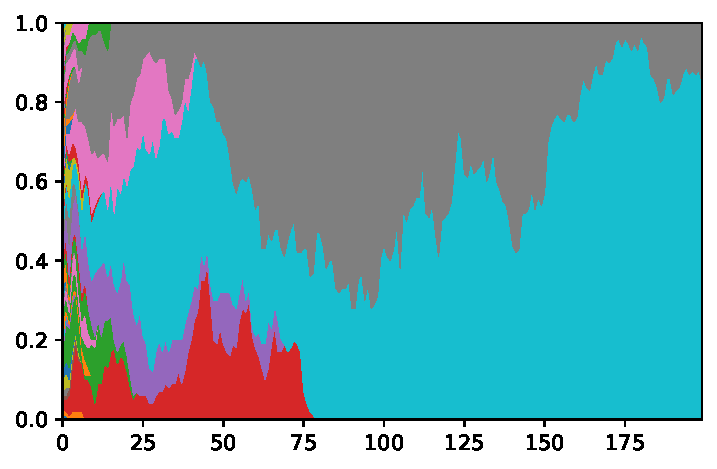
\includegraphics{chapter09_files/figure-pdf/cell-6-output-1.pdf}

}

\end{figure}

\begin{Shaded}
\begin{Highlighting}[]
\NormalTok{data\_model }\OperatorTok{=}\NormalTok{ multiple\_traits(N}\OperatorTok{=}\DecValTok{100}\NormalTok{, t\_max}\OperatorTok{=}\DecValTok{1000}\NormalTok{)}
\NormalTok{plot\_multiple\_traits(data\_model)}
\end{Highlighting}
\end{Shaded}

\begin{figure}[H]

{\centering 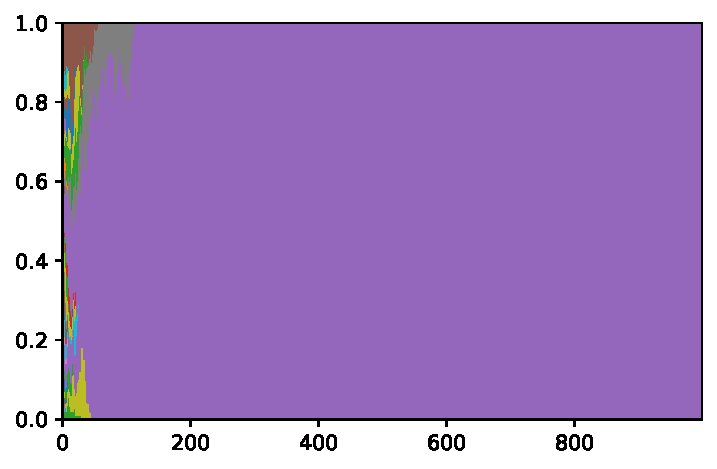
\includegraphics{chapter09_files/figure-pdf/cell-7-output-1.pdf}

}

\end{figure}

\hypertarget{introducing-innovation}{%
\section{Introducing innovation}\label{introducing-innovation}}

\part{Advanced topics}

\hypertarget{modeling-document-traditions}{%
\chapter{Modeling document
traditions}\label{modeling-document-traditions}}

Here, we show how one can use cultural evolution methods to model the
histories of manuscripts. This is based on a phylogenetic analysis of a
Prelude by Orlando Gibbons (Windram et al., 2014).

\hypertarget{context}{%
\section{Context}\label{context}}

Mutations create new traditions \protect\hyperlink{todo}{TODO}

\hypertarget{data-and-coding}{%
\section{Data and coding}\label{data-and-coding}}

We use the same data as in (Windram et al., 2014)\footnote{I am grateful
  to Heather Windram for providing the data and to Francis Windram for
  helping me to parse it properly.}

This is a case of a qualitative encoding, because the features were
manually chosen and encoded according to the expert's opinion.

In the context of this chapter, we will rely on implementations of
several algorithms in the \emph{BioPython} library. We also implot
\texttt{matplotlib} for visualization.

\begin{Shaded}
\begin{Highlighting}[]
\ImportTok{from}\NormalTok{ Bio }\ImportTok{import}\NormalTok{ SeqIO, AlignIO, Phylo}
\ImportTok{from}\NormalTok{ Bio.Phylo.TreeConstruction }\ImportTok{import}\NormalTok{ DistanceCalculator, DistanceTreeConstructor}

\ImportTok{import}\NormalTok{ matplotlib}
\ImportTok{import}\NormalTok{ matplotlib.pyplot }\ImportTok{as}\NormalTok{ plt}
\end{Highlighting}
\end{Shaded}

The data codings are stored in the file \texttt{gibbons\_prelude.nex} in
the \href{https://en.wikipedia.org/wiki/Nexus_file}{NEXUS format}.
First, let's have a look at the file's contents:

\begin{Shaded}
\begin{Highlighting}[]
\BuiltInTok{file} \OperatorTok{=} \StringTok{"data/gibbons\_prelude.nex"}
\ControlFlowTok{with} \BuiltInTok{open}\NormalTok{(}\BuiltInTok{file}\NormalTok{) }\ImportTok{as}\NormalTok{ f:}
    \ControlFlowTok{for}\NormalTok{ line }\KeywordTok{in}\NormalTok{ f.readlines():}
\NormalTok{        line }\OperatorTok{=}\NormalTok{ line.rstrip(}\StringTok{"}\CharTok{\textbackslash{}n}\StringTok{"}\NormalTok{) }\CommentTok{\# remove trailing line breaks}
        \BuiltInTok{print}\NormalTok{(line[:}\DecValTok{65}\NormalTok{])}
\end{Highlighting}
\end{Shaded}

\begin{verbatim}
#NEXUS
[! 01-Nov-2013 - with taxanames 07-Feb-2023]
BEGIN taxa;
    DIMENSIONS NTAX=16;
    TAXLABELS
    [1] Parthenia
    [2] Lcm2093
    [3] Och47
    [4] Och89
    [5] Lbl31403
    [6] NYp5612
    [7] Cfm653
    [8] Lbl22099
    [9] LynarA2
    [10] Lbl23623i
    [11] Lbl23623ii
    [12] PcRes1186bisI
    [13] LblMus1
    [14] TnN335
    [15] Dolmetsch
    [16] Filmer17
    
;
END;
BEGIN characters;
    dimensions nchar=610;
    format
        datatype=standard
        missing=?
        respectcase SYMBOLS="0123456789abcdefghijklmnopqrstuvwxyz";
    matrix
Parthenia       000000000000000000000000000000000000000?000000000
Lcm2093         110010100000000000000000000000000001000?000000011
Och47           00002110110011110110111?1010100010010010000000012
Och89           000031102001000000000000000020000011112?100000010
Lbl31403        220010?10000200000010000010120000002022?100000013
NYp5612         33000020110000000000000000000000001?000?0000000?0
Cfm653          22110011110011110210121111?031?01001022?00100??11
Lbl22099        401000113?11111102101211111041011001022?11?100013
LynarA2         000000211100000000000000000000000013000?000000023
Lbl23623i       540001?000101121100000000000000001100?2?001110001
Lbl23623ii      640001?01110111100000000000000000011002?001110011
PcRes1186bisI   200000110000112113000300000020000001022?100000011
LblMus1         2100001000011111011014001010500010010010000000011
TnN335          750100111100111104101511111031001001002?001000013
Dolmetsch       811000100001111100000000021061000001002?001000011
Filmer17        2110001000002000000000000000200000010011000000011
    ;
END;
\end{verbatim}

The file's structure is very clear. In the header, it declares its
format (\texttt{\#NEXUS}) along with some metadata, and then lists the
16 `taxa' (the original \emph{Parthenia} and its different copies). It
further describes the encoding scheme, namely which \texttt{SYMBOLS} can
be used (integers from 0-9 as well as lowercase roman letters), and that
the \texttt{?} symbol will be used for missing data. We also can see
that the dimensionality is \texttt{nchar=610}, meaning that the encoding
emcompasses 610 different features.

Let's read in the file using BioPython's built-in parser and print the
names of all manuscripts:

\begin{Shaded}
\begin{Highlighting}[]
\ControlFlowTok{for}\NormalTok{ manuscript }\KeywordTok{in}\NormalTok{ SeqIO.parse(}\BuiltInTok{file}\NormalTok{, }\BuiltInTok{format}\OperatorTok{=}\StringTok{"nexus"}\NormalTok{):}
    \BuiltInTok{print}\NormalTok{(manuscript.name) }
\end{Highlighting}
\end{Shaded}

\begin{verbatim}
Parthenia
Lcm2093
Och47
Och89
Lbl31403
NYp5612
Cfm653
Lbl22099
LynarA2
Lbl23623i
Lbl23623ii
PcRes1186bisI
LblMus1
TnN335
Dolmetsch
Filmer17
\end{verbatim}

\hypertarget{sequence-alignment}{%
\section{Sequence alignment}\label{sequence-alignment}}

Each manuscript containing Gibbon's Prelude is encoded as a string of
characters (see above). In order to find deviations, mutations, and
errors in the sequences, we will find best alignments of the manuscript
encodings using BioPython. While the alignments here rely purely on
visual and philological features of the text, this methodology has also
been successfully applied to melodic variations (Savage et al., 2022).

\begin{Shaded}
\begin{Highlighting}[]
\NormalTok{alignments }\OperatorTok{=} \BuiltInTok{next}\NormalTok{(AlignIO.parse(}\BuiltInTok{file}\NormalTok{, }\BuiltInTok{format}\OperatorTok{=}\StringTok{"nexus"}\NormalTok{))}
\BuiltInTok{print}\NormalTok{(alignments[:}\DecValTok{3}\NormalTok{])}
\end{Highlighting}
\end{Shaded}

\begin{verbatim}
Alignment with 3 rows and 610 columns
[{'t': 'std', 'd': ['0']}, {'t': 'std', 'd': ['0']}, {'t': 'std', 'd': ['0']}, {'t': 'std', 'd': ['0']}, {'t': 'std', 'd': ['0']}, {'t': 'std', 'd': ['0']}, {'t': 'std', 'd': ['0']}, {'t': 'std', 'd': ['0']}, {'t': 'std', 'd': ['0']}, {'t': 'std', 'd': ['0']}, {'t': 'std', 'd': ['0']}, {'t': 'std', 'd': ['0']}, {'t': 'std', 'd': ['0']}, {'t': 'std', 'd': ['0']}, {'t': 'std', 'd': ['0']}, {'t': 'std', 'd': ['0']}, {'t': 'std', 'd': ['0']}, {'t': 'std', 'd': ['0']}, {'t': 'std', 'd': ['0']}, {'t': 'std', 'd': ['0']}, {'t': 'std', 'd': ['0']}, {'t': 'std', 'd': ['0']}, {'t': 'std', 'd': ['0']}, {'t': 'std', 'd': ['0']}, {'t': 'std', 'd': ['0']}, {'t': 'std', 'd': ['0']}, {'t': 'std', 'd': ['0']}, {'t': 'std', 'd': ['0']}, {'t': 'std', 'd': ['0']}, {'t': 'std', 'd': ['0']}, {'t': 'std', 'd': ['0']}, {'t': 'std', 'd': ['0']}, {'t': 'std', 'd': ['0']}, {'t': 'std', 'd': ['0']}, {'t': 'std', 'd': ['0']}, {'t': 'std', 'd': ['0']}, {'t': 'std', 'd': ['0']}, {'t': 'std', 'd': ['0']}, {'t': 'std', 'd': ['0']}, {'t': 'std', 'd': ['?']}, {'t': 'std', 'd': ['0']}, {'t': 'std', 'd': ['0']}, {'t': 'std', 'd': ['0']}, {'t': 'std', 'd': ['0']}]...[{'t': 'std', 'd': ['0']}, {'t': 'std', 'd': ['0']}, {'t': 'std', 'd': ['0']}] Parthenia
[{'t': 'std', 'd': ['1']}, {'t': 'std', 'd': ['1']}, {'t': 'std', 'd': ['0']}, {'t': 'std', 'd': ['0']}, {'t': 'std', 'd': ['1']}, {'t': 'std', 'd': ['0']}, {'t': 'std', 'd': ['1']}, {'t': 'std', 'd': ['0']}, {'t': 'std', 'd': ['0']}, {'t': 'std', 'd': ['0']}, {'t': 'std', 'd': ['0']}, {'t': 'std', 'd': ['0']}, {'t': 'std', 'd': ['0']}, {'t': 'std', 'd': ['0']}, {'t': 'std', 'd': ['0']}, {'t': 'std', 'd': ['0']}, {'t': 'std', 'd': ['0']}, {'t': 'std', 'd': ['0']}, {'t': 'std', 'd': ['0']}, {'t': 'std', 'd': ['0']}, {'t': 'std', 'd': ['0']}, {'t': 'std', 'd': ['0']}, {'t': 'std', 'd': ['0']}, {'t': 'std', 'd': ['0']}, {'t': 'std', 'd': ['0']}, {'t': 'std', 'd': ['0']}, {'t': 'std', 'd': ['0']}, {'t': 'std', 'd': ['0']}, {'t': 'std', 'd': ['0']}, {'t': 'std', 'd': ['0']}, {'t': 'std', 'd': ['0']}, {'t': 'std', 'd': ['0']}, {'t': 'std', 'd': ['0']}, {'t': 'std', 'd': ['0']}, {'t': 'std', 'd': ['0']}, {'t': 'std', 'd': ['1']}, {'t': 'std', 'd': ['0']}, {'t': 'std', 'd': ['0']}, {'t': 'std', 'd': ['0']}, {'t': 'std', 'd': ['?']}, {'t': 'std', 'd': ['0']}, {'t': 'std', 'd': ['0']}, {'t': 'std', 'd': ['0']}, {'t': 'std', 'd': ['0']}]...[{'t': 'std', 'd': ['0']}, {'t': 'std', 'd': ['?']}, {'t': 'std', 'd': ['1']}] Lcm2093
[{'t': 'std', 'd': ['0']}, {'t': 'std', 'd': ['0']}, {'t': 'std', 'd': ['0']}, {'t': 'std', 'd': ['0']}, {'t': 'std', 'd': ['2']}, {'t': 'std', 'd': ['1']}, {'t': 'std', 'd': ['1']}, {'t': 'std', 'd': ['0']}, {'t': 'std', 'd': ['1']}, {'t': 'std', 'd': ['1']}, {'t': 'std', 'd': ['0']}, {'t': 'std', 'd': ['0']}, {'t': 'std', 'd': ['1']}, {'t': 'std', 'd': ['1']}, {'t': 'std', 'd': ['1']}, {'t': 'std', 'd': ['1']}, {'t': 'std', 'd': ['0']}, {'t': 'std', 'd': ['1']}, {'t': 'std', 'd': ['1']}, {'t': 'std', 'd': ['0']}, {'t': 'std', 'd': ['1']}, {'t': 'std', 'd': ['1']}, {'t': 'std', 'd': ['1']}, {'t': 'std', 'd': ['?']}, {'t': 'std', 'd': ['1']}, {'t': 'std', 'd': ['0']}, {'t': 'std', 'd': ['1']}, {'t': 'std', 'd': ['0']}, {'t': 'std', 'd': ['1']}, {'t': 'std', 'd': ['0']}, {'t': 'std', 'd': ['0']}, {'t': 'std', 'd': ['0']}, {'t': 'std', 'd': ['1']}, {'t': 'std', 'd': ['0']}, {'t': 'std', 'd': ['0']}, {'t': 'std', 'd': ['1']}, {'t': 'std', 'd': ['0']}, {'t': 'std', 'd': ['0']}, {'t': 'std', 'd': ['1']}, {'t': 'std', 'd': ['0']}, {'t': 'std', 'd': ['0']}, {'t': 'std', 'd': ['0']}, {'t': 'std', 'd': ['0']}, {'t': 'std', 'd': ['0']}]...[{'t': 'std', 'd': ['0']}, {'t': 'std', 'd': ['1']}, {'t': 'std', 'd': ['1']}] Och47
\end{verbatim}

\hypertarget{constructing-a-possible-lineage}{%
\section{Constructing a possible
lineage}\label{constructing-a-possible-lineage}}

We are now in the position to create a possible hereditance system out
of these alignments because we can use these closest alignments to
determine pairwise distances between the sequences.

\begin{Shaded}
\begin{Highlighting}[]
\NormalTok{calculator }\OperatorTok{=}\NormalTok{ DistanceCalculator(model}\OperatorTok{=}\StringTok{"identity"}\NormalTok{)}
\NormalTok{distance\_matrix }\OperatorTok{=}\NormalTok{ calculator.get\_distance(alignments)}
\NormalTok{constructor }\OperatorTok{=}\NormalTok{ DistanceTreeConstructor(calculator)}
\end{Highlighting}
\end{Shaded}

From this constructor, we can now build a tree:

\begin{Shaded}
\begin{Highlighting}[]
\NormalTok{tree }\OperatorTok{=}\NormalTok{ constructor.build\_tree(alignments)}
\BuiltInTok{print}\NormalTok{(tree)}
\end{Highlighting}
\end{Shaded}

\begin{verbatim}
Tree(rooted=False)
    Clade(branch_length=0, name='Inner14')
        Clade(branch_length=0.020120389344262246, name='Inner12')
            Clade(branch_length=0.08942964480874313, name='Inner7')
                Clade(branch_length=0.3522540983606557, name='Lbl31403')
                Clade(branch_length=0.12725409836065588, name='Inner2')
                    Clade(branch_length=0.2826292559899118, name='Filmer17')
                    Clade(branch_length=0.13868221941992426, name='Och89')
            Clade(branch_length=0.22552937158469957, name='Inner1')
                Clade(branch_length=0.10017564402810297, name='NYp5612')
                Clade(branch_length=0.09162763466042156, name='Parthenia')
        Clade(branch_length=0.005033299180327883, name='Inner13')
            Clade(branch_length=0.021810963114754167, name='Inner11')
                Clade(branch_length=0.11976178278688522, name='Inner6')
                    Clade(branch_length=0.287431693989071, name='LblMus1')
                    Clade(branch_length=0.23060109289617492, name='Lbl22099')
                Clade(branch_length=0.01732838114754097, name='Inner10')
                    Clade(branch_length=0.3853483606557378, name='Cfm653')
                    Clade(branch_length=0.13186475409836057, name='Inner4')
                        Clade(branch_length=0.18412816691505207, name='TnN335')
                        Clade(branch_length=0.2535767511177348, name='Och47')
            Clade(branch_length=0.03418288934426228, name='Inner9')
                Clade(branch_length=0.06726434426229502, name='Inner8')
                    Clade(branch_length=0.2635538641686183, name='PcRes1186bisI')
                    Clade(branch_length=0.26595433255269324, name='LynarA2')
                Clade(branch_length=0.19298155737704922, name='Inner3')
                    Clade(branch_length=0.23695355191256845, name='Dolmetsch')
                    Clade(branch_length=0.08763661202185774, name='Lcm2093')
        Clade(branch_length=0.13326075819672134, name='Inner5')
            Clade(branch_length=0.28704918032786886, name='Lbl23623ii')
            Clade(branch_length=0.18836065573770489, name='Lbl23623i')
\end{verbatim}

The Phylo library provides a convenient function to plot this tree:

\begin{Shaded}
\begin{Highlighting}[]
\ControlFlowTok{for}\NormalTok{ clade }\KeywordTok{in}\NormalTok{ tree.get\_nonterminals():}
\NormalTok{    clade.name }\OperatorTok{=} \StringTok{""}
\NormalTok{fig }\OperatorTok{=}\NormalTok{ Phylo.draw(tree)}
\end{Highlighting}
\end{Shaded}

\begin{figure}[H]

{\centering 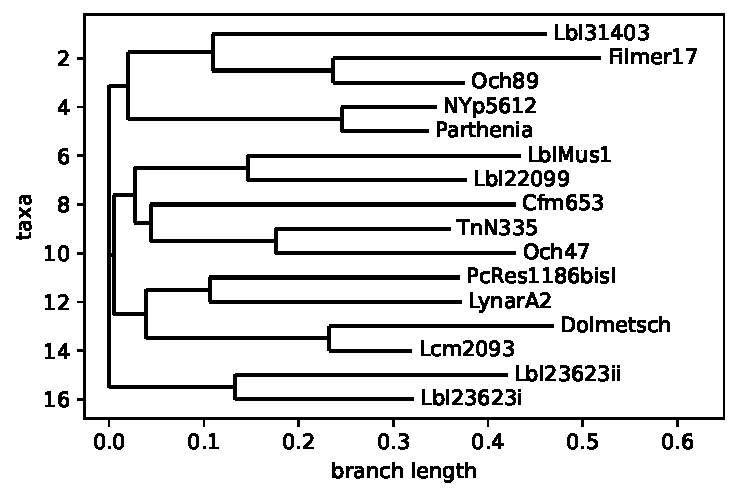
\includegraphics{document_traditions_files/figure-pdf/cell-8-output-1.pdf}

}

\end{figure}

\hypertarget{being-confident}{%
\section{Being confident}\label{being-confident}}

Use bootstrapping.

\hypertarget{conclusion}{%
\section{Conclusion}\label{conclusion}}

Briefly discuss NeighborNet graph and point to similar approach in
(Windram et al., 2022).

\hypertarget{the-usage-of-pitches-and-intervals}{%
\chapter{The usage of pitches and
intervals}\label{the-usage-of-pitches-and-intervals}}

\begin{itemize}
\tightlist
\item
  ``Cross-cultural data shows musical scales evolved to maximise
  imperfect fifths'' McBride \& Tlusty (2020)
\item
  ``The line of fifths and the co-evolution of tonal pitch-classes''
  (Moss et al., 2022)
\end{itemize}

\hypertarget{folk-tune-complexity}{%
\chapter{Folk tune complexity}\label{folk-tune-complexity}}

``The role of population size in folk tune complexity'' (Street et al.,
2022)

\hypertarget{music-communities}{%
\chapter{Music communities}\label{music-communities}}

studying the cultural evolution of electronic music

\hfill\break

``Phylogenetic reconstruction of the cultural evolution of electronic
music via dynamic community detection (1975--1999)'' (Youngblood et al.,
2021)

\hypertarget{style-evolution}{%
\chapter{Style evolution}\label{style-evolution}}

\begin{itemize}
\tightlist
\item
  ``Statistical Evolutionary Laws in Music Styles'' (Nakamura \& Kaneko,
  2019)
\item
  ``Investigating style evolution of Western classical music: A
  computational approach'' (Weiß et al., 2019)
\end{itemize}

\bookmarksetup{startatroot}

\hypertarget{sec-conclusion}{%
\chapter{Conclusion}\label{sec-conclusion}}

\hypertarget{what-can-cultural-evolution-tell-us-about-music}{%
\section{What can cultural evolution tell us about
music}\label{what-can-cultural-evolution-tell-us-about-music}}

\hypertarget{what-is-the-role-of-models-for-musicology}{%
\section{What is the role of models for
musicology}\label{what-is-the-role-of-models-for-musicology}}

\hypertarget{avenues-for-future-research}{%
\section{Avenues for future
research}\label{avenues-for-future-research}}

\bookmarksetup{startatroot}

\hypertarget{references}{%
\chapter*{References}\label{references}}
\addcontentsline{toc}{chapter}{References}

\markboth{References}{References}

\hypertarget{refs}{}
\begin{CSLReferences}{1}{0}
\leavevmode\vadjust pre{\hypertarget{ref-Acerbi2022}{}}%
Acerbi, A., Mesoudi, A., \& Smolla, M. (2022). \emph{{Individual-based
models of cultural evolution: A step-by-step guide using {R}}}.
Routledge. \url{https://acerbialberto.com/IBM-cultevo/}

\leavevmode\vadjust pre{\hypertarget{ref-Appiah2018_LiesThatBind}{}}%
Appiah, K. A. (2018). \emph{The {Lies} that {Bind}: {Rethinking
Identity}}. {W. W. Norton \& Company}.

\leavevmode\vadjust pre{\hypertarget{ref-Aunger2001_DarwinizingCultureStatus}{}}%
Aunger, R. (2001). \emph{Darwinizing {Culture}: {The Status} of
{Memetics} as a {Science}}. {Oxford University Press, USA}.
\url{http://gen.lib.rus.ec/book/index.php?md5=7329e2aa9adcddfed967088219426193}

\leavevmode\vadjust pre{\hypertarget{ref-Bentley2004_RandomDriftCulture}{}}%
Bentley, R. A., Hahn, M. W., \& Shennan, S. J. (2004). Random drift and
culture change. \emph{Proceedings of the Royal Society of London. Series
B: Biological Sciences}, \emph{271}(1547), 1443--1450.
\url{https://doi.org/10.1098/rspb.2004.2746}

\leavevmode\vadjust pre{\hypertarget{ref-Bishop2012_ModelbasedMachineLearning}{}}%
Bishop, C. M. (2012). Model-based machine learning. \emph{Philosophical
Transactions of The Royal Society A}, \emph{0222}(371).
\url{https://doi.org/10.1098/rsta.2012.0222}

\leavevmode\vadjust pre{\hypertarget{ref-Blackmore2000_MemeMachine}{}}%
Blackmore, S. (2000). \emph{The {Meme Machine}}. {Oxford University
Press}.

\leavevmode\vadjust pre{\hypertarget{ref-Boyd1985}{}}%
Boyd, R., \& Richerson, P. J. (1985). \emph{{Culture and the
Evolutionary Process}}. The University of Chicago Press.

\leavevmode\vadjust pre{\hypertarget{ref-Cavalli-Sforza1981_CulturalTransmissionEvolution}{}}%
Cavalli-Sforza, L. L., \& Feldman, M. W. (1981). \emph{Cultural
{Transmission} and {Evolution}}. {Princeton University Press}.

\leavevmode\vadjust pre{\hypertarget{ref-Cross2016_NatureMusicIts}{}}%
Cross, I. (2016). The nature of music and its evolution. In S. Hallam,
I. Cross, \& M. Thaut (Eds.), \emph{The {Oxford Handbook} of {Music
Psychology}} (2nd ed., pp. 1--20). {Oxford University Press}.
\url{https://doi.org/10.1093/oxfordhb/9780199298457.013.0001}

\leavevmode\vadjust pre{\hypertarget{ref-Dawkins1976_SelfishGenea}{}}%
Dawkins, R. (1976). \emph{The {Selfish Gene}}. {Oxford University
Press}.

\leavevmode\vadjust pre{\hypertarget{ref-Farrell2018_ComputationalModelingCognition}{}}%
Farrell, S., \& Lewandowsky, S. (2018). \emph{Computational {Modeling}
of {Cognition} and {Behavior}}. {Cambridge University Press}.
\url{https://doi.org/10.1017/CBO9781316272503}

\leavevmode\vadjust pre{\hypertarget{ref-Finkensiepforthcoming_MusicTheoryModeldriven}{}}%
Finkensiep, C., Neuwirth, M., \& Rohrmeier, M. (forthcoming). Music
{Theory} and {Model-driven Corpus Research}. In D. Shanahan, J. A.
Burgoyne, \& I. Quinn (Eds.), \emph{Oxford {Handbook} of {Music} and
{Corpus Studies}}. {Oxford University Press}.

\leavevmode\vadjust pre{\hypertarget{ref-Gjerdingen2007_MusicGalantStyle}{}}%
Gjerdingen, R. O. (2007). \emph{Music in the {Galant Style}}. {Oxford
University Press}.

\leavevmode\vadjust pre{\hypertarget{ref-Honing2006_ComputationalModelingMusica}{}}%
Honing, H. (2006). Computational {Modeling} of {Music Cognition}: {A
Case Study} on {Model Selection}. \emph{Music Perception}, \emph{23}(5),
365--376. \url{https://doi.org/10.1525/mp.2006.23.5.365}

\leavevmode\vadjust pre{\hypertarget{ref-Honing2018_BiologicalBasisMusicality}{}}%
Honing, H. (2018). On the biological basis of musicality. \emph{Annals
of the New York Academy of Sciences}.
\url{https://doi.org/10.1111/nyas.13638}

\leavevmode\vadjust pre{\hypertarget{ref-Howe2011_PhylomemeticsEvolutionaryAnalysis}{}}%
Howe, C. J., \& Windram, H. F. (2011).
Phylomemetics\textemdash{{Evolutionary Analysis}} beyond the {Gene}.
\emph{PLOS Biology}, \emph{9}(5), e1001069.
\url{https://doi.org/10.1371/journal.pbio.1001069}

\leavevmode\vadjust pre{\hypertarget{ref-InternationalFolkMusicCouncil1955_Resolutions}{}}%
International Folk Music Council. (1955). Resolutions. \emph{Journal of
the International Folk Music Council}, \emph{7}, 23--23.
\url{https://www.jstor.org/stable/834530}

\leavevmode\vadjust pre{\hypertarget{ref-Jan2016}{}}%
Jan, S. (2016). \emph{{The Memetics of Music: A Neo-Darwinian View of
Musical Structure and Culture}}. Routledge.

\leavevmode\vadjust pre{\hypertarget{ref-Karpeles1955_DefinitionFolkMusic}{}}%
Karpeles, M. (1955). Definition of {Folk Music}. \emph{Journal of the
International Folk Music Council}, \emph{7}, 6--7.
\url{https://doi.org/10.2307/834518}

\leavevmode\vadjust pre{\hypertarget{ref-McBride2020_CrossculturalDataShows}{}}%
McBride, J. M., \& Tlusty, T. (2020). \emph{Cross-cultural data shows
musical scales evolved to maximise imperfect fifths}.
\url{http://arxiv.org/abs/1906.06171}

\leavevmode\vadjust pre{\hypertarget{ref-McElreath2020_StatisticalRethinkingBayesian}{}}%
McElreath, R. (2020). \emph{Statistical {Rethinking}: {A Bayesian
Course} with {Examples} in {R} and {STAN}} (Second). {Chapman and
Hall/CRC}.

\leavevmode\vadjust pre{\hypertarget{ref-Meyer1989_StyleMusicTheory}{}}%
Meyer, L. B. (1989). \emph{Style and {Music}. {Theory}, {History}, and
{Ideology}}. {University of Chicago Press}.

\leavevmode\vadjust pre{\hypertarget{ref-Morley2013_PrehistoryMusicHuman}{}}%
Morley, I. (2013). \emph{The {Prehistory} of {Music}. {Human Evolution},
{Archaeology}, and the {Origins} of {Musicality}}. {Oxford University
Press}.

\leavevmode\vadjust pre{\hypertarget{ref-Moss2022}{}}%
Moss, F. C., Neuwirth, M., \& Rohrmeier, M. (2022). The line of fifths
and the co-evolution of tonal pitch-classes. \emph{Journal of
Mathematics and Music}, 1--25.
\url{https://doi.org/10.1080/17459737.2022.2044927}

\leavevmode\vadjust pre{\hypertarget{ref-Nakamura2019}{}}%
Nakamura, E., \& Kaneko, K. (2019). Statistical evolutionary laws in
music styles. \emph{Nature Scientific Reports}, \emph{9}(1), 15993.
\url{https://doi.org/10.1038/s41598-019-52380-6}

\leavevmode\vadjust pre{\hypertarget{ref-Pinker1997_HowMindWorks}{}}%
Pinker, S. (1997). \emph{How the mind works}. {Norton}.

\leavevmode\vadjust pre{\hypertarget{ref-Piotrowski2019_HistoricalModelsSerial}{}}%
Piotrowski, M. (2019). Historical {Models} and {Serial Sources}.
\emph{Journal of European Periodical Studies}, \emph{4}(1), 8--18.
\url{https://doi.org/10.21825/jeps.v4i1.10226}

\leavevmode\vadjust pre{\hypertarget{ref-Savage2019}{}}%
Savage, P. E. (2019). Cultural evolution of music. \emph{Palgrave
Communications}, \emph{5}(1), 1--16.
\url{https://doi.org/10.1057/s41599-019-0221-1}

\leavevmode\vadjust pre{\hypertarget{ref-Savage2022_SequenceAlignmentFolk}{}}%
Savage, P. E., Passmore, S., Chiba, G., Currie, T. E., Suzuki, H., \&
Atkinson, Q. D. (2022). Sequence alignment of folk song melodies reveals
cross-cultural regularities of musical evolution. \emph{Current
Biology}, \emph{0}(0). \url{https://doi.org/10.1016/j.cub.2022.01.039}

\leavevmode\vadjust pre{\hypertarget{ref-Smaldino2017_ModelsAreStupid}{}}%
Smaldino, P. E. (2017). Models {Are Stupid}, and {We Need More} of
{Them}. In R. R. Vallacher, S. J. Read, \& A. Nowak (Eds.),
\emph{Computational {Social Psychology}} (First, pp. 311--331).
{Routledge}. \url{https://doi.org/10.4324/9781315173726-14}

\leavevmode\vadjust pre{\hypertarget{ref-Smaldino2023_ModelingSocialBehavior}{}}%
Smaldino, P. E. (2023). \emph{Modeling {Social Behavior}: {Mathematical}
and {Agent-Based Models} of {Social Dynamics} and {Cultural Evolution}}.
{Princeton University Press}.

\leavevmode\vadjust pre{\hypertarget{ref-Street2022}{}}%
Street, S., Eerola, T., \& Kendal, J. R. (2022). The role of population
size in folk tune complexity. \emph{Humanities and Social Sciences
Communications}, \emph{9}(1), 1--12.
\url{https://doi.org/10.1057/s41599-022-01139-y}

\leavevmode\vadjust pre{\hypertarget{ref-Tomlinson2018_MillionYearsMusic}{}}%
Tomlinson, G. (2018). \emph{A {Million Years} of {Music}}. {Princeton
University Press}.
\url{https://press.princeton.edu/books/paperback/9781890951528/a-million-years-of-music}

\leavevmode\vadjust pre{\hypertarget{ref-Wallin2001_OriginsMusic}{}}%
Wallin, N. L., Merker, B., \& Brown, S. (Eds.). (2001). \emph{The
{Origins} of {Music}}. {MIT Press}.

\leavevmode\vadjust pre{\hypertarget{ref-Weiss2019_InvestigatingStyleEvolution}{}}%
Weiß, C., Mauch, M., Dixon, S., \& Müller, M. (2019). Investigating
style evolution of {Western} classical music: {A} computational
approach. \emph{Musicae Scientiae}, \emph{23}(4), 486--507.
\url{https://doi.org/10.1177/1029864918757595}

\leavevmode\vadjust pre{\hypertarget{ref-Windram2014_PhylogeneticAnalysisOrlando}{}}%
Windram, H. F., Charlston, T., \& Howe, C. J. (2014). A phylogenetic
analysis of {Orlando Gibbons}'s {Prelude} in {G}. \emph{Early Music},
\emph{42}(4), 515--528. \url{https://www.jstor.org/stable/43307114}

\leavevmode\vadjust pre{\hypertarget{ref-Windram2022_PhylogeneticAnalysisTwo}{}}%
Windram, H. F., Charlston, T., Tomita, Y., \& Howe, C. J. (2022). A
phylogenetic analysis of two preludes from {J}. {S}. {Bach}'s
{Well-Tempered Clavier II}. \emph{Early Music}, caac027.
\url{https://doi.org/10.1093/em/caac027}

\leavevmode\vadjust pre{\hypertarget{ref-Youngblood2021_PhylogeneticReconstructionCultural}{}}%
Youngblood, M., Baraghith, K., \& Savage, P. E. (2021). Phylogenetic
reconstruction of the cultural evolution of electronic music via dynamic
community detection (1975--1999). \emph{Evolution and Human Behavior}.
\url{https://doi.org/10.1016/j.evolhumbehav.2021.06.002}

\leavevmode\vadjust pre{\hypertarget{ref-Youngblood2021}{}}%
Youngblood, M., Ozaki, Y., \& Savage, P. E. (forthcoming). Cultural
evolution and music. In J. Tehrani, J. R. Kendal, \& R. L. Kendal
(Eds.), \emph{{Oxford Handbook of Cultural Evolution}}. Oxford
University Press. \url{https://psyarxiv.com/xsb7v}

\end{CSLReferences}

\end{document}
